\documentclass[12pt, a4paper]{article}
\setcounter{tocdepth}{2}
\usepackage{graphicx} % Required for inserting images
\usepackage[parfill]{parskip} % Removes indent from new paragraphs
\usepackage{amsmath, amssymb, amsfonts}
\usepackage[colorlinks = true,
			citecolor  = blue,
            linkcolor = black]{hyperref}
\usepackage[font={scriptsize}]{caption} % Figure caption font
\usepackage[labelfont=bf]{caption} % Bold figure x.x 
\captionsetup{width=0.9\textwidth}
\usepackage{algorithm}
\usepackage{algpseudocode}

\usepackage[natbibapa]{apacite}
\bibliographystyle{apacite}
% \usepackage[longnamesfirst,authoryear, round]{natbib}
% \bibliographystyle{unsrtnat}
\usepackage{float}
\usepackage[
top    = 1.0in,
bottom = 1.2in,
left   = 1.0in,
right  = 1.0in]{geometry}
\linespread{1.5}

\title{Comparing MCMC algorithms in Stochastic Volatility Models using Simulation Based Calibration}
\author{Benjamin Wee}
\date{October 2023}

\begin{document}

\maketitle 

\begin{abstract}
    This research compares the computational methods used to estimate Bayesian stochastic volatility models. The MCMC approaches outlined in the stochastic volatility literature and Hamiltoninan Monte Carlo are assesssed in their ability to sample from the model's posterior distribution. Specifically, Simulation Based Calibration (SBC) is used to check whether these MCMC algorithms are returning efficient and calibrated posterior estimates. Key metrics of interest are the effective sample size to check the efficiency of the algorithm and tests of uniformity to assess the calibration of the posteriors. This will determine which method is better at estimating stochastic volatility models based on the efficiency and accuracy of the sampling strategy. Results reveal that Hamiltonian Monte Carlo provides more efficient and calibrated posterior estimates of the stochastic volatility model conditional on model paramterisation. 
\end{abstract}

\newpage

\tableofcontents{\protect\newpage}

\section{Introduction}
    The stochastic volatility model is used in financial econometrics to model the behaviour of financial assets. They are typically expressed as non linear Gaussian state space models where the variance is treated as a latent random variable. Stochastic volatility is difficult to estimate since the likelihood is unavailable in closed form and there are at least as many variables as data points. Bayesian methods can be used to estimate these models which rely on Markov Chain Monte Carlo (MCMC) techniques to sample from the target joint posterior of these high dimensional parameter spaces.

    \citet{kim1998stochastic} proposed a sampling strategy for stochastic volatility through a combination of conjugate posterior distributions, a Kalman filter, and the Metropolis Hastings algorithm. Since then, there have been many advances in statistical computing and algorithm design. In particular, Hamiltonian Monte Carlo - a variant of the Metropolis Hastings algorithm - is an advancement in MCMC for efficient sampling of complex, high dimensional probabilistic models. The adoption of such new techniques have been made widely available through the development of various open source libraries such as the Stan programming language \citep{stan} and the PyMC library \citep{pymc2023}. Other algorithms have also improved the speed of estimating high dimensional models using approximations of the posterior such as integrated nested Laplace approximation \citep{rue2009approximate}.

    These conceptually and practically different techniques to estimate complex models did not exist 20 years ago (or perhaps more accurately, were not easily accessible or implemented 20 years ago). As the development of new algorithms rapidly increase, so does the need to develop new methods to assess their output. Developments in statistical workfow are required to test new algorithms as well as compare computational strategies used to estimate increasingly complex models.

    This research conducts a simulation study to analyse the calibration and efficiency of MCMC used to estimate stochastic volatility models. The first algorithm replicates Kim Sherphard and Chib's (KSC) Gaussian mixture approximation which is sampled using the aforementioned Kalman Filter and Metropolis Hastings algorithm. The second algorithm is Hamiltonian Monte Carlo (HMC) as implemented in the Stan programming language. The objective is to analyse the efficiency of the MCMC and their ability to return correct posterior estimates.

    Comparisons of these algorithms are conducted by Simulation Based Calibration \citep{talts2018validating}. Parameters are drawn from the prior distribution and used to create datasets from the generative stochastic volatility model which are sampled using one of the mentioned MCMC methods. Repeating this process multiple times gives insight to how well the MCMC algorithm can estimate the true parameters governing the data generating process. The key diagnostic metrics are the effective sample size to measure the efficiency of the algorithm and visual assessment of uniform rank statistics to determine calibration of the posterior estimates. 

    Additionally, two different parametiersations of the stochastic volatility model are considered for each sampling method. An algorithm may be sensitive to different parameterisations of the same model which may impact MCMC performance as described in \citet{strickland2008parameterisation}. The key contribution of this research is to use simulations to assess whether a MCMC algorithm can return calibrated posterior estimates as well as the efficiency under the different parametiersations.

    This paper is structured as follows. Section 2 provides the context around this research, namely the stochastic volatility model and the limitations of single simulation studies and MCMC convergence diagnostics. Section 3 describes the simulation design and diagnostic metrics. Section 4 details the sampling approaches. Section 5 discusses the results and limitations. Finally, section 6 concludes and provides points for further reserach.

\section{Resarch Context}

\subsection{Stochastic Volatility}
    The model of interest is the discrete time, univariate stochastic volatility model estimated by \citet{kim1998stochastic} using Bayesian methods. $y_t$ is the mean corrected returns of some asset for equally spaced intervals t. $\beta$ is a constant scaling factor which is also defined as $exp(\mu / 2)$ representing instantaneous volatility. $h_t$ is log volatility, where $h_1$ is a draw from a stationary distribution and the state equation $h_{t+1}$ follows a stationary process governed by the autoregressive parameter $\phi$ such that $|\phi|<1$. This autoregressive parameter represents the persistence or stickiness of log volatility and the dispersion parameter $\sigma_{\eta}$ is the constant variance of the states. $\epsilon_t$ and $\eta_t$ are standard normal white noise shocks and are uncorrelated with each other. 

    $$
    \begin{aligned}
    y_t =& \space \beta exp(h_t/2) \epsilon_t \\
    h_{t+1} =& \space \mu +\phi(h_t - \mu) + \sigma_{\eta} \eta_t  \\
    h_1 \sim& \space normal\left(\mu, \frac{\sigma_{\eta}^2}{1-\phi^2}\right) \\
    \end{aligned}
    $$


    $$
    \begin{aligned}
    \epsilon_t \sim& \space normal(0,1) \\
    \delta_t \sim& \space normal(0,1)
    \end{aligned}
    $$

    Setting $\beta=1$, the model can be expressed more succinctly as:

    $$
    \begin{aligned}
    y_t \sim& \space normal(0, exp(h_t/2)) \\ 
    h_1 \sim& \space normal \left(\mu, \frac{\sigma_{\eta}^2}{1-\phi^2}\right) \\
    h_{t+1} \sim& \space normal(\mu +\phi(h_t - \mu) , \sigma_{\eta}^2), \space\space t\neq 1\\ 
    \end{aligned}
    $$

    Priors for the static parameters are defined below with conjugate priors on $\mu$ and $\sigma^2$:

    $$
    \begin{aligned}
    \mu \sim& \space normal(0, 10^2) \\
    \sigma_{\eta}^2 \sim& \space IG(5/2, (0.01\times 5) / 2) \\
    \phi^{\ast} \sim& \space beta(20, 1.5) \\
    \phi &=  2\phi^{\ast} - 1
    \end{aligned}
    $$

    The prior on $\phi$ is a stretched beta distribution. This is a beta distribution (as defined on the parameter $\phi^*$) which has been transformed to have support (-1, 1).


\subsection{Diagnostic limitations on real data}
    The stochastic volatility model can be estimated using a variety of sampling strategies and MCMC algorithms. Convergence metrics are often used to check the performance of the MCMC chains, such as the effective sample size and the $\hat{R}$. These diagnostics provide evidence on whether a MCMC has failed to converge onto the target posterior distribution.

    Convergence diagnostics are useful for identifying when Bayesian computation fail on real data. However, confounding issues may arise when attempting to diagnose the cause of computational problems. Real data is generated from an unknown data generating process. That is, the true parameter or model is unobservable. Therefore, failed diagnostic checks could arise from either inocrrect model specification or issues in the MCMC algorithm or both. Furthermore, different sampling strategies could provide different posterior estimates for the same model. Assuming no issues in computation, convergence diagnostics do not provide any information to which estimate is more correct or closer to the true parameter.

    To illustrate this problem, the stochastic volatility model is estimated with two different MCMC algorithms on real data. The data are the de-meaned daily log returns of the 2023 January-September S\&P 500 Index. Figure \ref{fig:realdataex} visualises the marginal posterior estimates for the static parameters $\mu$, $\phi$ and $\sigma^2$ with corresponding summary statistics in Table \ref{tab:realdata}.

    These estimates show the marginal posteriors of each parameter sharing similar shapes. $\phi$ has a fatter left tail for the KSC sampler and $\sigma^2$ is also heavier in the right tails relative to HMC. This is evident in the quantiles with the 25th quantile for $\phi$ being smaller at 0.875 for KSC compared to 0.910 in HMC. Furthermore, HMC has higher peaks at their mode relative to KSC with a tighter spread. Based on this information alone, there is no certainty in whether method 1 or method 2 is has a more correct estimate conditional on data and model. 
    
    % Other methods for model selection in this context (for example, out of sample predictive performance), but for parameter estimation it is unclear which one should be selected. 

    \begin{figure}[H]
        \centering
        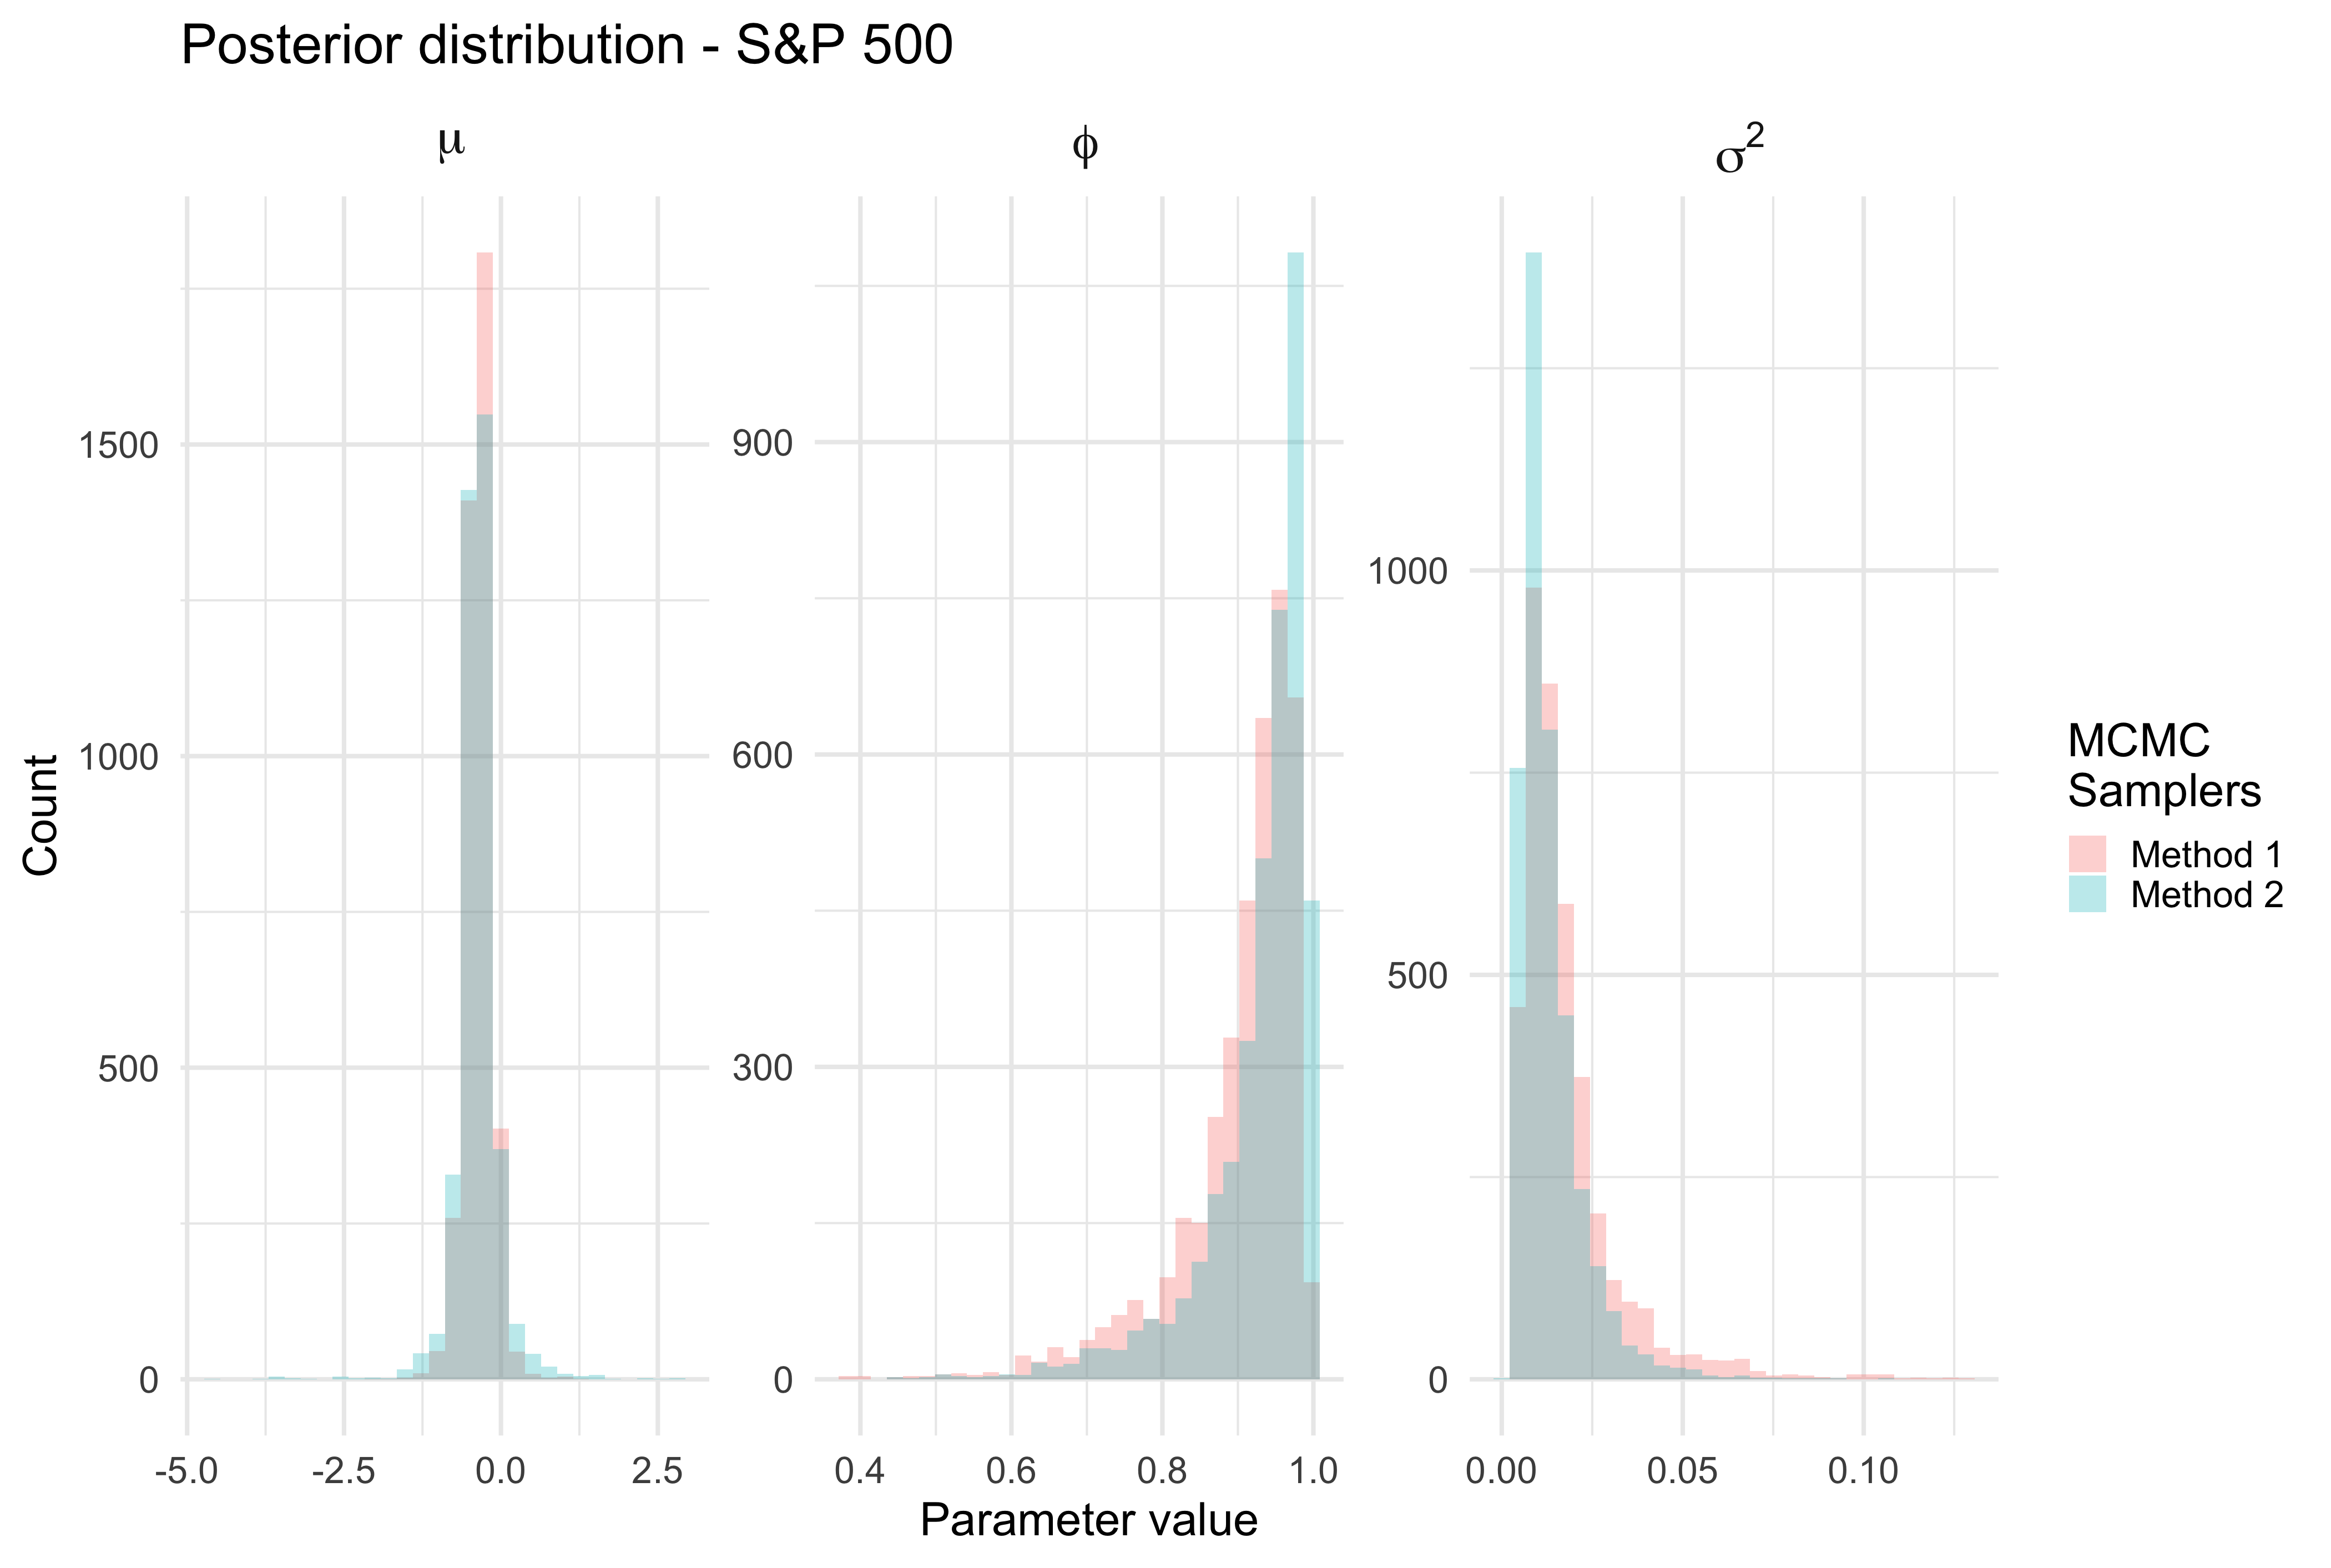
\includegraphics[scale=0.1]{motivating_example/real_data_ex.png}
        \caption{Posterior samples from the Hamiltonian Monte Carlo (HMC) and Kim Sherphard and Chib (KSC) MCMC samplers using S\&P 500 data. While the shape of the distributions are similar, the modes of HMC is much higher and the tails of KSC are fatter for $\phi$ and $\sigma^2$. Convergence diagnostics do not tell us which estimate is more correct since we don't observe the true model or true data generating process.}
        \label{fig:realdataex}
    \end{figure}

    \begin{table}[H]
        \centering
        \begin{tabular}{|c|c|c|c|c|c|c|c|} \hline 
        Parameter&  MCMC&Min& q25&  Median& Mean & q75&Max\\ \hline 
        $\mu$&  KSC&-2.03 & -0.472 & -0.354 & -0.355 & -0.231 & 1.31 \\
     $\mu$&  HMC&-4.55 & -0.508 & -0.373 & -0.370 & -0.229 &2.86  \\\hline 
     $\phi$&  KSC&0.384 & 0.875 & 0.928 & 0.902 & 0.958 & 0.997 \\
     $\phi$&  HMC&0.438 & 0.910 & 0.953 & 0.929 & 0.977 &1.00  \\ \hline 
     $\sigma^2$&  KSC&0.00237 & 0.00891 & 0.0138 & 0.0178 & 0.0210 & 0.130 \\ 
     $\sigma^2$&  HMC&0.00209 & 0.00731 & 0.0105 & 0.0131 & 0.0159 &0.107 \\ \hline
        \end{tabular}
        \caption{Summary statistics for HMC and KSC algorithms. KSC's 25th quantile $\phi$ is smaller than HMC which is consistent with the fatter left tail. Similarly, the KSC's 75th qunatile for $\sigma^2$ is larger consistent with a larger right tail spread. Both sets of estimate are reasonable but it is unclear from estimates on real data which estimate is closer the the truth.}
        \label{tab:realdata}
    \end{table}
    
\subsection{Diagnostic limitations on a single simulation}
    Diagnosing computational problems on real data is difficult due to confounding factors. A strategy around this is to evaluate a model and algorithm on simulated data. One approach is to simulate data from a generative model using known parameters. Then fit the same model on the simulated data and see if the true parameters can be recovered. This gives us the benefit of defining the true parameters of the data generating process to be estimated. If the model and algorithm cannot adequately capture the true parameter, then we cannot be confident that it will provide reliable estimates on real data.

    Furthermore, as discussed in \citet{gelman2020bayesian}, fitting models on simulated data is the only way we can check inference on latent variables. This is critical in stochastic volatility since the underlying framework is a state space model with latent log volatility parameters. Latent variables are unobserved in real data and are only estimated in the context of the model. Simulation gives control over the data generating process which reveals what the model can infer about the latent variables. 

    Simulations enable us to check whether our models and algorithms can estimate the true data generating process. However, there are limitations to what can be learned from a single simulation. There is always a small probability that the true parameter is in the tails of any estimated posterior distribution. Or put differently, there is a 1\% chance the true parameter or any random draw exists outside a 99\% credible interval. \cite{talts2018validating} make the point that a single simulation does not provide sufficient information about the inference made by an algorithm. As discussed in their paper, a single simulation may conclude ``that an incorrectly coded analysis worked as desired, while a correctly coded analysis failed''. 

    Figure 2 show the posterior distributions of a single simulation where data is generated and posteriors are sampled from the stochastic volatility model with known parameters.

    \begin{figure}[h]
        \centering
        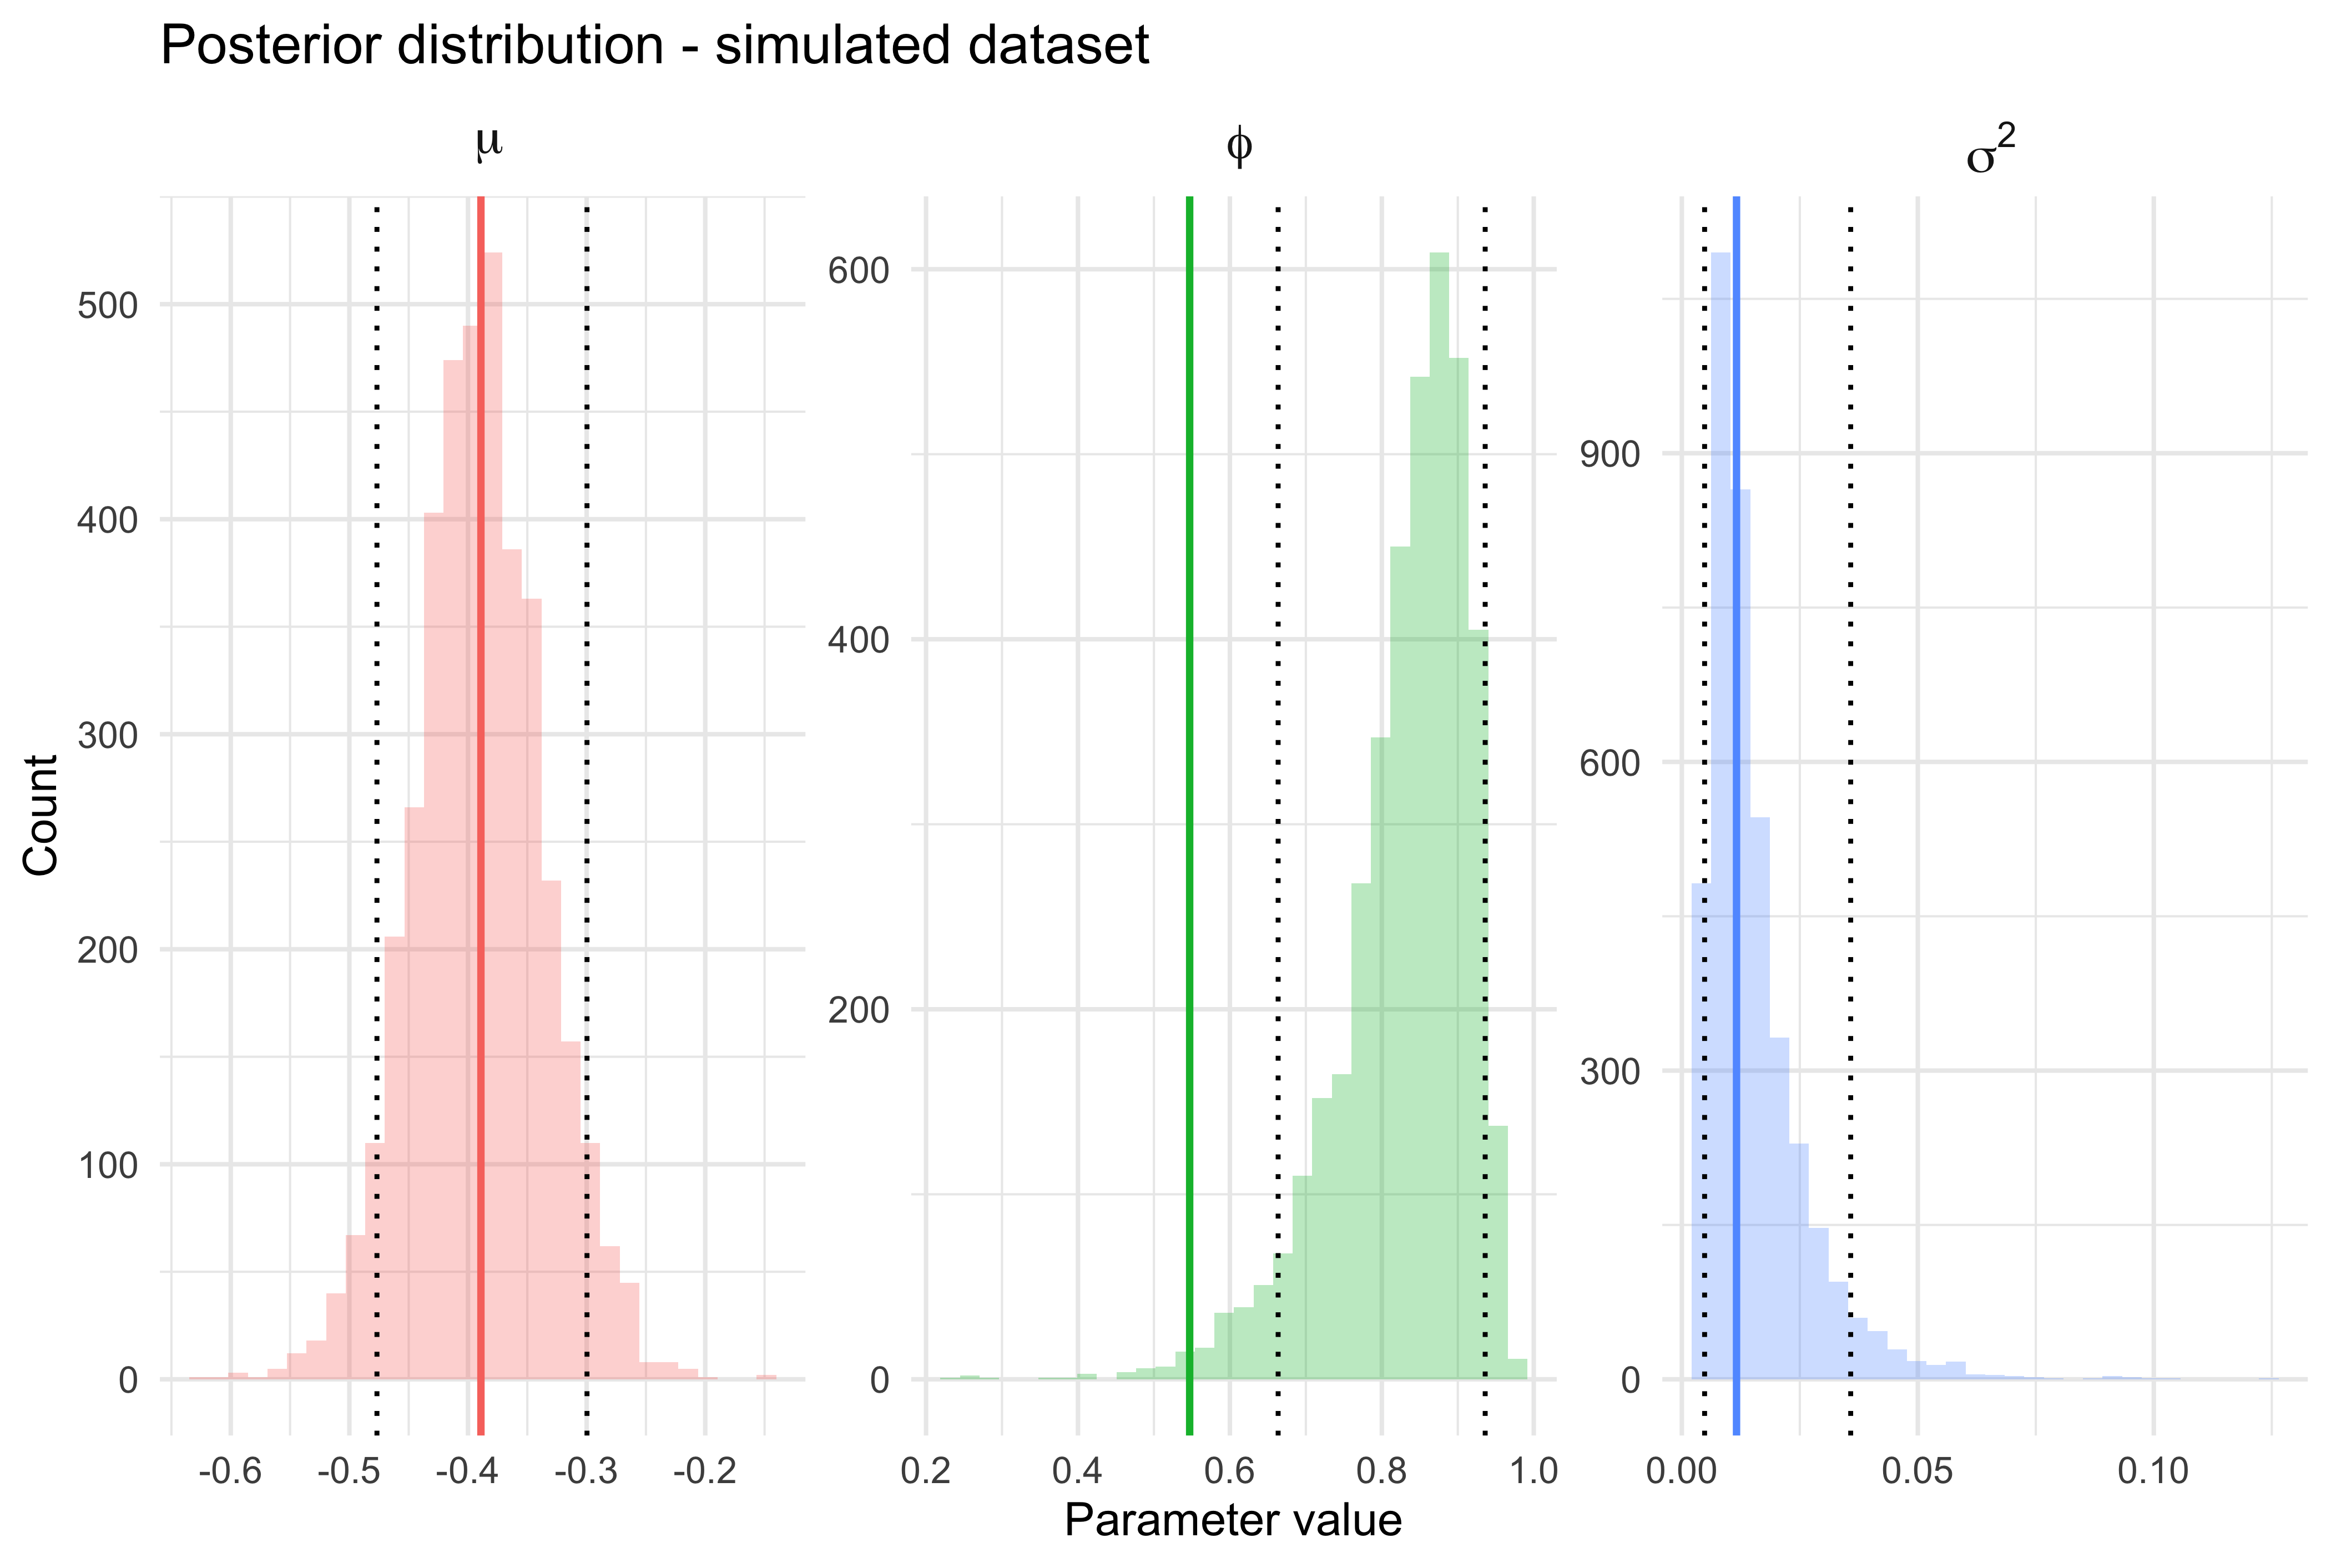
\includegraphics[scale=0.1]{motivating_example/single_sim.png}
        \caption{Posterior samples from known data genearting process. Vertical solid line represents true parameter and dotted lines are 95\% credible intervals around the mean. The parameter $\phi$ falls outside the credible interval whereas $\mu$ and $\sigma^2$ stay inside. In any one simulation conditional on the correct model, there is a 5\% probability that the true parameter falls outside this interval by chance.}
    \end{figure}

    The 95\% credible intervals for $\mu$ and $\sigma^2$ cover the true parameter. The true parameter for $\phi$ however, is in the tails and outside the interval. Such an analysis may incorrectly conclude that the model fails to adequatly estimate the $\phi$ parameter. However, it may be the case that the posterior distribution is correctly calculated using this algorithm and the results may be due to the features of this specific simulated dataset.

\subsection{Research Goal}
    The objective of this research is to design a simulation study to evaluate the calibration of algorithms used to estimate stochastic volatility models. As discussed, there are limitations to evaluating MCMC algorithms based on fits to real data and single simulations. To check the calibration of an algorithm, simulations over multiple true parameters are required. This methodology is discussed in the next section. 

    Additionally, both the HMC and KSC algorithms will be assessed using the proposed simulation design as well as the performance of the samplers under different parameterisations of the stochastic volatility model. Results from the study will also be used to compare both sampling strategies to determine which MCMC approach is most suitable for estimating this model. 

\section{Methodology}

    \subsection{Simulation Design}
        Simulation Based Calibration (SBC) checks the calibration of posterior estimates generated by MCMC algorithms. SBC is conducted by comparing the distribution of rank statistics to the discrete uniform distribution which arises when an algorithm is correctly calibrated. The procedure starts by taking draws from the prior distribution and creating datasets implied by each draw. Rank statistics are then calculated on the posterior samples conditional on the simulated data. 

        To illustrate this procedure, let $\theta$ be an arbitrary parameter from a model and $y$ represent a dataset. Start with a single draw from the prior distribution:
        
        $$
        \begin{aligned}
        \theta^{sim} \sim \pi(\theta)
        \end{aligned}
        $$

        Generate a dataset given by the prior draw.

        $$
        \begin{aligned}
        y^{sim} \sim \pi (y|\theta^{sim})
        \end{aligned}
        $$

        Then take draws from the posterior distribution generated by a MCMC algorithm (HMC or KSC) conditional on this dataset.

        $$
        \begin{aligned}
        \{\theta_1,\dots , \theta_{L}\} \sim \pi (\theta | y^{sim})
        \end{aligned}
        $$

        A key result is that the posterior sample $\{\theta_1,\dots , \theta_{L}\}$ will share the same distribution as the prior samples $\theta^{sim}$. This is implied by the following expression:

        $$
        \begin{aligned}
        \pi(\theta) &= \int \pi(\theta|y^{sim}) \pi(y^{sim}|\theta^{sim}) \pi(\theta^{sim})dy^{sim} d\theta^{sim} \\
        &= \int \pi(\theta|y^{sim}) \pi(y^{sim},\theta^{sim}) dy^{sim} d\theta^{sim}
        \end{aligned}
        $$

        That is, the posterior averaged over the joint distribution follows the same distribution as the prior. The procedure of generating posterior samples implicitly performs this integral since the expression on the right of the integral is proportional to the prior density. Therefore, any deviation of the posterior distribution from the prior distribution means that the sampling methodology is not producing the correct posteriors.

        \citet{talts2018validating} prove that the rank statistics for a given parameter follows a discrete uniform distribution if the posterior samples follow the same distribution as the prior. The rank statistic is defined as:

        $$
        \begin{aligned}
        r = rank(\{\theta_1,\dots , \theta_{L}\}, \theta^{sim}) = \sum_{l=1}^{L}1[\theta_{l} < \theta^{sim}]
        \end{aligned}
        $$

        This completes one iteration of SBC. To complete the algorithm, multiple iterations are run and the rank statistics are calculated for each parameter. The resulting rank statistics are compared to the discrete uniform distribution to determine if the algorithm is calibrated and returning the correct posteriors.

        Posterior credible intervals are said to have sufficient coverage if Bayesian computation is well calibrated and the rank statistics follow a discrete uniform distribution. That said, there are two ways to interpret calibration. 

        \begin{enumerate}
            \item For any percentage interval selected over the posterior samples (for example 90\%) then there is a 90\% chance that $\theta^{sim}$ falls within this interval.
            
            \item Bayesian analysis is well calibrated if a 90\% credible interval contains the true parameter in 90\% of the SBC iterations. 
        \end{enumerate}
        
        % That is, one way to describe calibration is: for any percentage interval selected over the posterior samples (for example 90\%) then there is a 90\% chance that $\theta^{sim}$ falls within this interval. Another way of saying this is a Bayesian analysis is well calibrated if a 90\% credible interval contains the true parameter in 90\% of the SBC iterations. 

    \subsection{Evaluation Metrics}
        The key metrics to compare the performance of these methods are rank statistics and chi-squared test statistics to measure calibration, and the effective sample size (ESS) to measure effciency.

        \subsubsection{Rank statistics}
            Rank statistics are used to evaluate the calibration of the MCMC algorithm. If a posterior is well calibrated then it is expected that the distribution of rank statistics is uniform.

            The shape of the rank statistic distribution gives insight into how a MCMC may be miscalibrated. Specifically, it gives information about the type of bias in the posterior estimates for a given parameter. Figures \ref{fig:underestimation} and \ref{fig:underdispersed} are recreated from \citet{talts2018validating} for convenience which display examples of posterior estimates that give biased rank statistics.

            Figure \ref{fig:underestimation} shows a distribution of rank statistics with a large right peak. This is consistent with posterior samples underestimating the true parameter, where the estimated posterior distrubtion is biased to the left of the prior. The sum of indicator random variables is large since the majority of posterior draws are smaller than the true value. This results in a large rank statistic and a bias on the right side of the histogram. The coverse is true if the peak of the histogram is on the left hand side (i.e the posterior is biased towards the right hand side of the prior). 

            Figure \ref{fig:underdispersed} has large peaks on both ends of the histogram. The sampler is disproportionately over and under estimating the true parameter. \citet{talts2018validating} describe this bias as underdispersion of the posterior relative to the prior distribuion. The estimated posterior is too narrow relative to the spread of the prior resulting in bias on both ends of the rank statistic distribution. 

            % \begin{figure}[H]
            %     \centering
            %     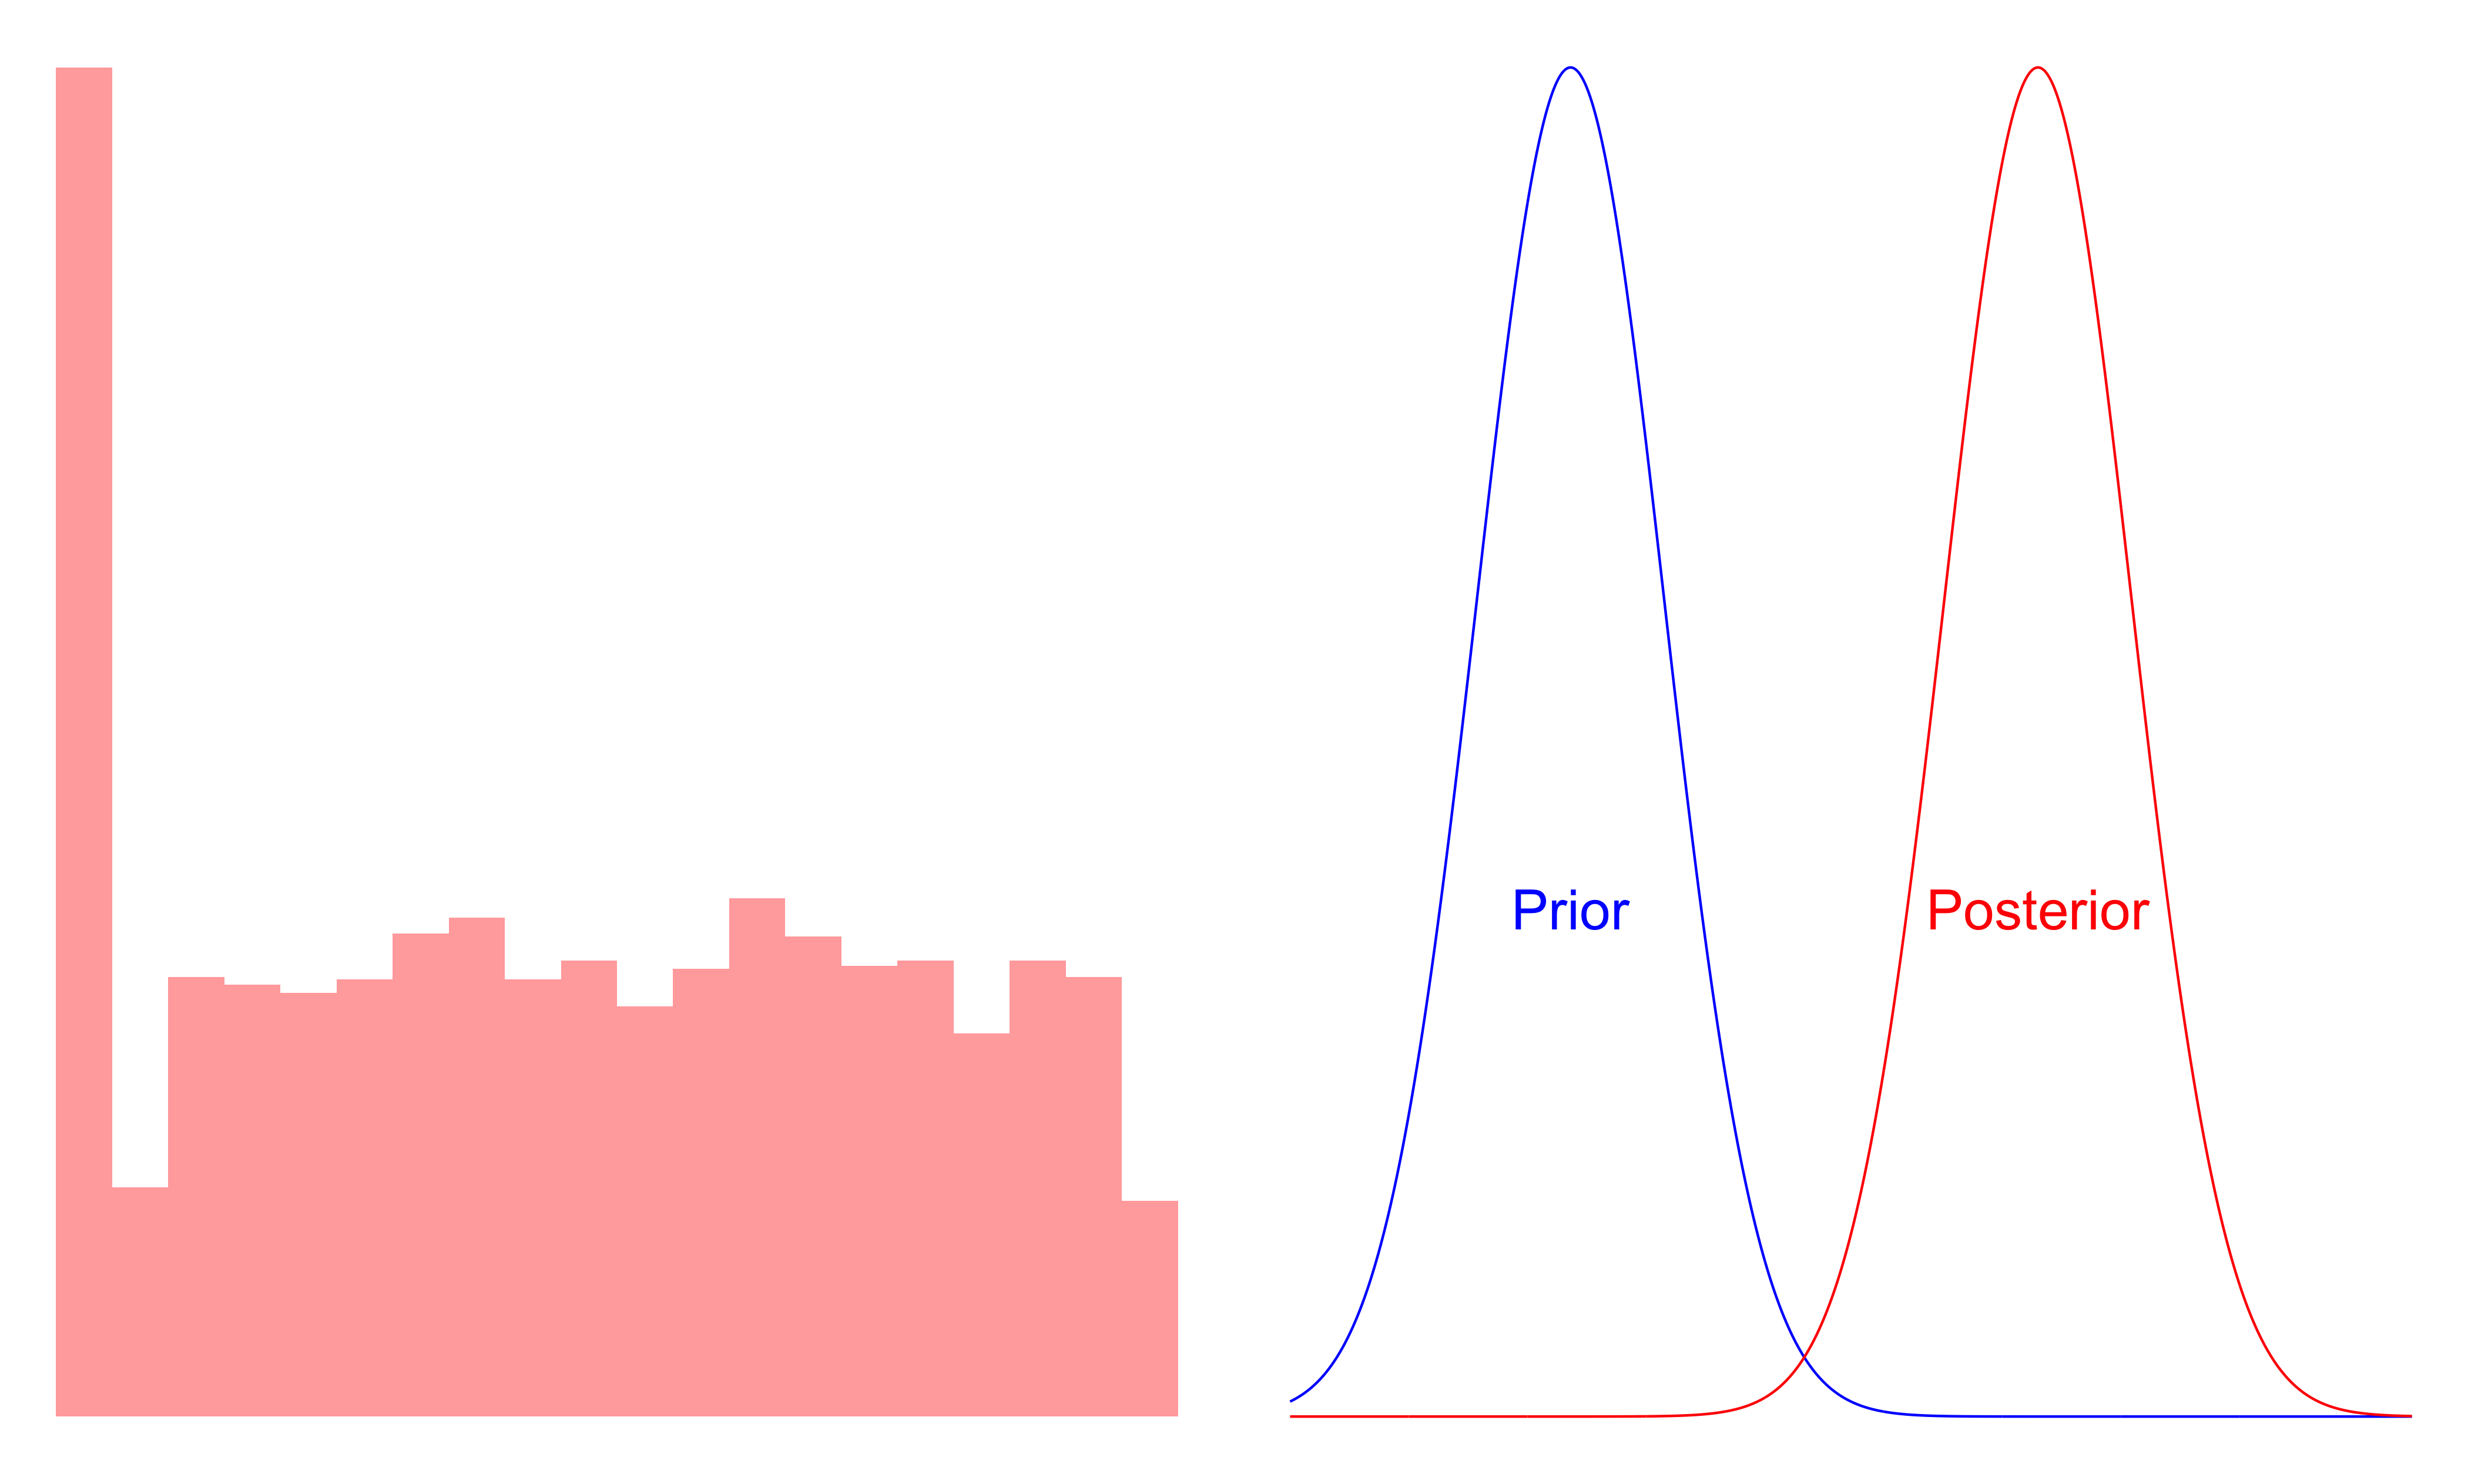
\includegraphics[scale=0.07]{methodology/lhs.png}
            %     \caption{Left: Non uniform rank statistics with peak on the left side. Right: Posterior distribution vertical line representing true parameter. Bias in rank statistics distribution comes from disproportionate number of SBC iterations overestimating the true parameter.}
            %     \label{fig:overestimate}
            % \end{figure}
        
            \begin{figure}[H]
                \centering
                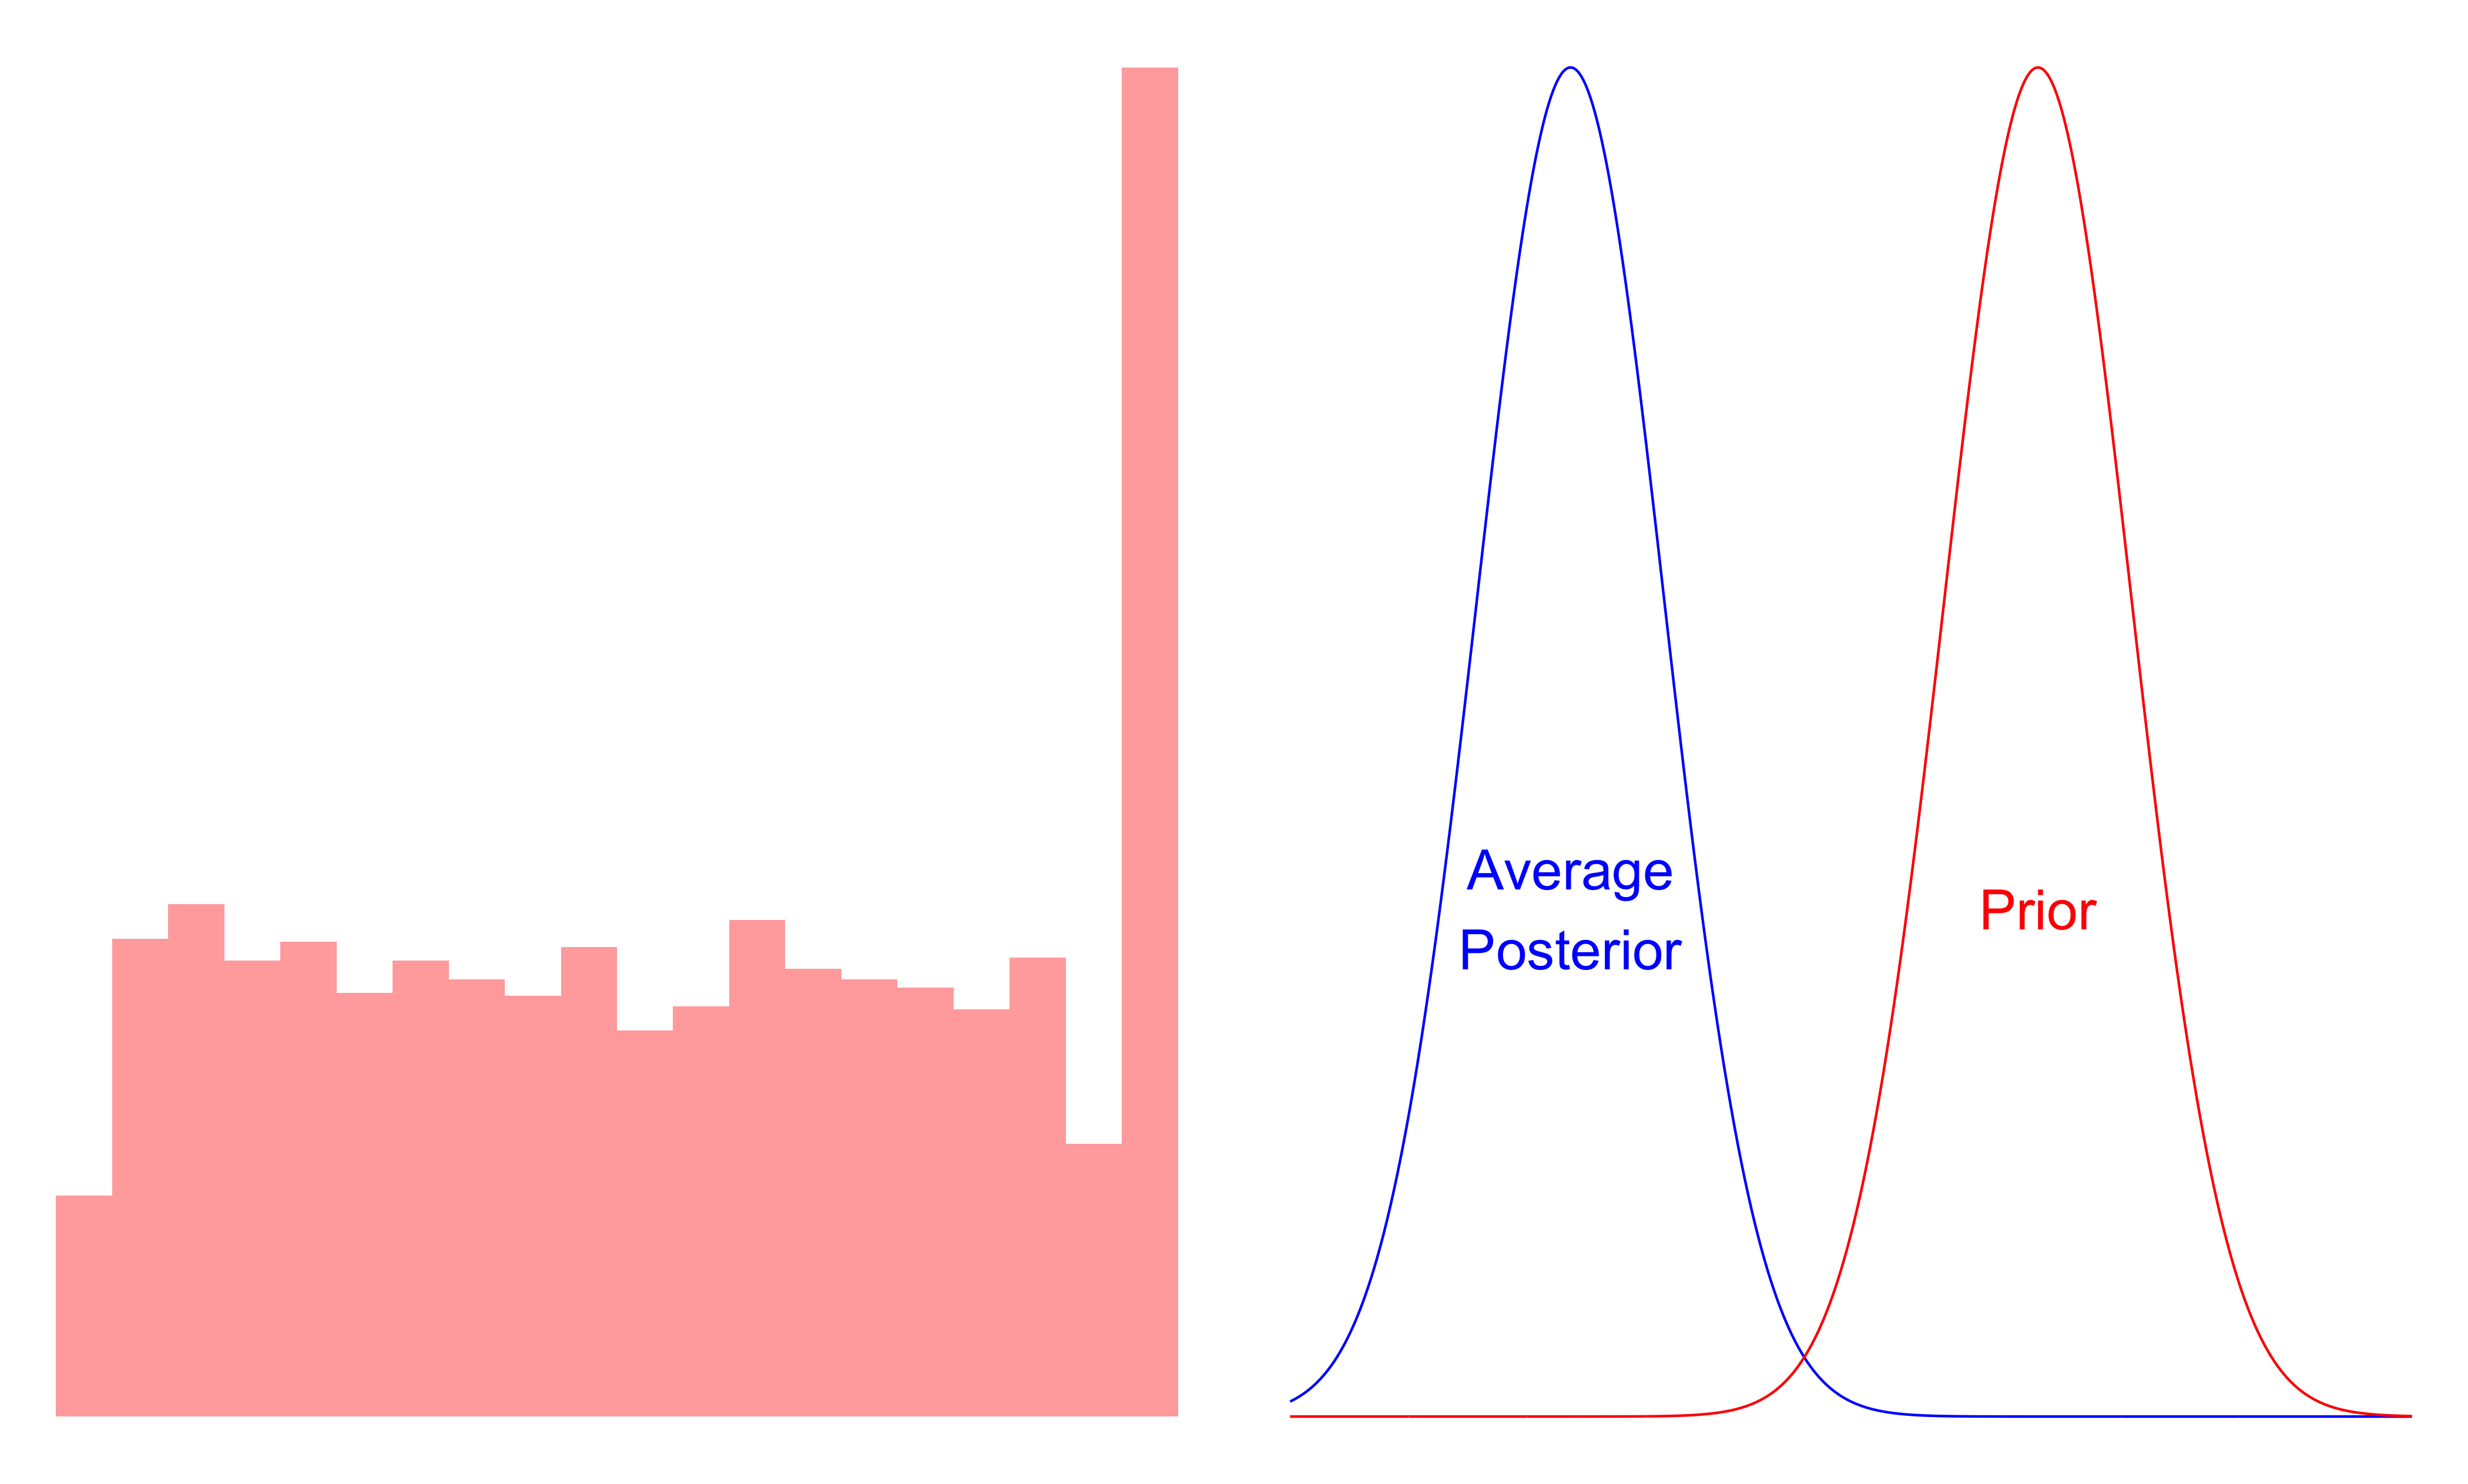
\includegraphics[scale=0.07]{methodology/rhs.png}
                \caption{Left: Non uniform rank statistics with peak on the right side. Right: Posterior distribution is biased to the left side of the prior distribution. Bias in rank statistics distribution comes from disproportionate number of SBC iterations underestimating the true parameter. Note that the two plots are independently produced for illustration only.}
                \label{fig:underestimation}
            \end{figure}        

            \begin{figure}[H]
                \centering
                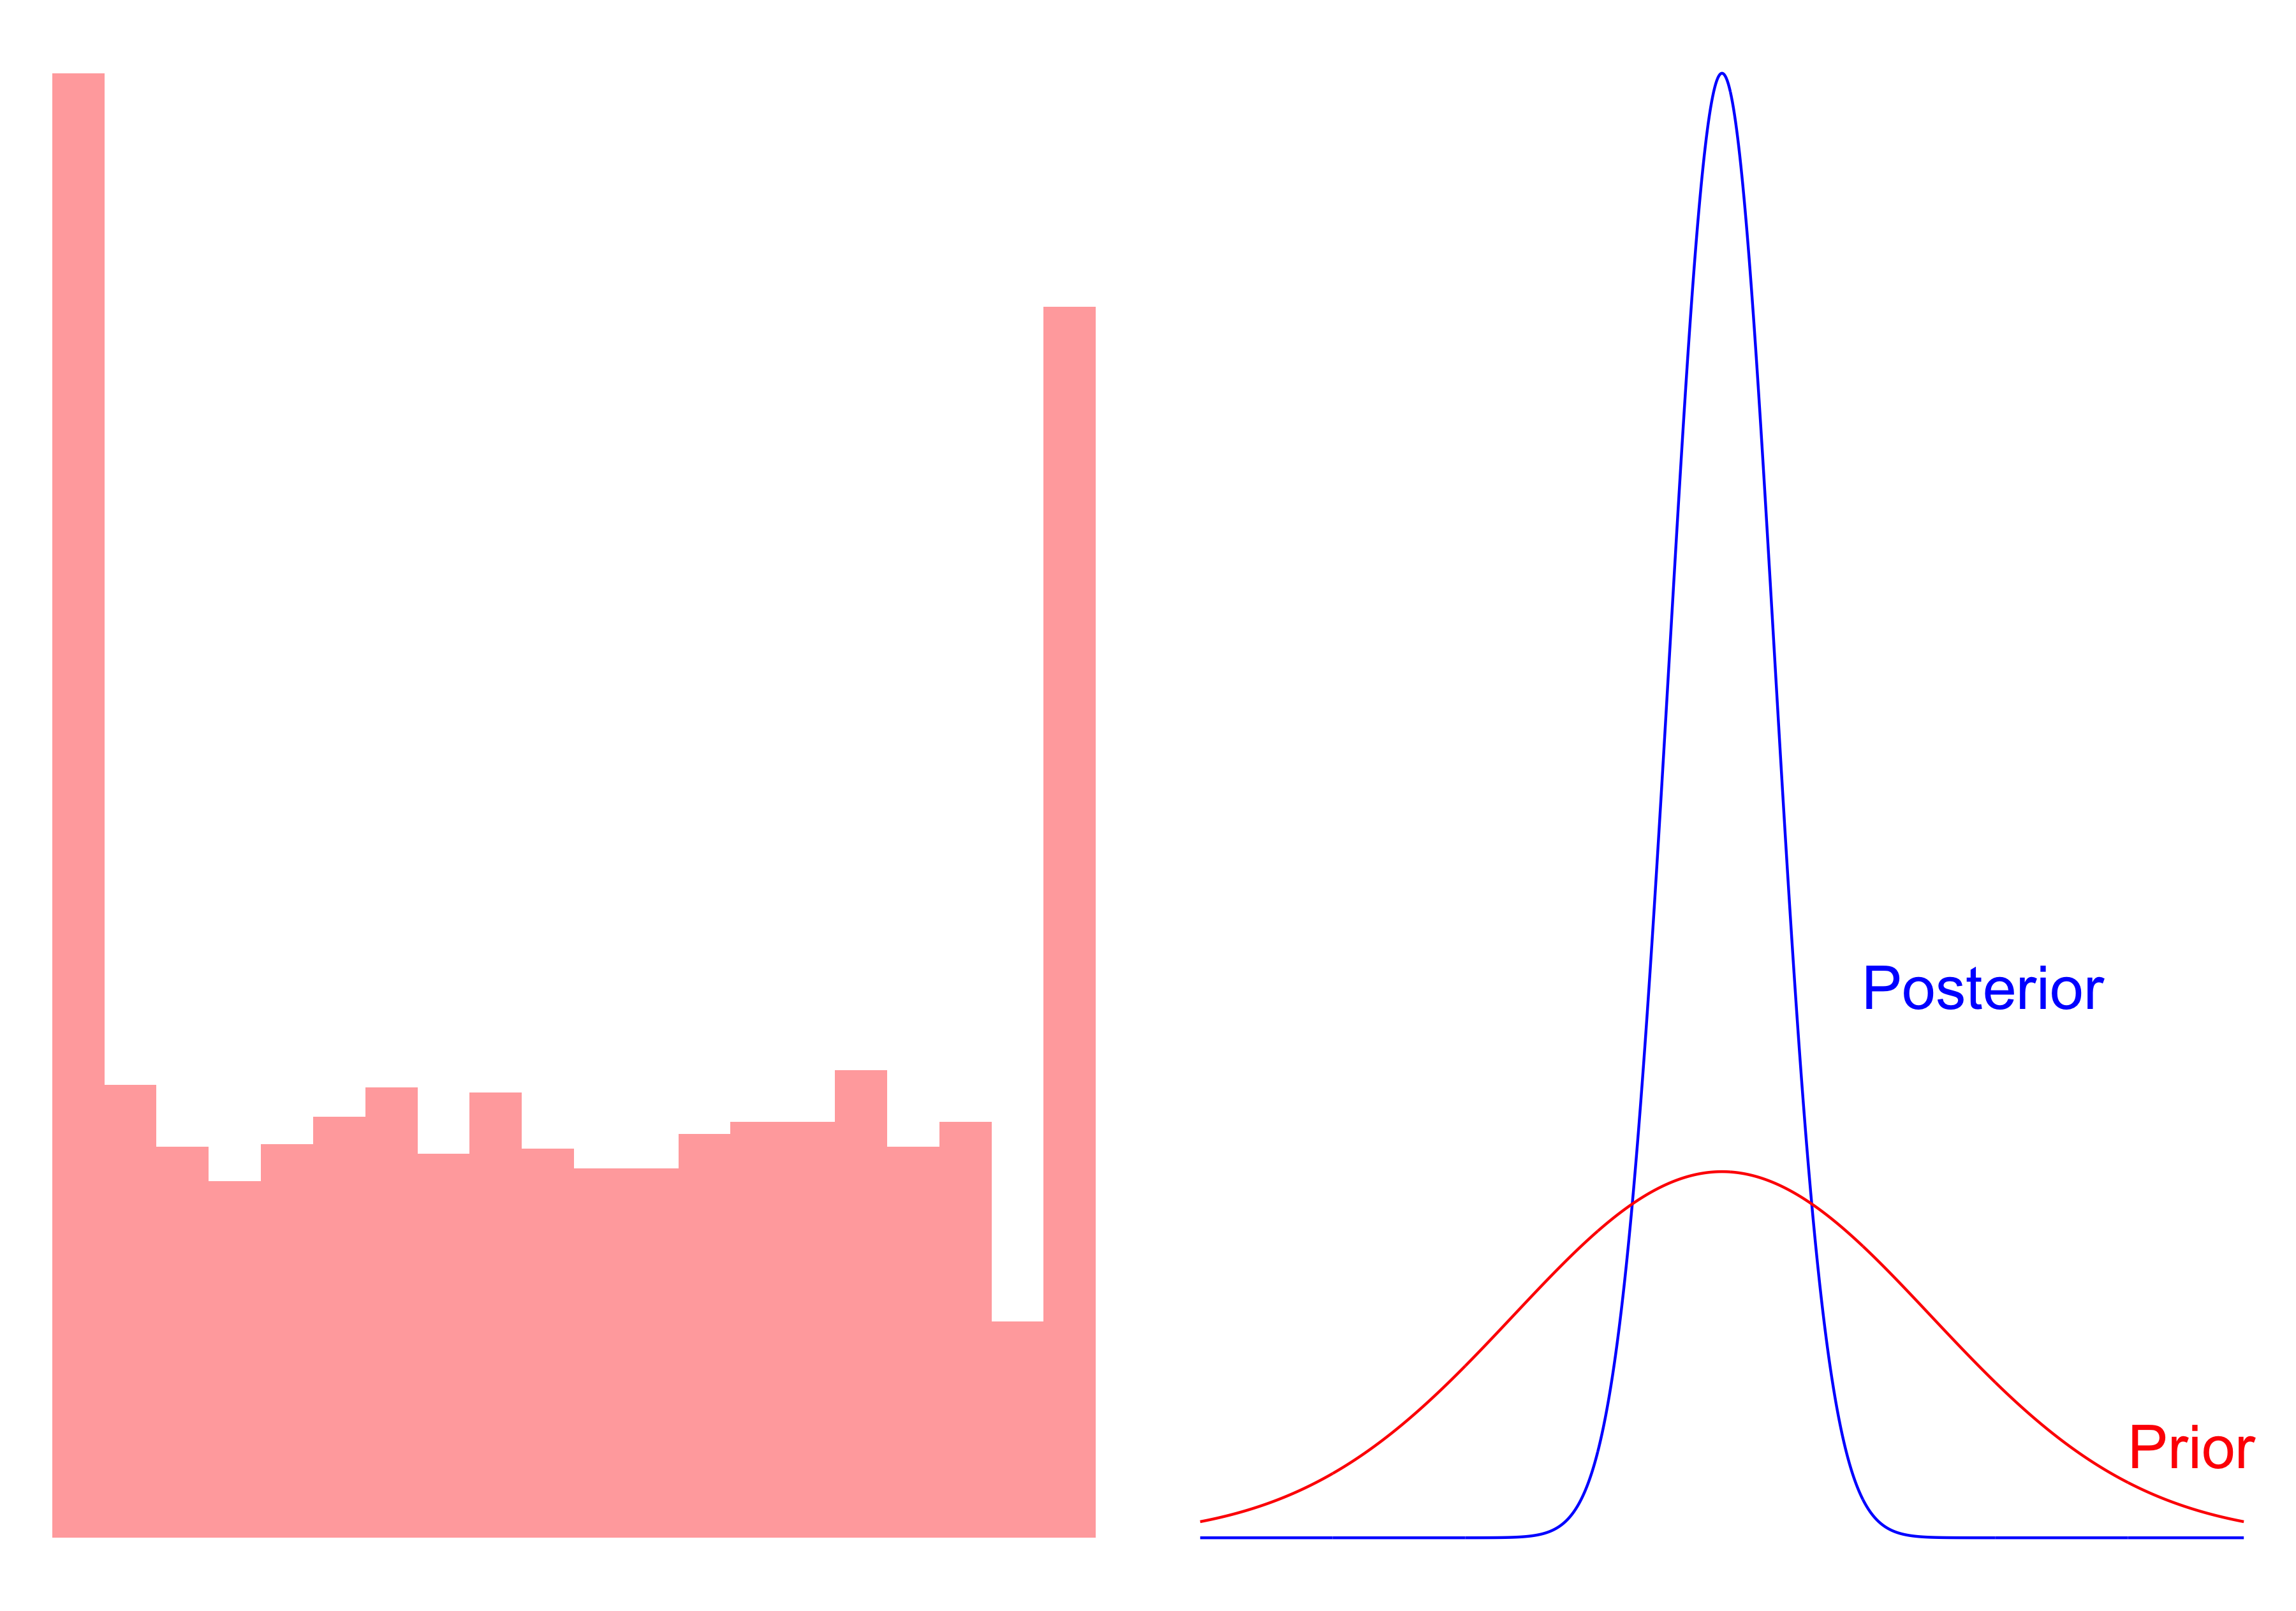
\includegraphics[scale=0.07]{methodology/underdispersed.png}
                \caption{Left: Non uniform rank statistics with peaks on both ends. Right: Overlayed posterior and prior distributions for the same arbitrary parameter. Bias in ranks comes from underdispersed posterior distribution relative to prior.}
                \label{fig:underdispersed}
            \end{figure}

            \subsubsection{Chi squared statistics}
            A drawback from visualising the rank statistic distributions is there are more parameters and latent states to estimate than data points in this model. An alternative to visually checking for uniformity of all the parameters is to calculate the chi squared statistics for the counts in each histogram bin. Let $b_j$ be the number of counts and $e_j$ the expected count in bin $j$ (where the expected count is a function of the number of bins and data points under a discrete uniform distribution). Then the chi squared statistic is given by:
            
            $$
            \begin{aligned}
            \chi^2 = \sum_{j=1}^J \frac{(b_{j} - e_{j})^2}{e_j}
            \end{aligned}
            $$
            
            A perfectly discrete uniform distribution will return a chi squared statistic of zero. That is, the number of rank statistics in each bin is equal to the expected count under a discrete uniform distribution. The distribution of chi squared statistics is visualised to compare results across multiple simulations. This will give a high level summary of calibration and overall performance of the algorithms.

            \subsubsection{Effective sample size}
            ESS measures the efficiency of the MCMC sampler. It calculates the number of effectively independent draws generated by a MCMC to estimate a target parameter. A poor ESS can arise from high autocorrelation in the Markov chain which leads to highly dependent samples. An efficient MCMC algorithm takes less resources (for example, time and number of draws) to get a representative sample of the target distribution. If a MCMC algorithm possesses higher ESS for the majority of its parameters (relative to another strategy), then there is evidence that this method is a more efficient sampler.
            
            The ESS is defined as $n_{eff}$ and is a function of the number of chains $M$, the number of samples per chain $N$ and the autocorrelation at lag t $\rho_t$. $T$ is a trunction lag chosen such that the sum of any two consecutive autocorrelation lags is negative. This truncation (or some kind of downweighting) is required because a large number of lags leads to noisier autocorrelation estimates. More details about this ESS formula and the calculation of the autocorrelation can be found in \citep{vehtari2021rank} and \citet{geyer1992practical}.

            $$
            \begin{aligned}
                n_{eff} = \frac{NM}{1+2 \sum_{t=1}^T \hat{\rho}_t}
            \end{aligned}
            $$

\section{MCMC Strategies}

    \subsection{Sampling method 1}
        KSC sample the posteriors of the stochastic volatility model using a mix of conjugate posterior distributions, Metropolis Hastings and the Kalman Filter and smoother\footnote{In this research the exact software to apply the simulation smoother is unavailable. So a more recent simulation smoother is used which is written by the same author of the original software.} \citep{dejong1995}.

        The standard Kalman Filter and simulation smoother is used to compute the posterior distribution over the latent states. This requires the state and measurement equations to be linear and conditionally Gaussian. Since the relationship between $y_t$ and $h_t$ in the measurement equation is not linear, a transformation is applied by squaring and taking the log of $y_t$.

        $$
        \begin{aligned}
        y_t^{*} &= log(y_t^2) \\ 
        &= log((\epsilon_t exp(h_t/2))^2) \\
        &=  log(exp(h_t)) + log(\epsilon_t^2) \\
        &= h_t + log(\epsilon_t^2)  \\
        &= h_t + z_t \\
        \end{aligned}
        $$

        Where $z_t = log(\epsilon_t^2)$ follows a log chi-squared distribution with mean -1.2704 and variance 4.93. The relationship between $y_t$ and $h_t$ is now linear; however, the error is not Gaussian. Since it is not simple to sample from this parameterisation of the model, KSC use a mixture of Gaussians to approximate the first 4 moments of the log chi squared distribution. This is defined by:

        $$
        \begin{aligned}
        f(z_t) = \sum_{i=1}^{K} q_if_N(z_i|m_i-1.2704, \nu_i^2)
        \end{aligned}
        $$

        Where K is the mixture of normal densities $f_N$, component probabilities $q_i$, mean $m_i-1.2704$ and variance $\nu_i^2$. These parameters were selected using moment matching where they found 7 normal densities with varying mean and variance parameters best approximated the log chi squared moments. These parameters and weights can be found in Appendix A.

        The model can be sampled via the Kalman Filter and simulation smoother since the model is now linear and conditionally gaussian. The static parameters $\mu$ and $\sigma^2$ are sampled directly from their conjugate posterior distributions whereas $\phi$ is sampled via a Metropolis Hastings accept/reject procedure. The details can be around in Appendix B. 

        \subsubsection*{Implementation}
        The code used to replicate the KSC algorithm was written by \citet{chad2018} and ammended for the purposes of this research. Additional code was developed to produce rank statistics, quantities of interest as well as to integrate the MCMC into the SBC framework. 
        
        The steps in the MCMC process is desribed in Algorithm \ref{alg:ksc}. The initial values are set to the values outlined in \citet{kim1998stochastic}, except for the mixing indicator which is unspecified. This is arbitrarily set at the 4th Gaussian density found in Appendix A.

        For sampling the mixture model the Gaussian mixture density is rewritten with respect to a indicator variable $s_t$

        $$
        \begin{aligned}
        &z_t | s_t = i \sim N(m_i - 1.2704, \nu^2) \\
        &Pr(s_t = i) = q_i
        \end{aligned}
        $$
        
        $s_t$ is then sambled from probability mass function: 
        
        $$
        \begin{aligned}
        Pr(s_t = i | y_t^{\ast}, h_t) \propto q_i f_N(y_t^{\ast} | h_t + m_t - 1.2704, \nu^2)
        \end{aligned}
        $$

        \begin{algorithm}[H]
            \caption{KSC MCMC Algorithm}\label{alg:ksc}
            \begin{algorithmic}
            \Require $s_0 = 4$, $\mu_0 = 0$, $\phi_0 = 0.95$, $\sigma^{2}_{\eta,0} = 0.02$
            \For{\texttt{i in} $1:n_{draws}$}
                    \State \text{Sample states (Kalman Filter and Smoother): } $\boldsymbol{h}_i \sim h|y^{\ast}, s_{i-1}, \phi_{i-1}, \sigma^{2}_{\eta,i-1}, \mu^{i-1}$ 
                    \State \text{Sample mixture density: } $s_i \sim s|y^{\ast}, \boldsymbol{h}_{i-1}$
                    \State \text{Sample conjugate density $\mu$: } $\mu_i \sim \mu|y_{\ast}, s_{i-1}, \phi_{i-1}, \sigma^{2}_{\eta, i-1}, \boldsymbol{h}_{i-1}$
                    \State \text{Sample conjugate density $\sigma^2_{\eta}$: } $\mu_i \sim \mu|y^{\ast}, s_{i-1}, \phi_{i-1}, \mu_{i-1}, \boldsymbol{h}_{i-1}$
                    \State \text{Metrpolis Hastings step $\phi$: } $\phi_i \sim \phi|y^{\ast}, s_{i-1}, \mu_{i-1}, \sigma^{2}_{\eta, i-1}, \boldsymbol{h}_{i-1}$
                  \EndFor
            \end{algorithmic}
            \end{algorithm}

    \subsection{Sampling method 2}
        Hamiltonian Monte Carlo (HMC) is a MCMC algorithm which has become widely available for efficiently sampling sophisticated models. Hamiltonian Monte Carlo, originally called Hybrid Monte Carlo, was developed in the physics literature \citep{duane1987hybrid} before being applied in the statistics literature by Radford Neal through his works in Bayesian Neural Networks \citep{neal1995bayesian} and statistical computing \citep{neal2011mcmc}. The algorithm has since become widely available through open source development projects such as Stan \citep{stan} and PyMC \citep{pymc2023}.

        The key innovation of HMC is using the gradients of the target posterior distribution to generate an efficient path for the sampler to explore. HMC is able to reach more distant points with higher acceptance probabilites since proposals are made with information about the target distribution. Random walk samplers are become inefficient in higher dimensions since it is more difficult to randomly select a point with a high acceptance probability. The increasing complexity of high dimensions make it harder for a random walk sampler to explore regions over long distances, resulting in the sampler to become stuck and requiring a lot of iterations to converge onto the target distribution. 

        A thorough conceptual and theoretical explanation of HMC can be found in \citet{gelman2013bayesian} and \citet{betancourt2017conceptual} with further details found in the aforementioned literature. HMC builds upon the Metropolis Hastings algorithm through the introduction of Hamiltonian equations, auxiliary momentum variables $\phi$, and the gradients of the target log posterior distribtuion. The vector of model parameters $\theta$ is jointly sampled with a vector of momentum variables $\phi$. The momentum variables are also called auxiliary variables since they are required as part of the Hamiltonian equations to generate an efficient proposal but are not a quantity of interest for inference.

        The sampled momentum variable sets out the proposal path for $\theta$ governed by the Hamiltonian dynamics (represented by a set of differential equations). These differential equations are solved using a discrete approximation algorithm, such as a leapfrog integrator, and is a function of the log posterior gradients for a given point $\theta$. The leapfrog integrator has a set of tuning parameters which determines the size and number of steps to be taken along the Hamiltonian path with the final step being the proposal value $(\theta^{\ast}, \phi^{\ast})$. Finally, the Metropolis Hastings accept/reject step is applied using the parameters at the beginning of the leapfrog process $(\theta^{t-1}, \phi^{t-1})$ and the proposal values $(\theta^{\ast}, \phi^{\ast})$. A formal description of the HMC algorithm is provided in Appendix C.

        \subsubsection{Implementation}
        The Stan programming language's implementation of Hamiltonian Monte Carlo will be used for this study. Stan's default algorithm, the No-U-Turn Sampler \citep{hoffman2014no}, allows for direct sampling of the specified stochastic volatility model. Hamiltonian Monte Carlo allows for sampling of the generative model and can flexibly handle complicated likelihood functions. This approach will also use the same priors as specified in the KSC's Gaussian mixture approximation so that HMC is sampling from the same model (although other priors could be chosen). 

    \subsection{MCMC methods comparison}
        The KSC sampling method and HMC are both MCMC strategies to genereate samples from the target joint posterior distribution of the stochastic volatility model. However, the two sampling approaches are conceptually different in their design and implementation, despite sharing the same objective.
        
        The KSC sampling method is a bespoke algorithm designed specifically for the sampling of the stochastic volatility model. It is a strategy built around how to sample the parameters from the state space model in this specific context. The implementation of this MCMC requires careful attention to the sampling of each parameter using different tools and requires these components to be programmed manually, such as the Metropolis Hastings step and conjugate posterior distributions. 
    
        HMC on the other hand is a more general approach to applying MCMC. The implementation of HMC is through the Stan programming language which allows for the specfication other generative or Bayesian models, not just stochastic volatility. The implementation details of HMC is abstracted away from the user, who only needs to focus on specifying the model using the Stan syntax. Any hyperparameter tuning and initialisation is automated away. Furthermore, Stan and HMC allows for the specification of different priors, whereas KSC's bespoke algorithm is dependent on the use of conjugate priors. 

        The conceptual difference in both methods result in different tradeoffs. The abstraction of the MCMC implementation using the Stan programming language means users can focus more on the modelling and the applied research question. The algorithm is maintained by other developers and different models can be compared with each other without worrying about differences in MCMC implementations. However, the abstraction away from the details means there is less flexibility in MCMC design in the scenario where the current instance of Stan or HMC is insufficient for a specific model.
        
    \subsection{Model Parameterisation}

        The parameterisation of a model can affect the performance of a MCMC algorithm when sampling from models with complex posterior geometries. An example of this is Neal's funnel \citep{neal2003slice} where the Hamiltonian Monte Carlo sampler encounters performance issues in hierarchical models and produces biased samples. Efficiency improvements of MCMC algorithms for state space models under different parameterisations are also explored in \citet{strickland2008parameterisation}.

        The stochastic volatility model as described in section 2.1 is follows a centered parameterisation. This describes the central location of the latent state distribution which is centered on the mean of log volatility $\mu$. A model can be reparameterised in a way that improves MCMC performance. Reparameterisation applies a transformation to the model which may change the interpretation of the parameters or the way they are sampled but remains mathematically equivalent to the original model. The reparametiersations available for a model is dependent on the MCMC approach. Some reparamterisations are available only to specific sampling strategies and may improve or impair a MCMC performance. 

        SBC is applied to reparameteirsied versions of the stochastic volatility model to see if there is any improvement in calibration and efficiency. 
        
        \subsubsection{Reparameterised stochastic volatility for Hamiltonian Monte Carlo}
        The reparameterisation for Hamiltonian Monte Carlo changes how the latent states are sampled. Specifically, the states are first sampled from a standard normal distribution and are transformed to be samples from the state equation. As noted above, the centered parametersation samples the states centered around $\mu$.  

        First sample from a standard normal distribuition and multiply by the variance of the log volatility. The state vector is sampled with mean centered on zero and variance equal to $\sigma_{\eta}^2$

        $$
        \begin{aligned}
        h_{std} \sim& \space normal(0,1) \\
        h =& h_{std} \times \sigma_{\eta} \\ 
        h \sim& normal(0, \sigma_{\eta}^2)
        \end{aligned}
        $$
        
        Then apply the appropriate rescaling to get samples from log volatility. 
        
        $$
        \begin{aligned}
        h_1 =& \space \frac{h_{std, 1}\times \sigma_{\eta}} {\sqrt{1 - \phi^2}} + \mu \\
        h_{t+1} =& \space h_{std, t+1}\times \sigma_{\eta} + \mu  + \phi(h_{t} - \mu),\space t\neq 1
        \end{aligned}
        $$
        
        This returns log volatility as desired.
        
        $$
        \begin{aligned}
        h_1 \sim& \space normal \left(\mu, \frac{\sigma_{\eta}^2}{1-\phi^2}\right) \\
        h_{t+1} \sim& \space normal(\mu +\phi(h_t - \mu) , \sigma_{\eta}^2), \space\space t\neq 1\\ 
        \end{aligned}
        $$

        \subsubsection{Non centered Gaussian Mixture model}
        The reparameterised model for the Gaussian approximation is expressed differently due to the Kalman Filter. Reparameterised HMC samples from the joint posterior directly with state vectors centered at zero and transformed to return the correct log volatility estimates. Applying the Kalman Filter requires the state equation to be a function of the state variable with the average log volatility parameter $\mu$ entering the measurement equation.

        The following parameterisation is described as non centered in location. This follows the methodology outlined in \citet{strickland2008parameterisation}.
        
        Starting with the log chi squared model:

        $$
        \begin{aligned}
        y^{\ast}_t =& h_t + z_t \\
        h_{t+1} =& \space \mu +\phi(h_t - \mu) + \sigma_{\eta} \eta_t
        \end{aligned}
        $$
        

        Let $g$ be the demeaned state variable. Rewrite the demeaned state equation $g_{t+1}$ to be non centered in location by subtracting average volatility $\mu$.

        $$
        \begin{aligned}
        g_t =& h_t - \mu \\
        g_{t+1} =& \phi g_t + \sigma_{\eta}\eta_{t}
        \end{aligned}
        $$

        Return average volatility into measurement equation and rewrite as a function of the non centered state equation:

        $$
        \begin{aligned}
        y^{\ast}_t =& g_t + \mu + z_t \\
        g_{t+1} =& \phi g_t + \sigma_{\eta}\eta_{t}
        \end{aligned}
        $$

        The mean of the log volatility is now inside the measurement equation and de-meaned from the state equation.
    
    \subsubsection{Prior Predictive check}
        % Different parameteristions express the same mathematical models in ways that make it easier or harder for a given algorithm to sample. 
        A prior predictive simulation of the second state parameter is performed for both a centered and reparameterised model using the approach described in Section 4.4.1. This is to demonstrate that different parameteristions express the same underlying mathematical model. This is similar the first two steps of SBC, except instead of generating a dataset, generate the state variable implied by the prior draw. Let $\boldsymbol{\theta}$ be a vector of static parameters. Simulate a draw from the joint prior:

        $$
        \begin{aligned}
        \boldsymbol{\theta}^{sim} \sim \pi(\boldsymbol{\theta})
        \end{aligned}
        $$

        Generate a the second state parameter conditional on prior simulation and first state variable.

        $$
        \begin{aligned}
        h_2^{sim} \sim \pi (h_2|h_1, \boldsymbol{\theta}^{sim})
        \end{aligned}
        $$

        Simulating 1000 samples of $h_2^{sim}$ from both centered and non-centered models gives samples from the same data generating process as shown in Figure \ref{fig:priorpred}. 


        \begin{figure}[h]
            \centering
            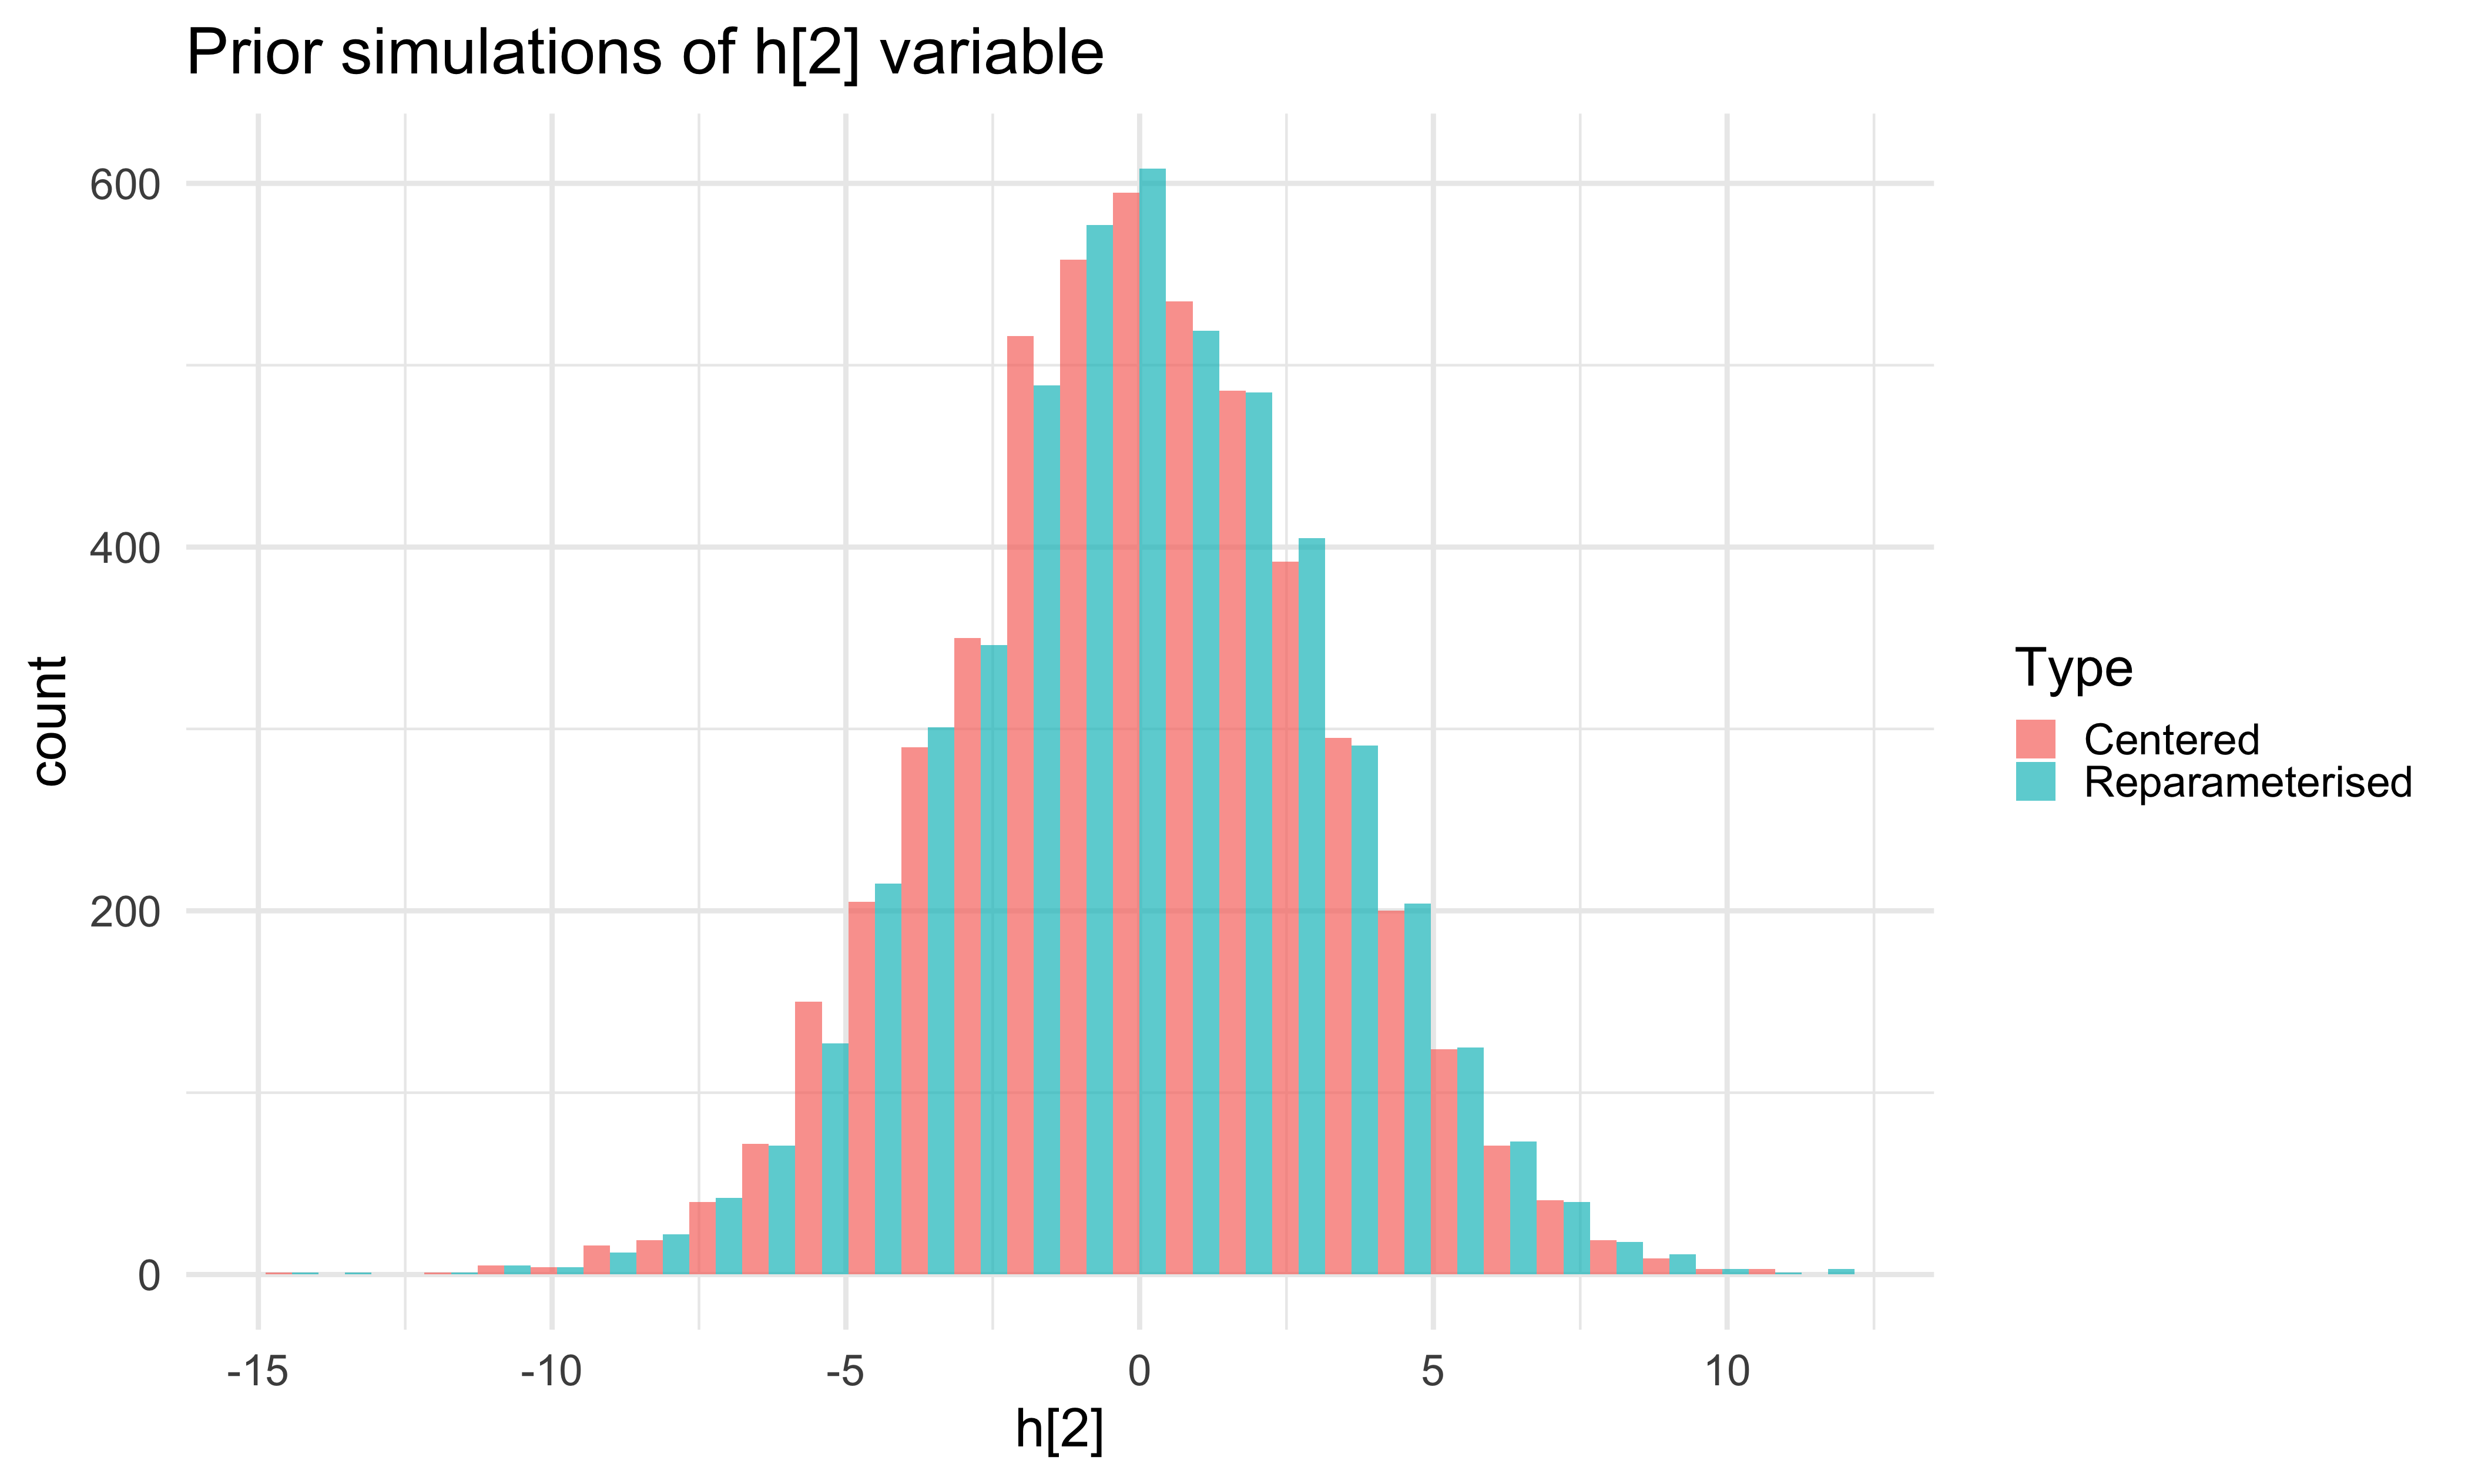
\includegraphics[scale=0.1]{figures/ppc_h2.png}
            \caption{Prior predictive simulation of second state variable from both centered and reparameterised stochastic volatility model. Both models are mathematically equivalent and generate samples from the same data generating process.}
            \label{fig:priorpred}
        \end{figure}
        
        % Emphasise here that different paramterisations of the models are the same model
        % Use a prior predictive check from both paramterisations show that the results are
        % the same



\section{Results}
    1000 and 5000 SBC iterations are run for centered and reparameterised versions of the stochastic volatility model using simulated datasets of 1000 observations. Rank statistic histograms are constructed with 20 bins for the static parameters and the 1st, 500th and 1000th latent state variables. The black horizontal line represents uniformity conditional on the number of bins and SBC iterations. The $\chi^2$ statistic is used to summarise the deviations from uniformity for all state variables since it is unrealistic to visually inspect all the histograms. The SBC algorithm is summarised Algorithm \ref{alg:sbc}:

    \begin{algorithm}
        \caption{SBC}\label{alg:sbc}
        \begin{algorithmic}
        \For{\texttt{i in} $1:1000$}
                \State \text{Draw from joint prior: } $\boldsymbol{\theta}^{sim}_i \sim\pi (\boldsymbol{\theta})$
                \State \text{Simulate dataset with 1000 observations: } $\boldsymbol{y}^{sim}_i \sim p(y|\boldsymbol{\theta}^{sim}_i)$
                \State \text{Draw 999 posterior samples post burn in:} $\{\boldsymbol{\theta}_1,\dots , \boldsymbol{\theta}_{999}\}_i \sim p(\theta | \boldsymbol{y}^{sim}_i)$
                \State \text{Compute rank statistics:} $\boldsymbol{r} = rank(\{\boldsymbol{\theta}_1,\dots , \boldsymbol{\theta}_{999}\}_i, \boldsymbol{\theta}^{sim}_i)$
              \EndFor
        \end{algorithmic}
        \end{algorithm}
        
    \subsection{Hamiltonian Monte Carlo}
    Figure \ref{fig:cphmc1k} and Figure \ref{fig:ncphmc1k} show the SBC results for the centered and reparameterisd model for HMC respectively. Both sets of results display relatively noisy rank statistic estimates with variation around the discrete uniform distribution.

    The centered parameterisation in particular displays a lack of uniformity for $\phi$ and $\sigma^2$. Rank statistics for $\sigma^2$ and $\phi$ show two peaks of either end of the histogram. The posterior estimates of $\sigma^2$ and $\phi$ are \textit{underdispersed} relative to the prior distribution. This implies the posterior geometry of these parameters may be difficult to sample for the HMC algorithm.

    \begin{figure}[H]
        \centering
        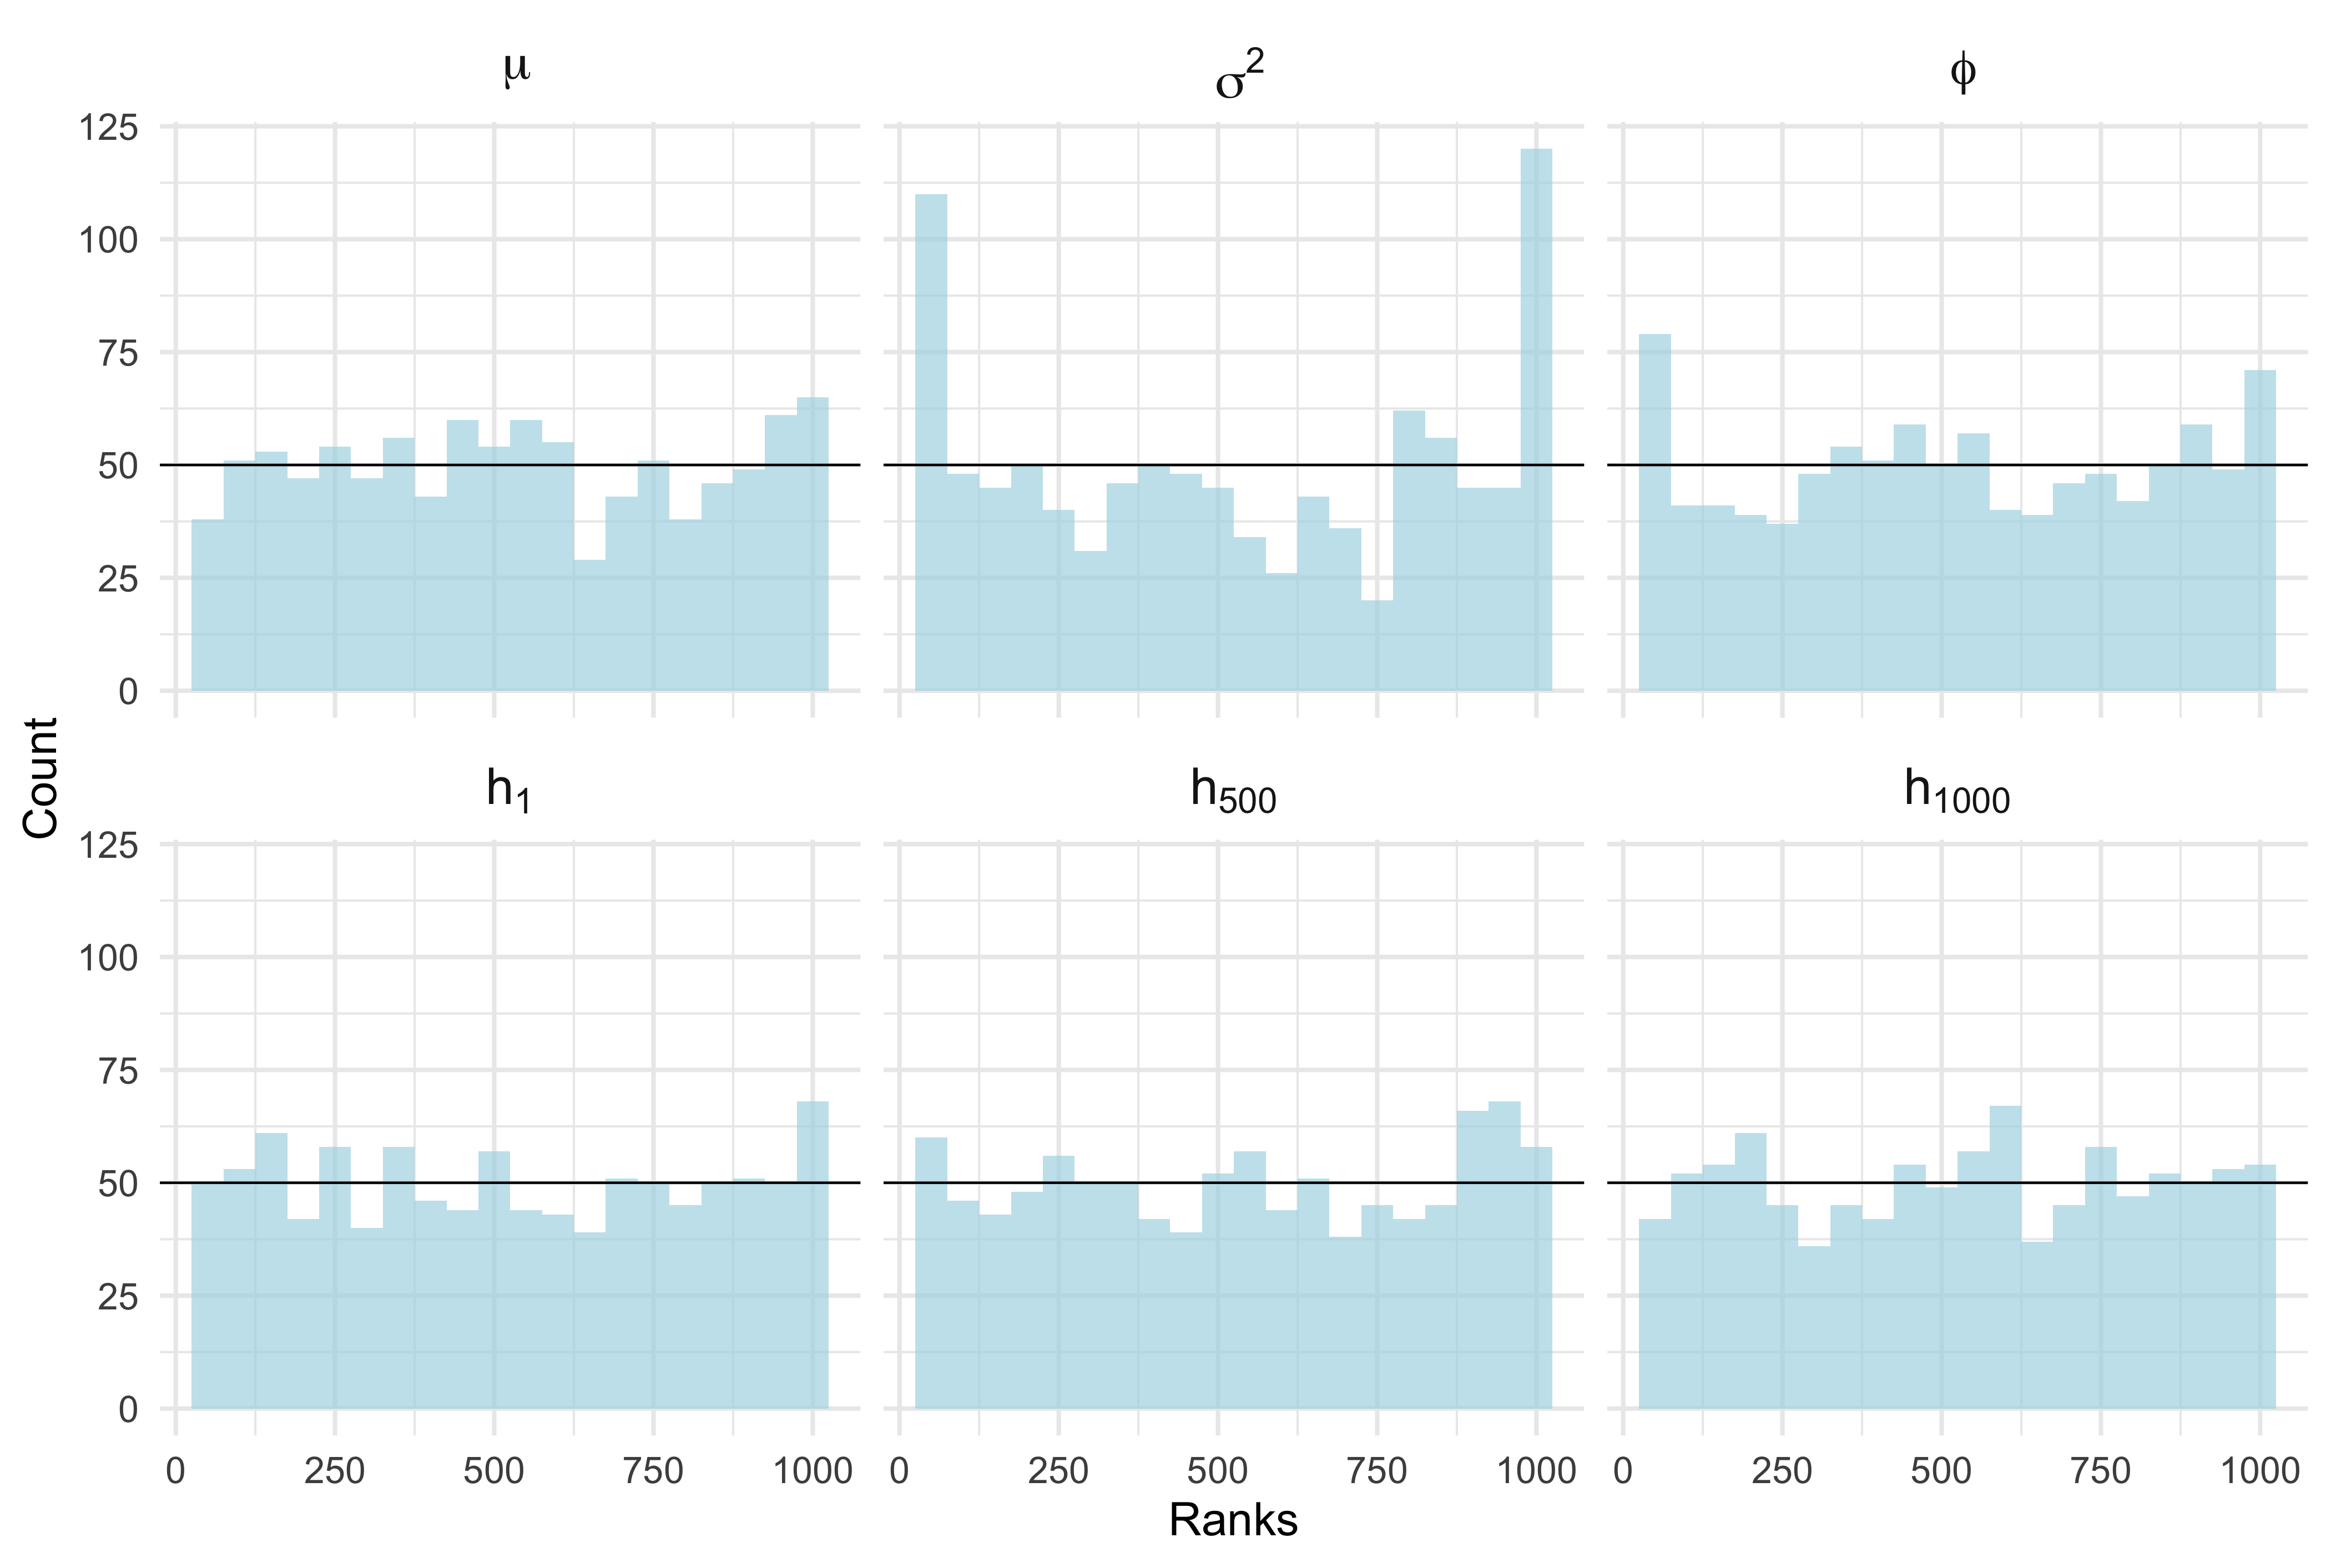
\includegraphics[scale=0.09]{results/hmc_cp_1k.png}
        \caption{1000 SBC iterations for centered model using Hamiltoninan Monte Carlo. Histograms show noisy estimates around uniform distribution. In particular, $\sigma^2$ displays peaks on both ends of the histogram and $\phi$ shows a major on the left hand side. This suggests that the posterior samples of $\sigma^2$ are underdispersed relative to the prior distribution and posterior samples of $\phi$ are over estimating the true parameter.}
        \label{fig:cphmc1k}
    \end{figure} 

    Estimates of $\sigma^2$ and $\phi$ are more uniform under the reparameterised model. Instead, we observe a peak on the left side for the 500th state variable $h_{500}$. Overall the estimates for non centered parameterisation are more favourable. 

    \begin{figure}[H]
        \centering
        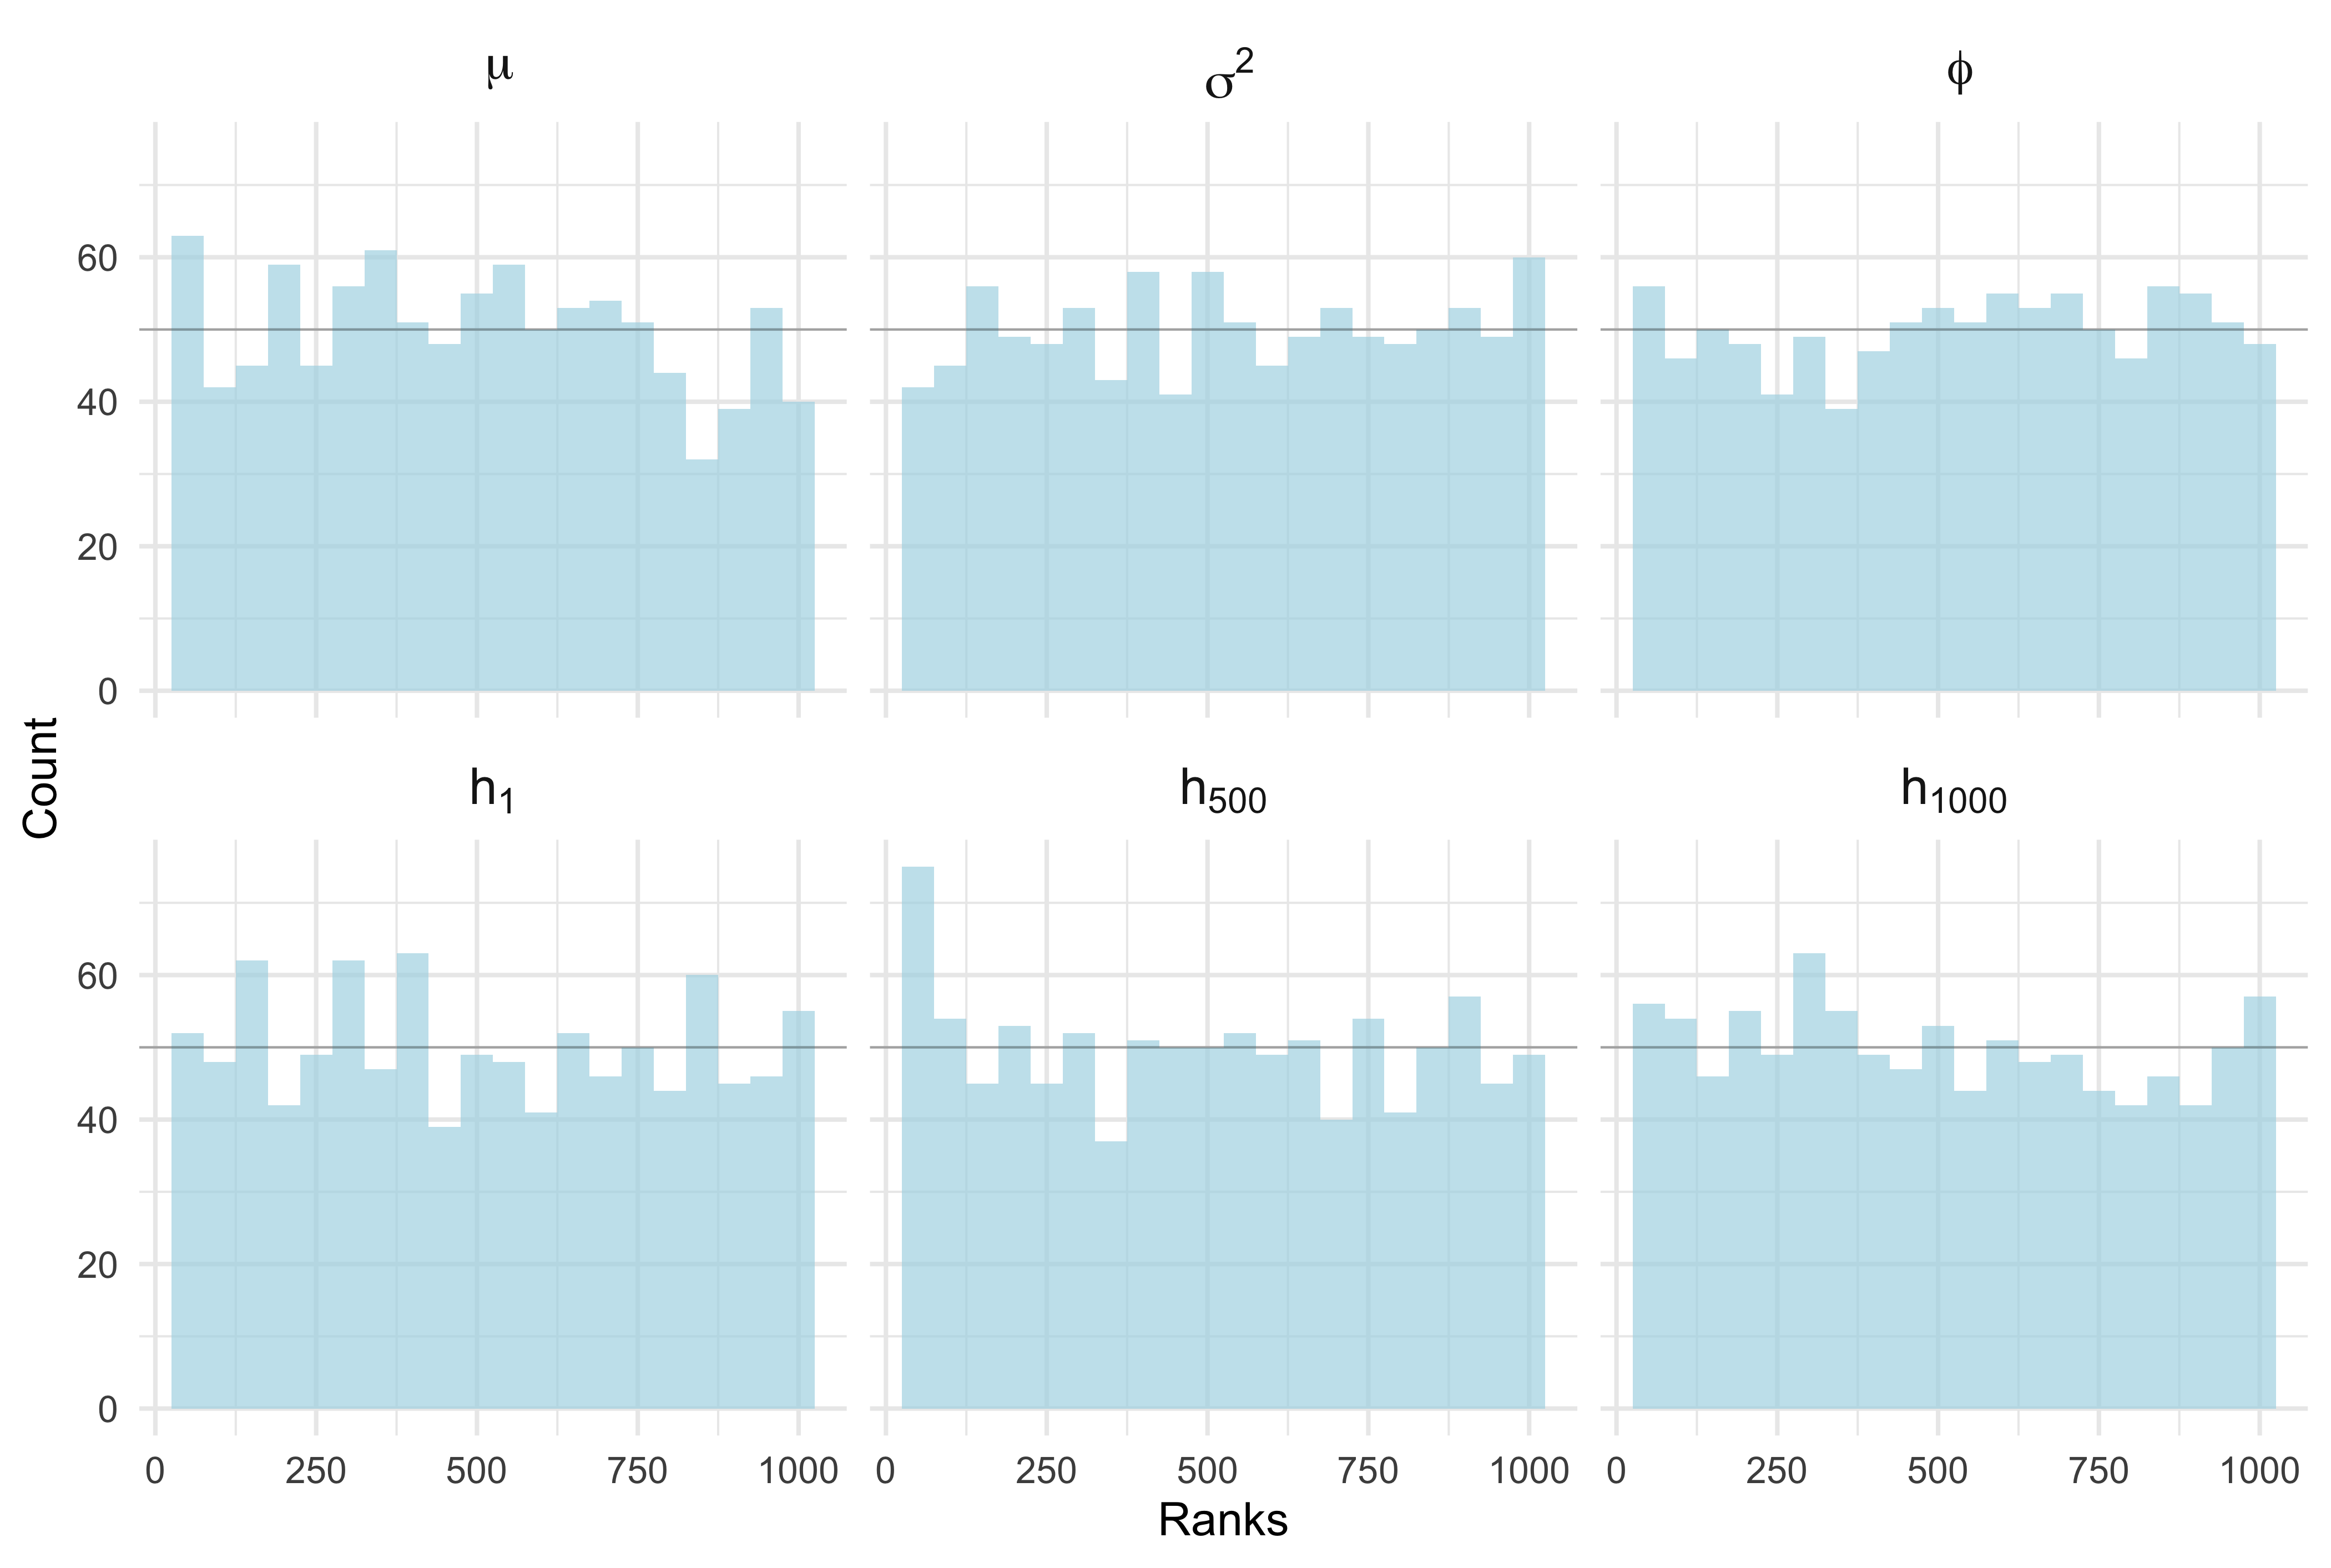
\includegraphics[scale=0.09]{results/hmc_ncp_1k.png}
        \caption{1000 SBC iterations for non centered model using Hamiltonian Monte Carlo. The rank statistic distributions for $\sigma^2$ and $\phi$ have improved. There is some evidence that the posterior of the 500th state variable is overestimating the distribution of its true value.}
        \label{fig:ncphmc1k}
    \end{figure}

    The noisy histogram estimates can be improved by increasing the number of SBC iterations. Figure \ref{fig:cphmc5k} and Figure \ref{fig:ncphmc5k} show the results of the same parameters with 5000 SBC iterations. There is an improvement to the reparameterised model with all histograms looking approximately uniform with much smaller variation around the uniform distribution. 
    
    Centered parameteristion posess similar improvement for $\mu$ and the state variables. However, there are still major peaks at both ends of $\sigma^2$ and $\phi$ suggesting underdispersion of the posterior estimates relative to the prior distribution.

    These results suggests that HMC struggles to sample some parameters from the centered parameteristion of the stochastic volatility model. The reparameterised model possess stronger evidence of calibration for the parameters examined, implying more reliable and consistent inference.

    \begin{figure}[H]
        \centering
        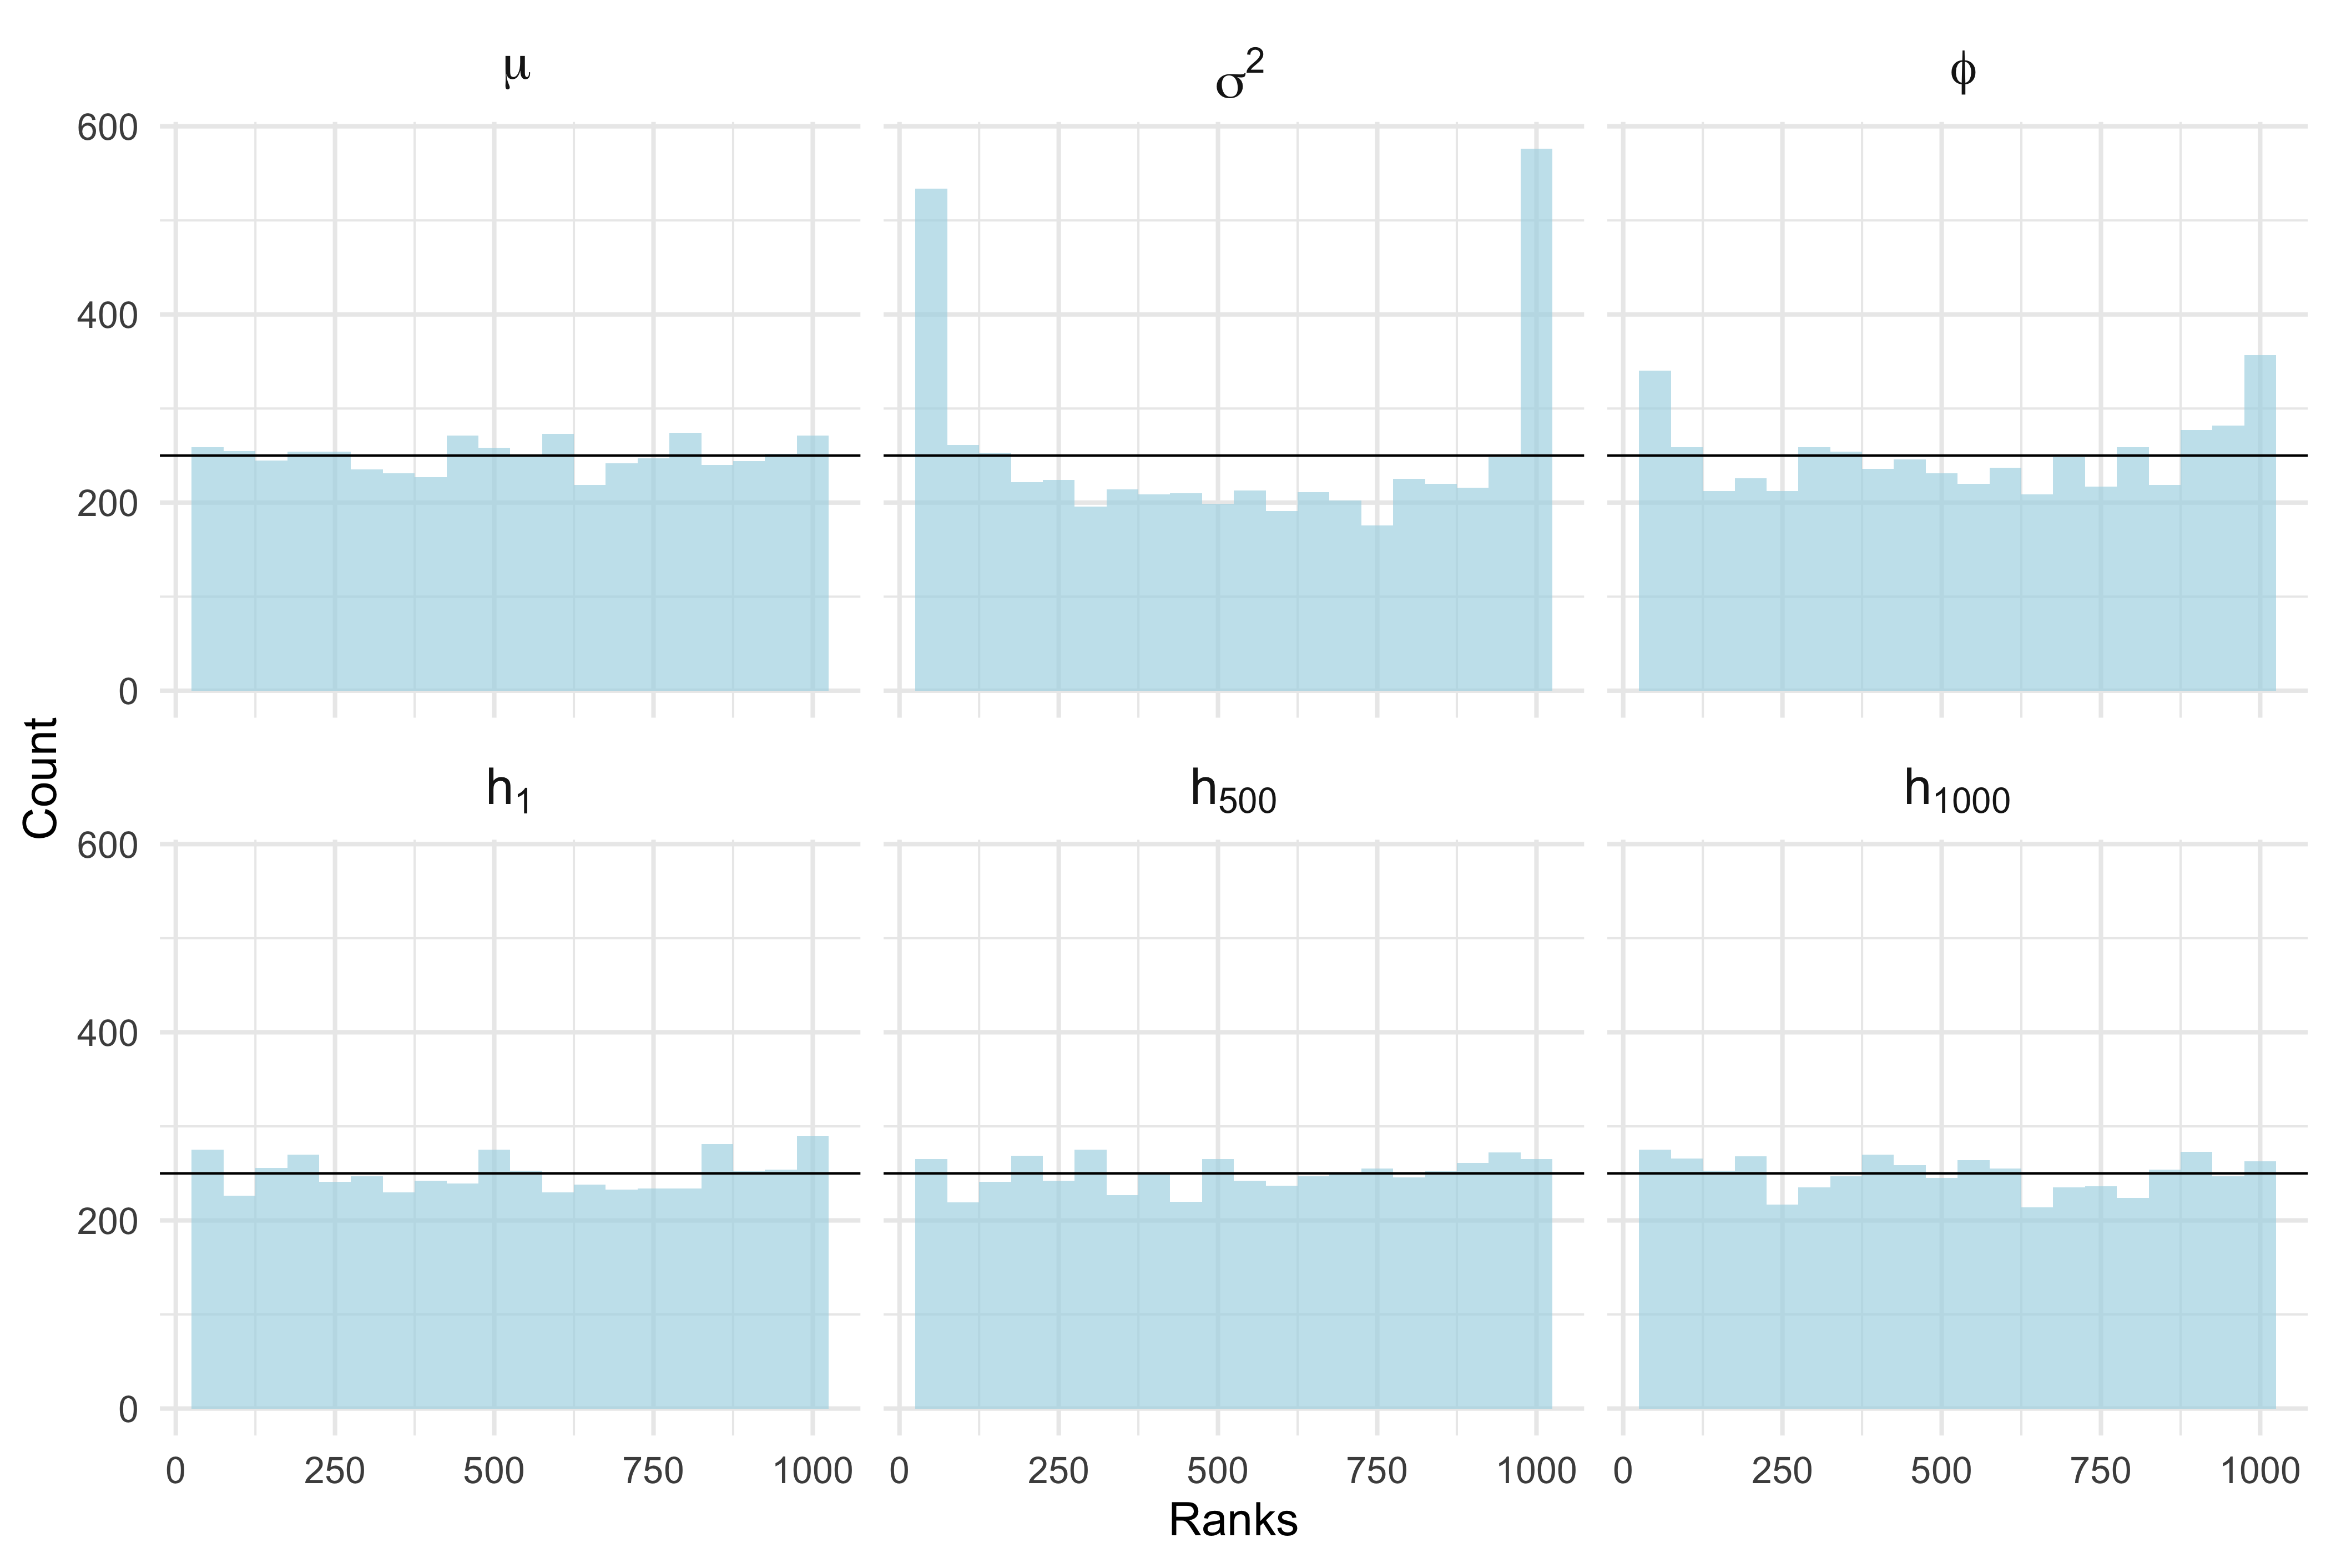
\includegraphics[scale=0.09]{results/hmc_cp_5k.png}
        \caption{5000 SBC iterations for centered model using Hamiltoninan Monte Carlo. $\mu$ and the state parameters look approximately uniform. $\sigma^2$ still has major peaks on both the left and right hand side indicating underdispersion relative to the prior distribution. $\phi$ exhibits a similar shape to $\sigma^2$ although the peaks are much smaller.}
        \label{fig:cphmc5k}
    \end{figure}

    \begin{figure}[H]
        \centering
        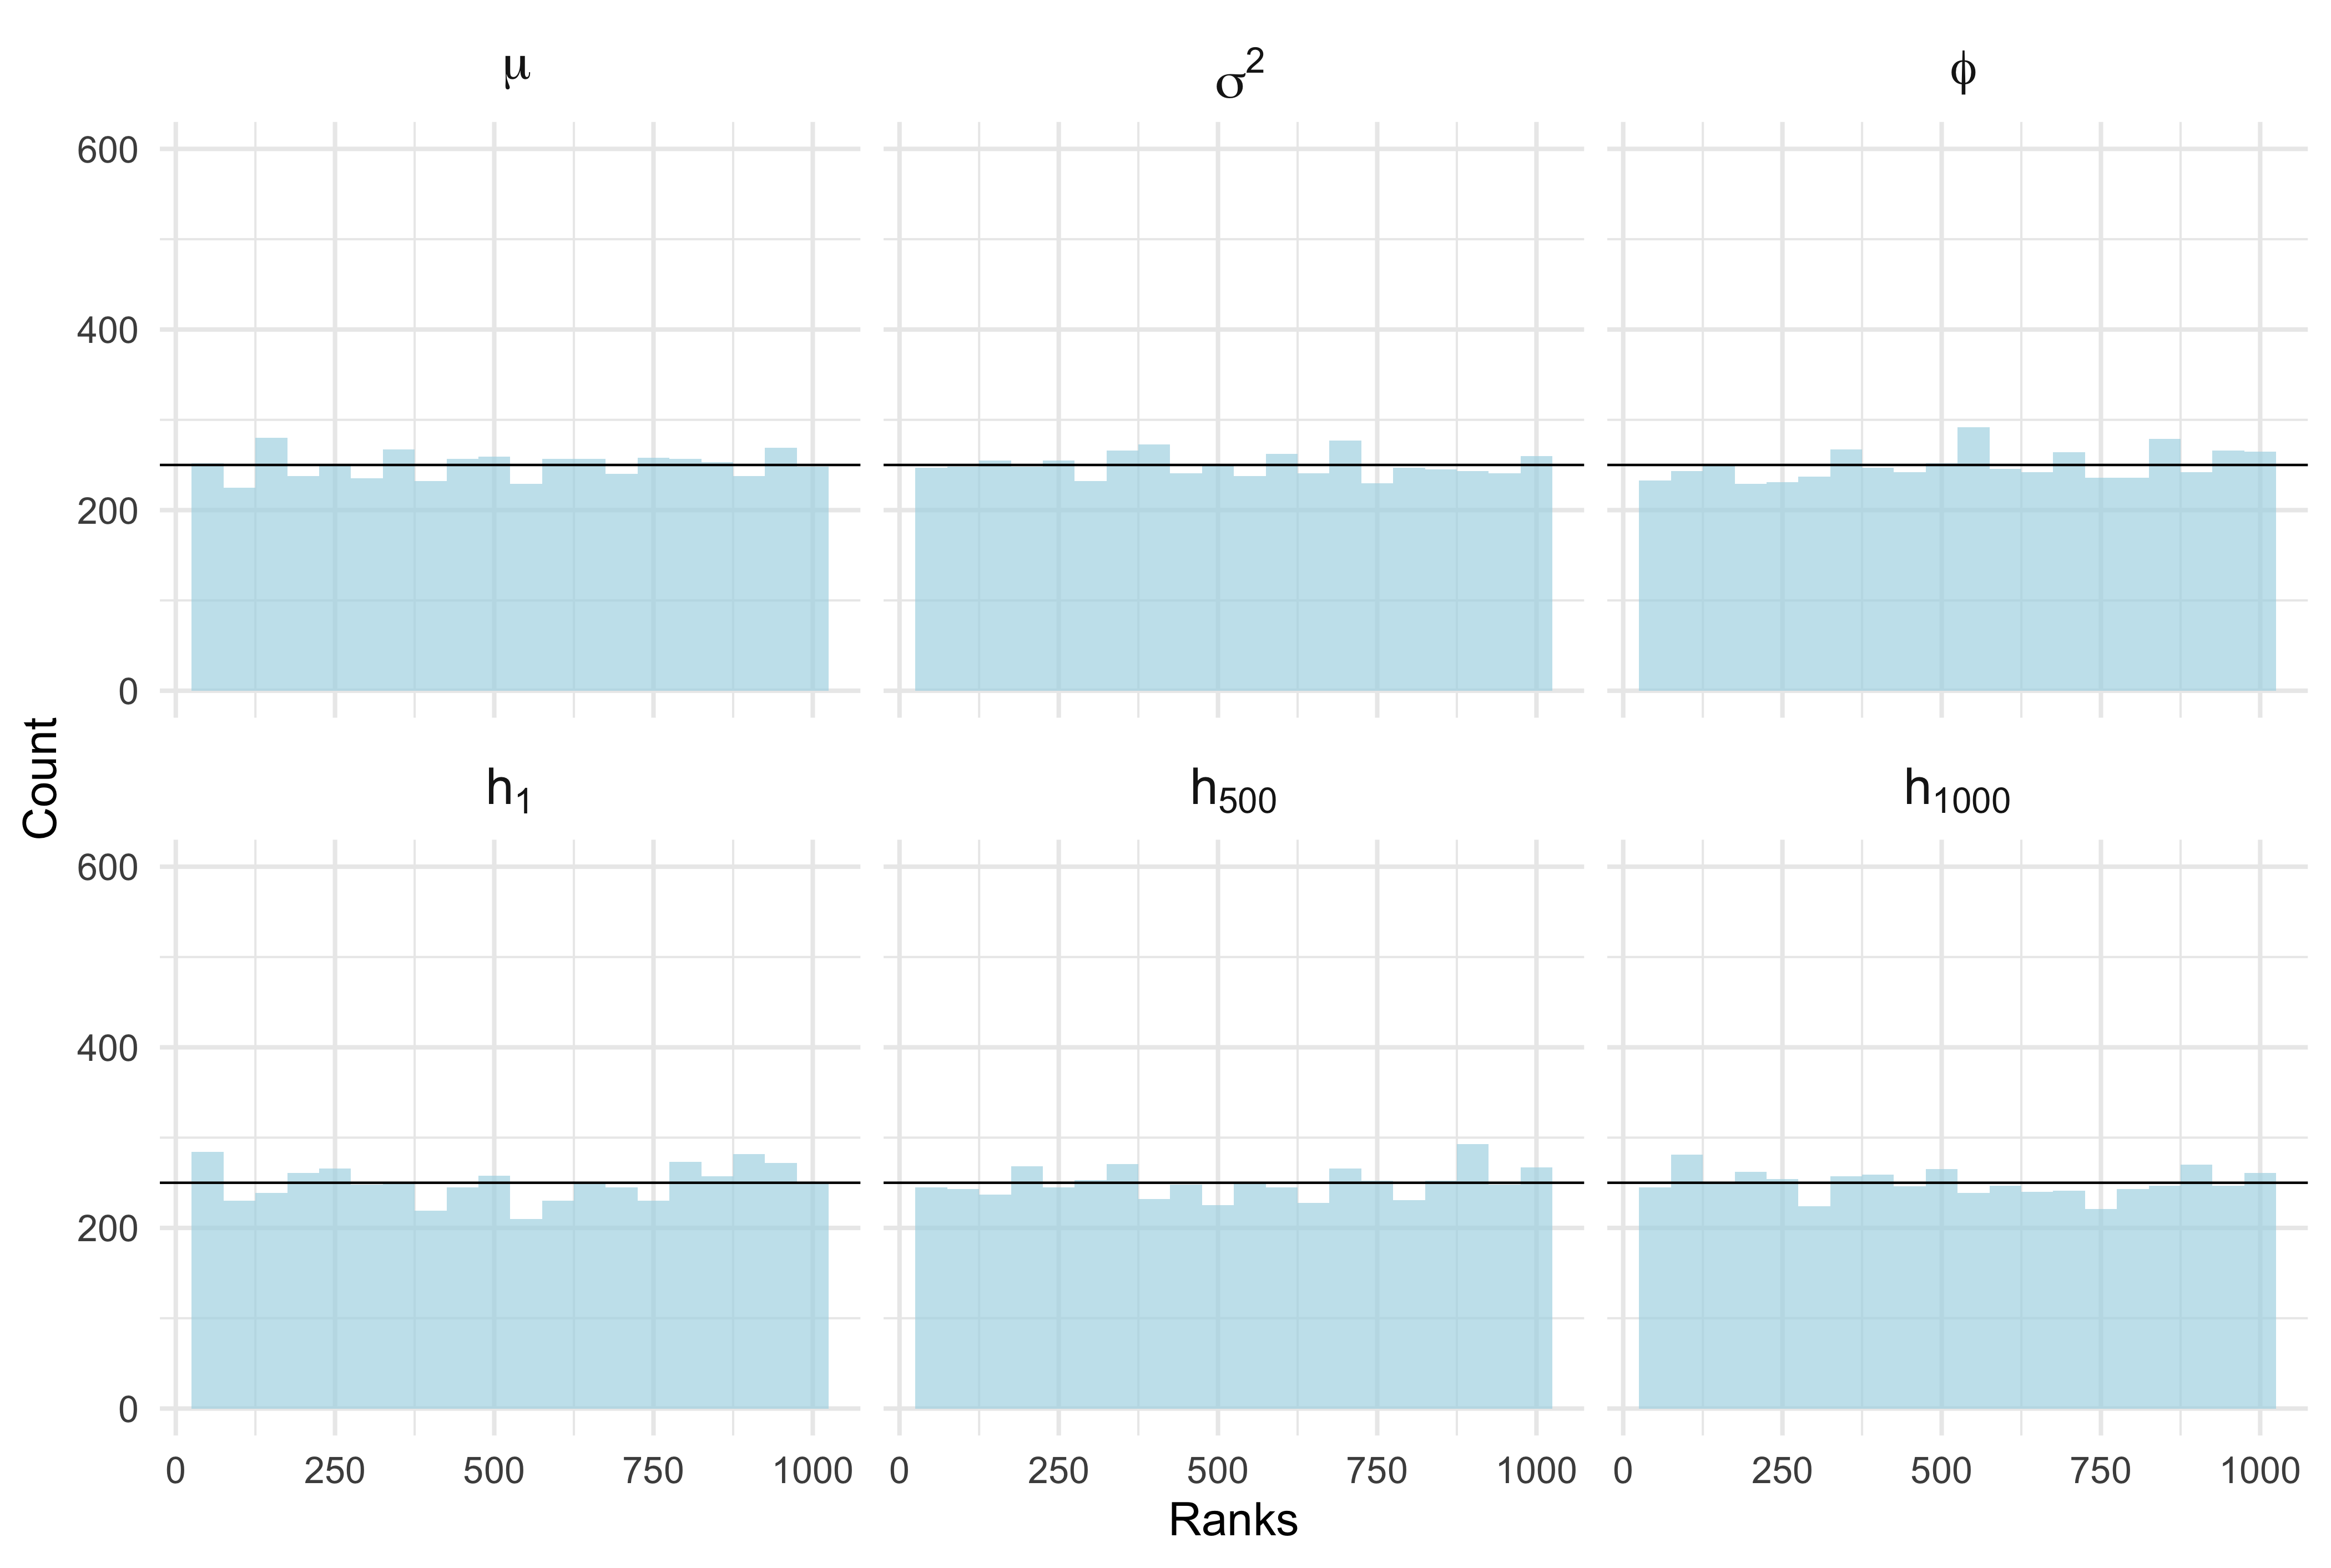
\includegraphics[scale=0.09]{results/hmc_ncp_5k.png}
        \caption{5000 SBC iterations for reparameterised model using Hamiltoninan Monte Carlo. Parameters display uniformity with less noise around the true uniform value. This suggests that the HMC algorithm is returning the correct posterior estimates for the selected parameters.}
        \label{fig:ncphmc5k}
    \end{figure}

    Additionally, HMC struggles to generate efficient posterior samples from the centered parameterisation of the stochastic volatility model. Figure \ref{fig:hmcess} and Table \ref{tab:hmcess} summarises the distribution of ESS for the static parameters after 5000 SBC iterations. The non centered model appears to generate independent samples much more efficiently than the centered model. This is consistent with HMC struggliing to sample overall from the posteriors of $\sigma^2$ and $\phi$.

    \begin{figure}[H]
        \centering
        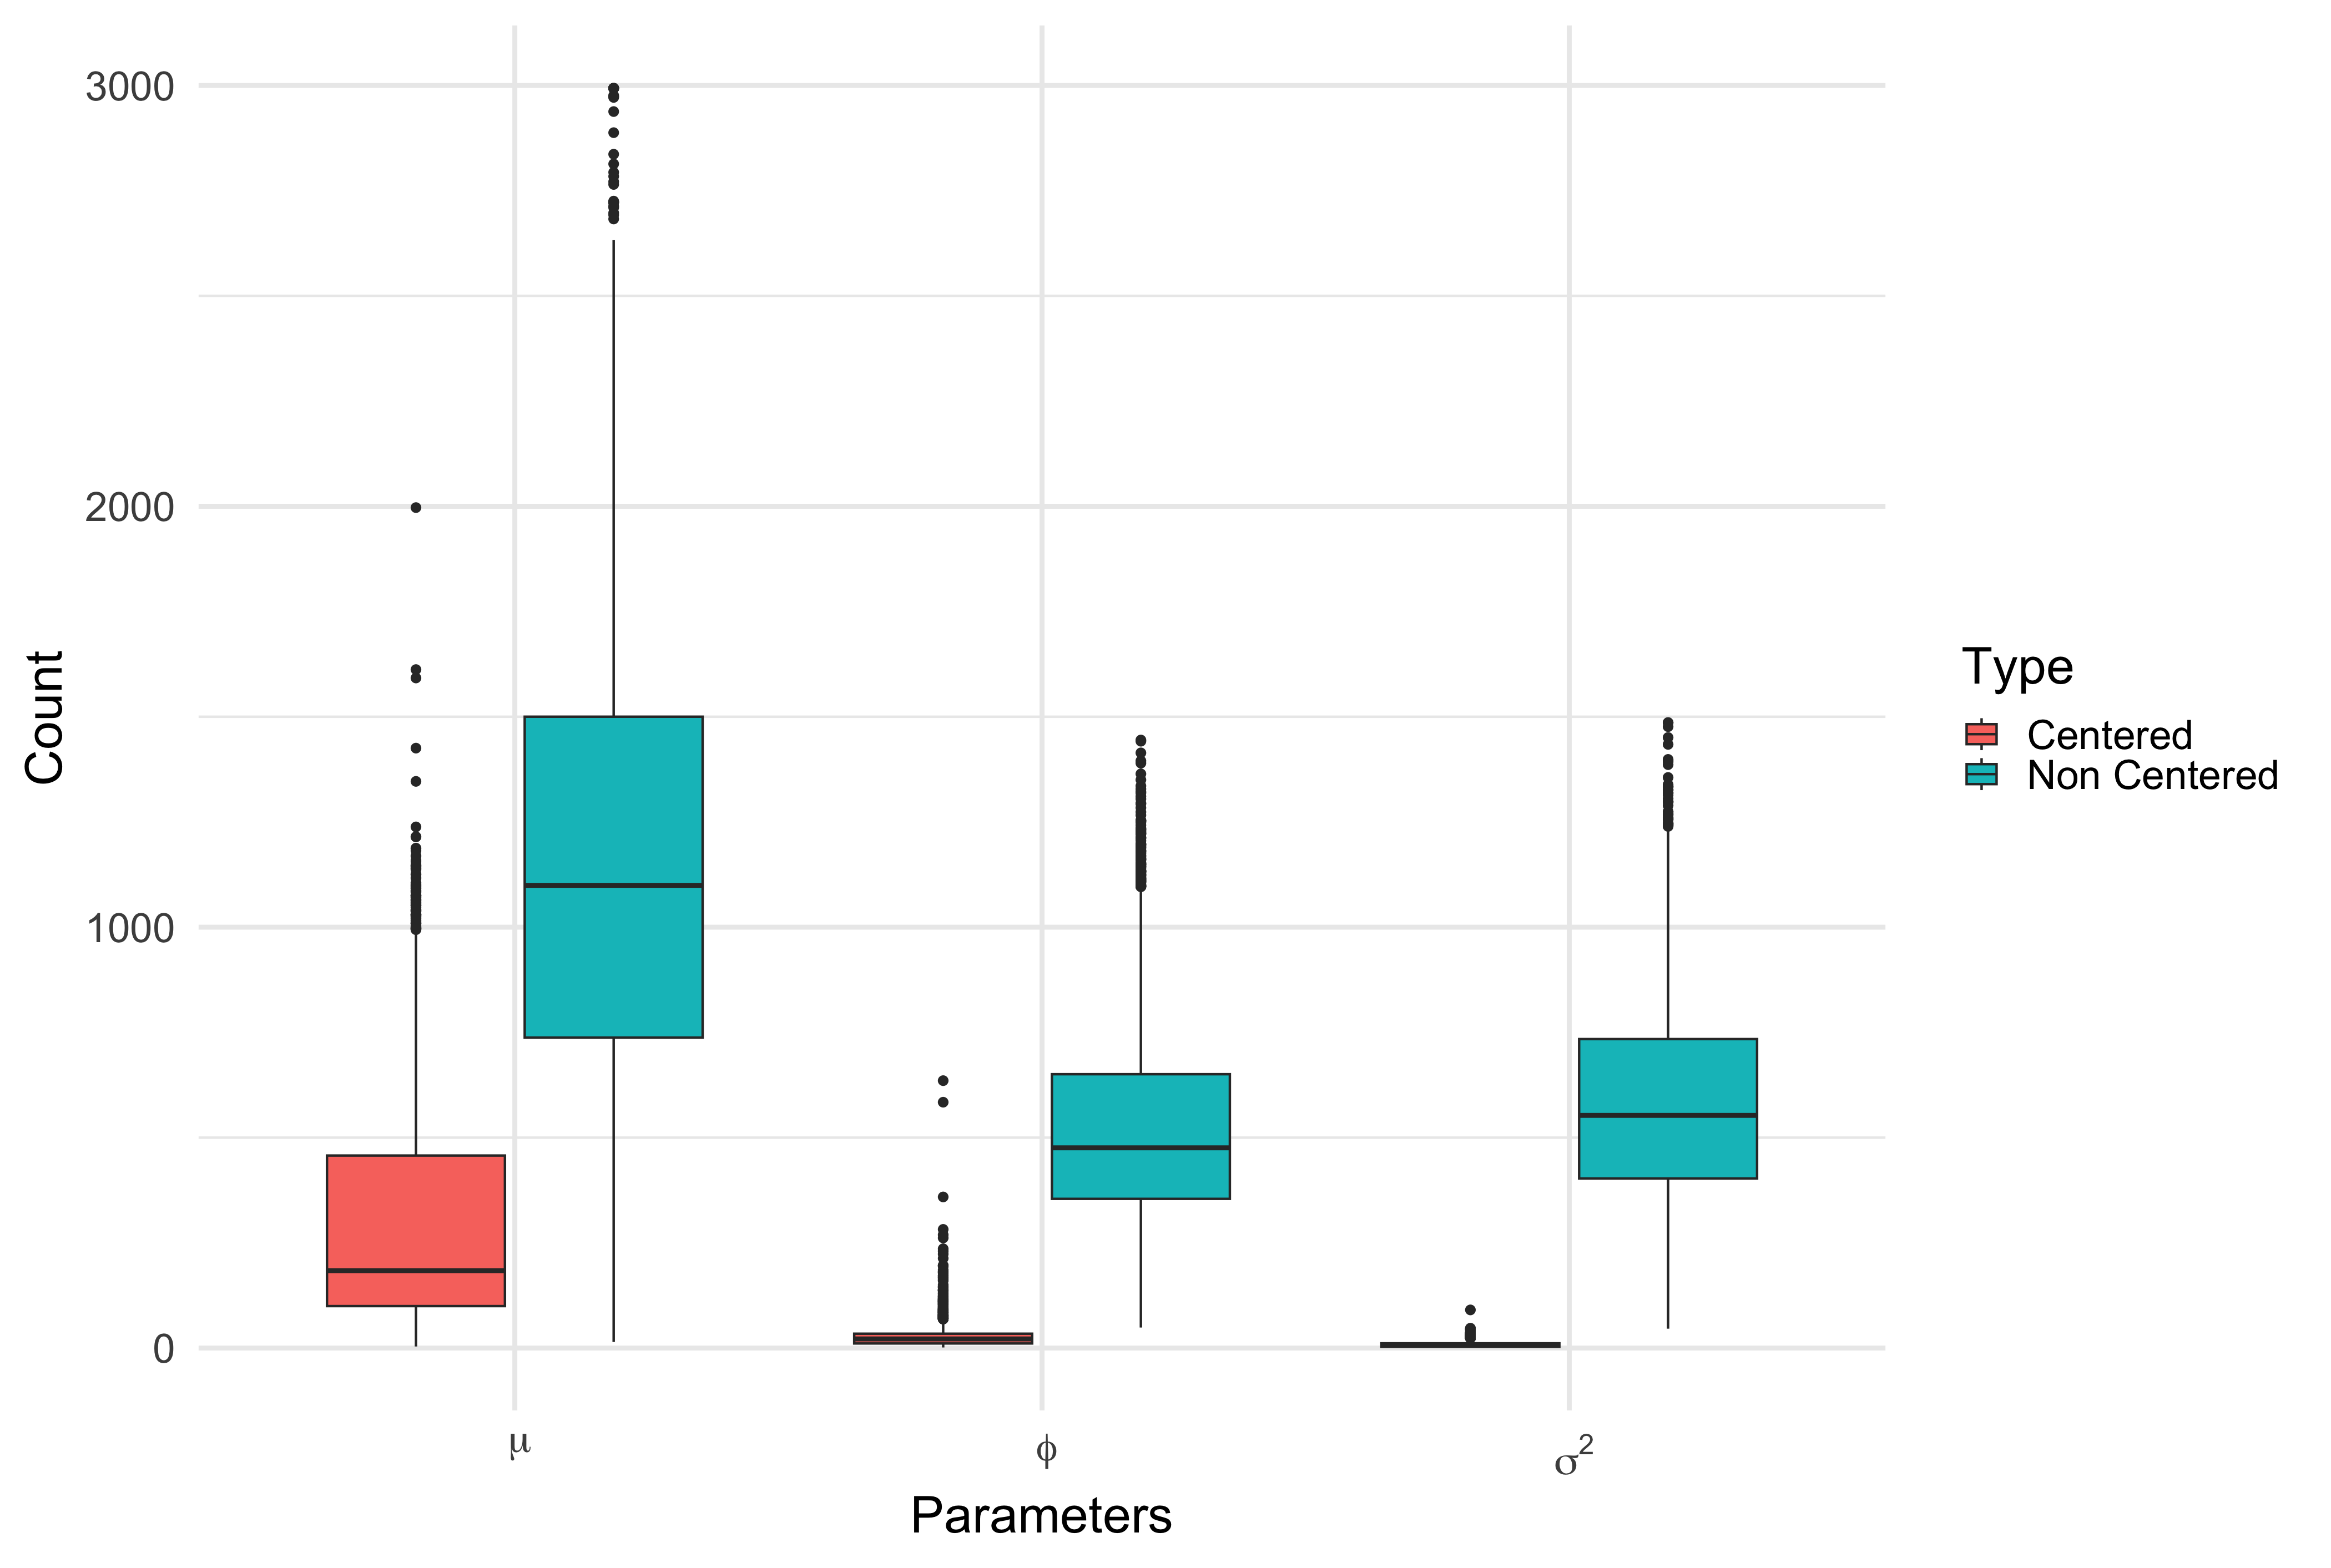
\includegraphics[scale=0.09]{results/hmc_ess.png}
        \caption{Effective sample sizes for static parameters after 5000 iterations of SBC and 1000 post warmup samples for Hamiltoninan Monte Carlo. The centered parameterisation struggles to generate independent samples for $\sigma^2$ and $\phi$. Non parameterisation demonstrates much more efficient sampling behaviour.}
        \label{fig:hmcess}
    \end{figure}

    \begin{table}[H]
        \centering
        \begin{tabular}{|c|c|c|c|c|c|c|c|} \hline 
        Parameter &  Type&Min& q25&  Median& Mean & q75&Max\\ \hline 
        $\mu$&  Centered&3.79 & 99.7 & 184. & 305. & 457. & 1997.  \\
     $\mu$&  Reparam&14.5 & 738. & 1099. & 1143. & 1500. & 2993.  \\\hline 
     $\phi$&  Centered&1.44 & 11.0 & 21.7 & 26.3 & 34.1 & 635.  \\
     $\phi$&  Reparam&48.8 & 355. & 476. & 521. & 651. & 1445.   \\ \hline 
     $\sigma^2$&  Centered& 1.17 & 2.99 & 7.04 & 8.05 & 11.3 & 90.7 \\ 
     $\sigma^2$&  Reparam&46.1 & 403. & 553. & 585. & 734. & 1486. \\ \hline
        \end{tabular}
        \caption{HMC: ESS for centered and reparameterised stochastic volatility model.}
        \label{tab:hmcess}
    \end{table}

    \subsection{Gaussian Mixture Approximation}
    The Gaussian Mixture Approximation is run with the first 10,000 samples discarded as burnin (following the method of \citet{kim1998stochastic}). However, unlike KSC who take 750,000 posterior draws from the model, the number of posterior samples taken as part of the SBC procedure is 9,999. Taking 750,000 draws from the Gaussian mixture approximation would lead to issues due to disk space limitations and computational resources required to run SBC. Furthermore, the number of posterior samples is larger than the 999 taken for the SBC experiment run for Hamiltonian Monte Carlo. Earlier experiments attempted 999 post burn in draws for the Gaussian approximation, however there are concerns that such a short chain would not have converged onto the target posterior distribution. Therefore 9,999 draws was chosen as a compromise under both constraints. 

    The both the centered and reparameterised Gaussian mixture model contains issues with calibration. Figure \ref{fig:cpksc1k} presents the results from the centered model. There is a lack of uniformity across all parameters. In particular, there is a large bias on the left hand side for $\mu$ and the 1st and 500th latent state variables. There is also a bias on the right hand hand side of $\phi$. This suggests overestimation and underestimation of the prior distribution respectively. $\sigma^2$ and the 1000th latent state don't appear to be uniform although this may be due to noisy estimates.

    \begin{figure}[H]
        \centering
        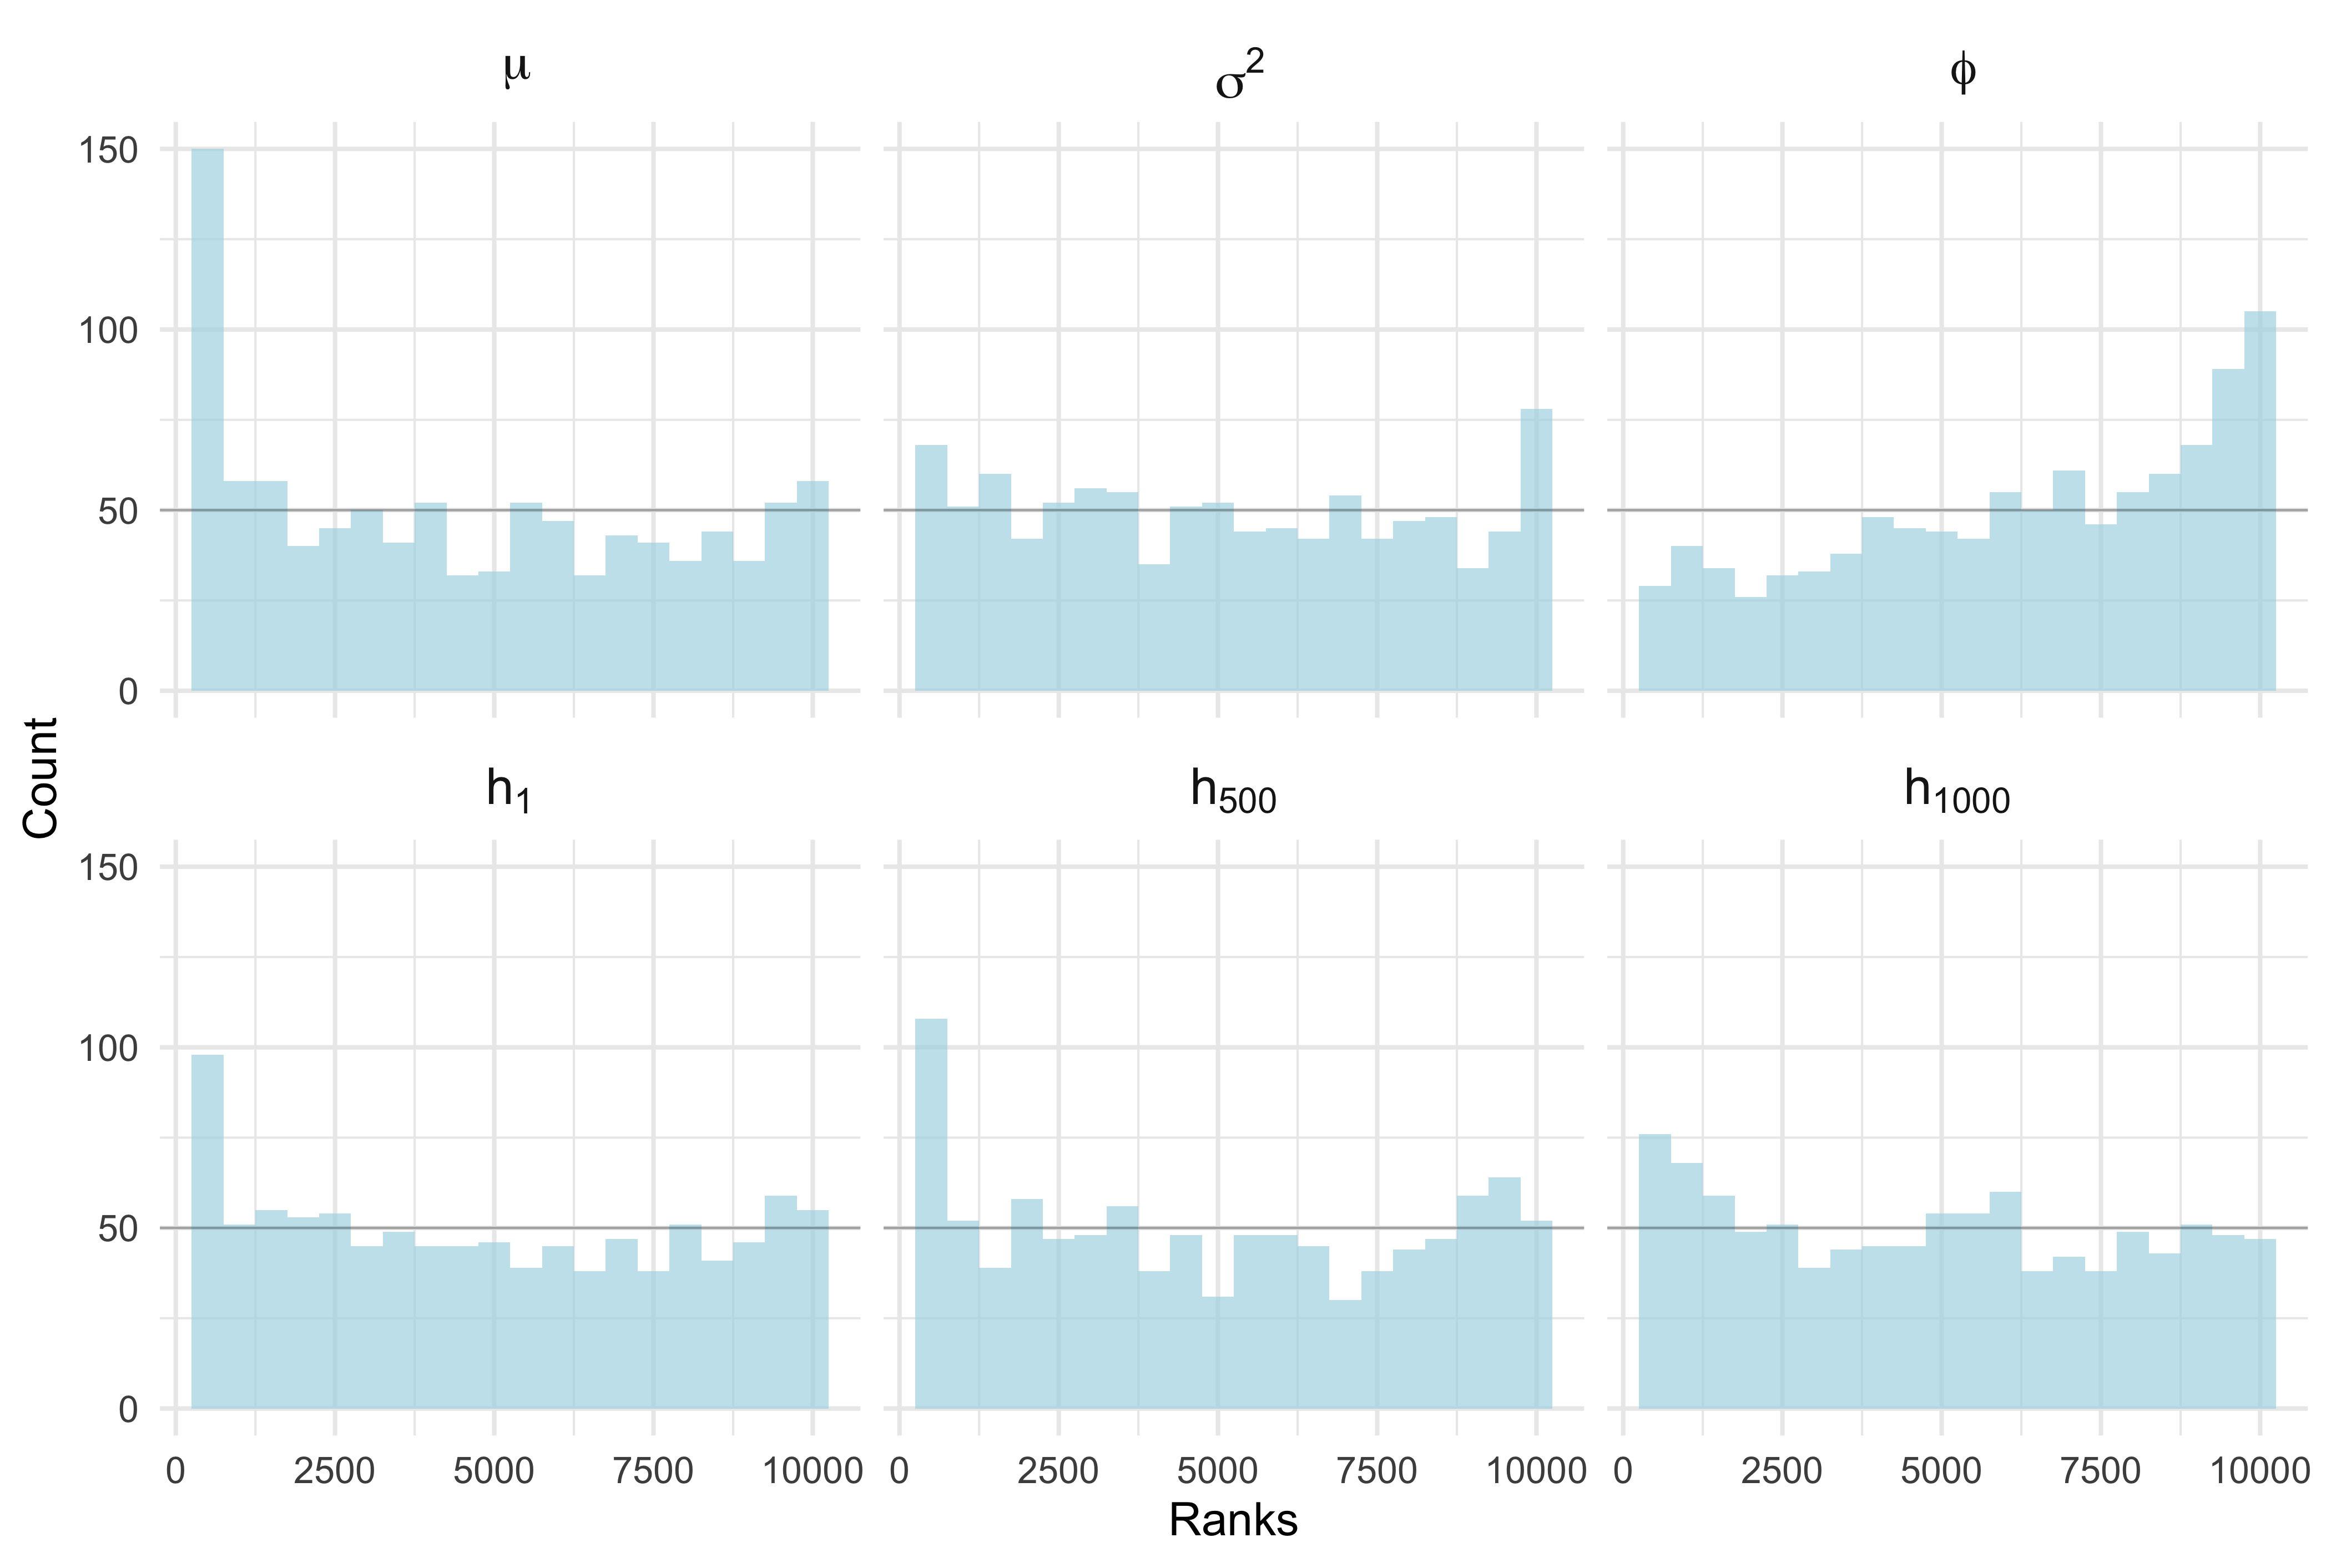
\includegraphics[scale=0.1]{results/ksc_cp_1k.png}
        \caption{1000 SBC iterations for centered Gaussian mixture approximation model. The rank statistics for all the selected parameters display a lack of uniformity. $\mu$ has a large left peak suggesting the algorithm is over estimating the true parameter. The converse can be said about $\phi$ which possesses a peak on the right hand side which implies underestimation of the true parameter. 1st and 500th latent state variables also appear to be over estimating the true value.}
        \label{fig:cpksc1k}
    \end{figure}

    The non centered model in location exhibits larger issues in calibration as shown in Figure \ref{fig:ncpksc1k}. Each histogram exhibits major peaks at one or both ends of the histgoram suggesting major issues in the sampler returning correct posterior estimates. The lack of uniformity for this model is distinctly due to a different shape. Whereas the lack of uniformity for some of the centered SBC results (for KSC) with 1000 iterations may be due to noisy estimates. 

    \begin{figure}[H]
        \centering
        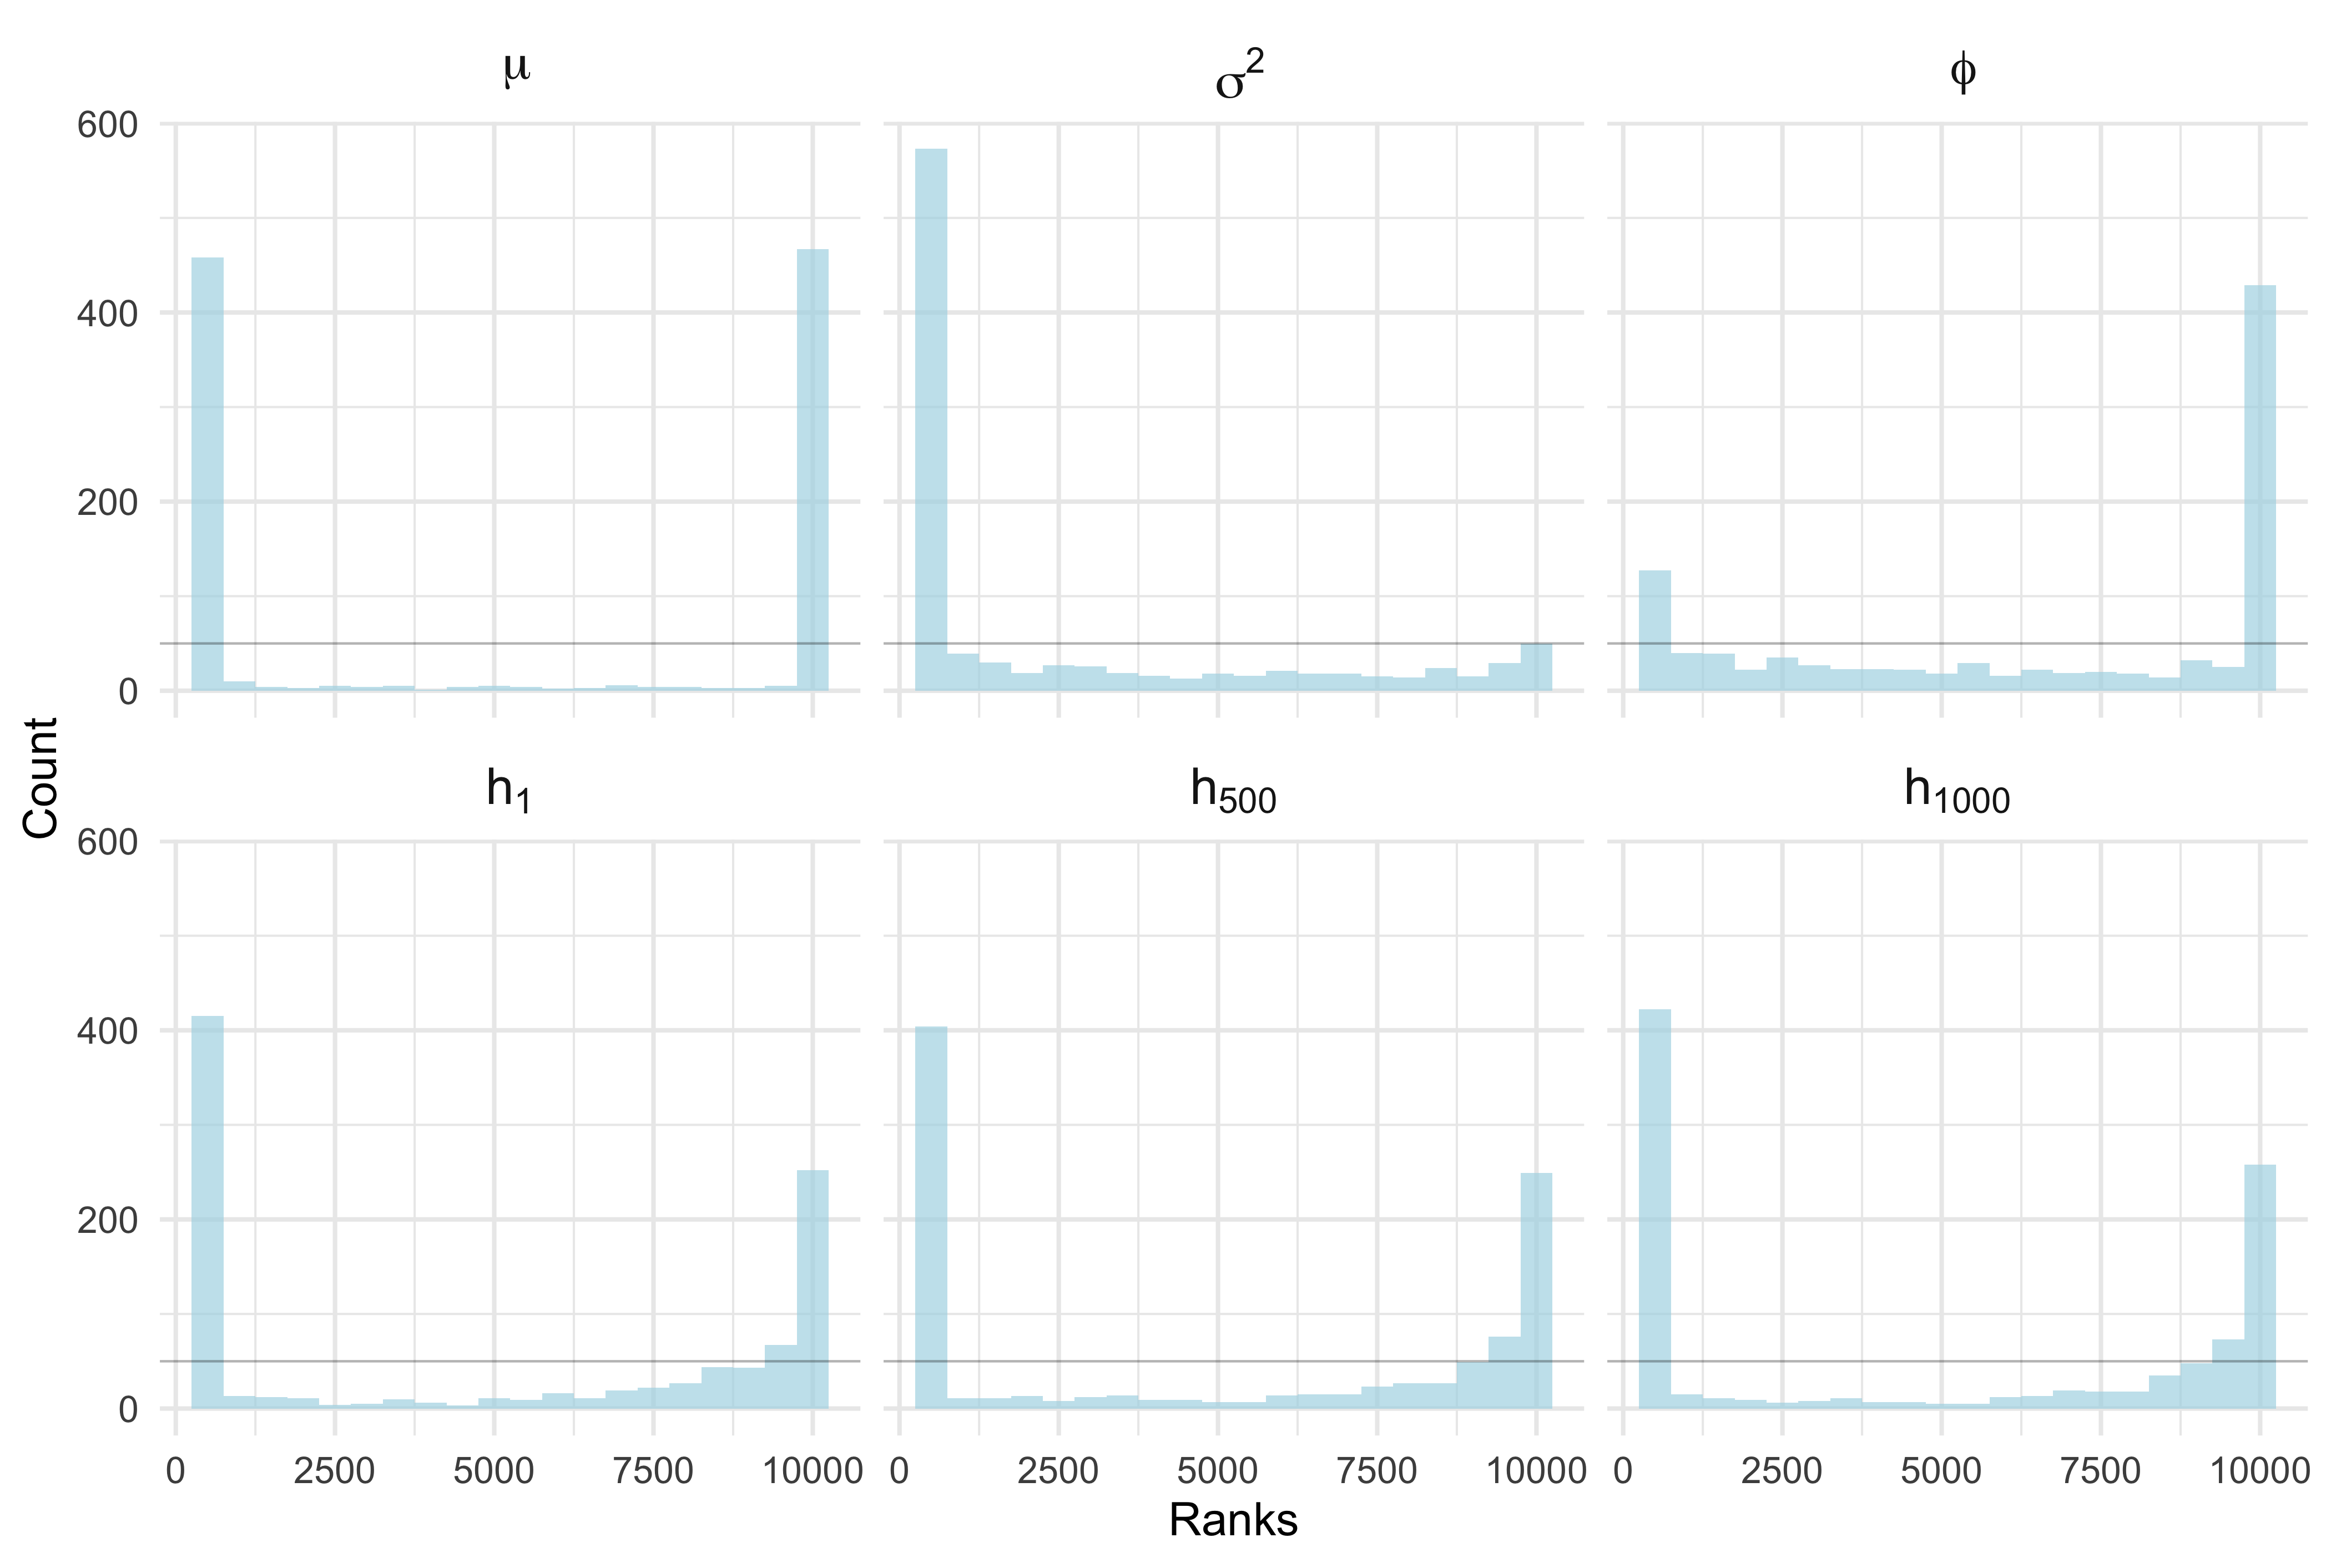
\includegraphics[scale=0.1]{results/ksc_ncp_1k.png}
        \caption{1000 SBC iterations for non centered in location Gaussian mixture approximation model. The rank statistics for all selected parameters are non uniform in shape. The KSC bespoke MCMC struggles to return the correct posteriors for this parametersation of the model.}
        \label{fig:ncpksc1k}
    \end{figure}

    Increasing the SBC iterations to 5000 does not improve the results for either parametersation. $\sigma^2$ contain arguably less noisy estimates around the uniform distribution in the centered parametersation (although there may be evidence of a slight right bias). The skewed shapes of $\mu$ and $\phi$ adds further evidence that the sampling strategy is not returning the correct posterior estimates. All latent state variables appear to have a left side bias. This can be seen in Figure \ref{fig:cpksc5k}.

    Figure \ref{fig:ncpksc5k} shows no improvement to calibration results. The issues in calibration observed in Figure \ref{fig:ncpksc1k} are not due to noisy estimates and are likely the result of problems in the MCMC algorithm and model specification. Applying this parametersation and MCMC on real data will on balance produce incorrect posterior estimates. 

    \begin{figure}[H]
        \centering
        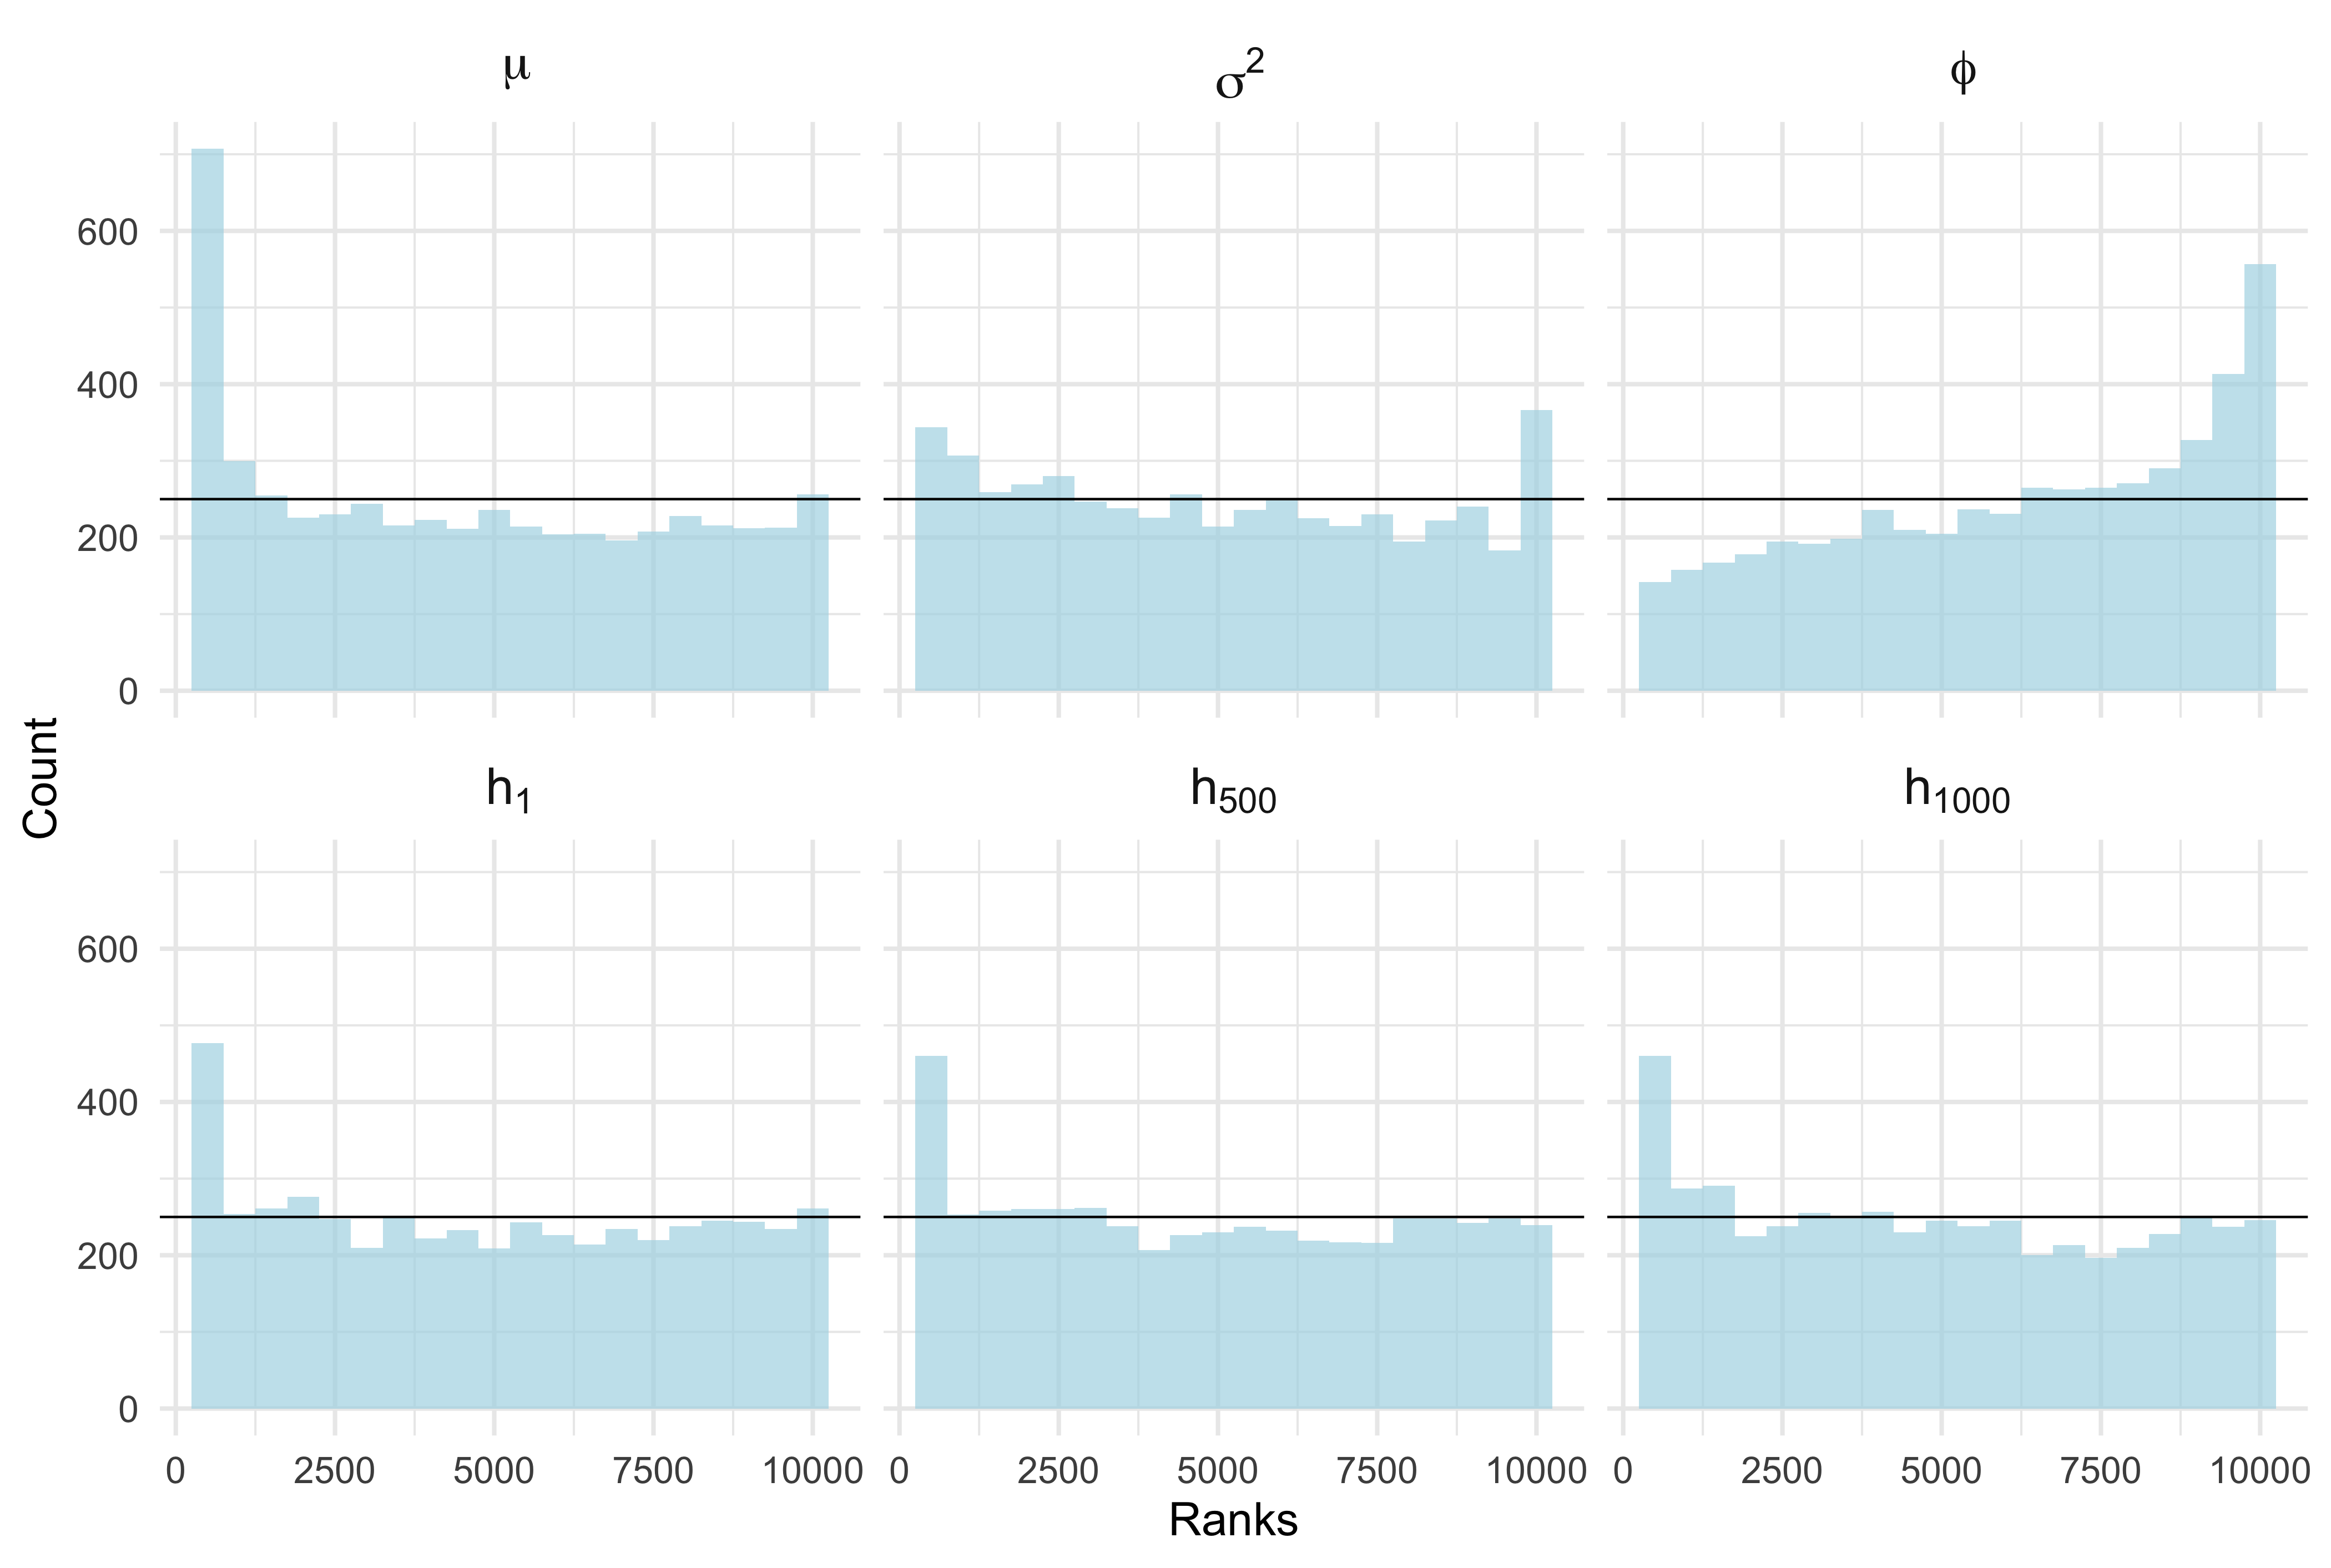
\includegraphics[scale=0.09]{results/ksc_cp_5k.png}
        \caption{5000 SBC iterations for centered Gaussian mixture approximation model. Estimates for $\sigma^2$ may have marginally improved around the uniformity there is still evidence of a ride side bias. There is no improvement in $\mu$ or $\phi$ and all latent state variables appear to have a left side bias.}
        \label{fig:cpksc5k}
    \end{figure}

    \begin{figure}[H]
        \centering
        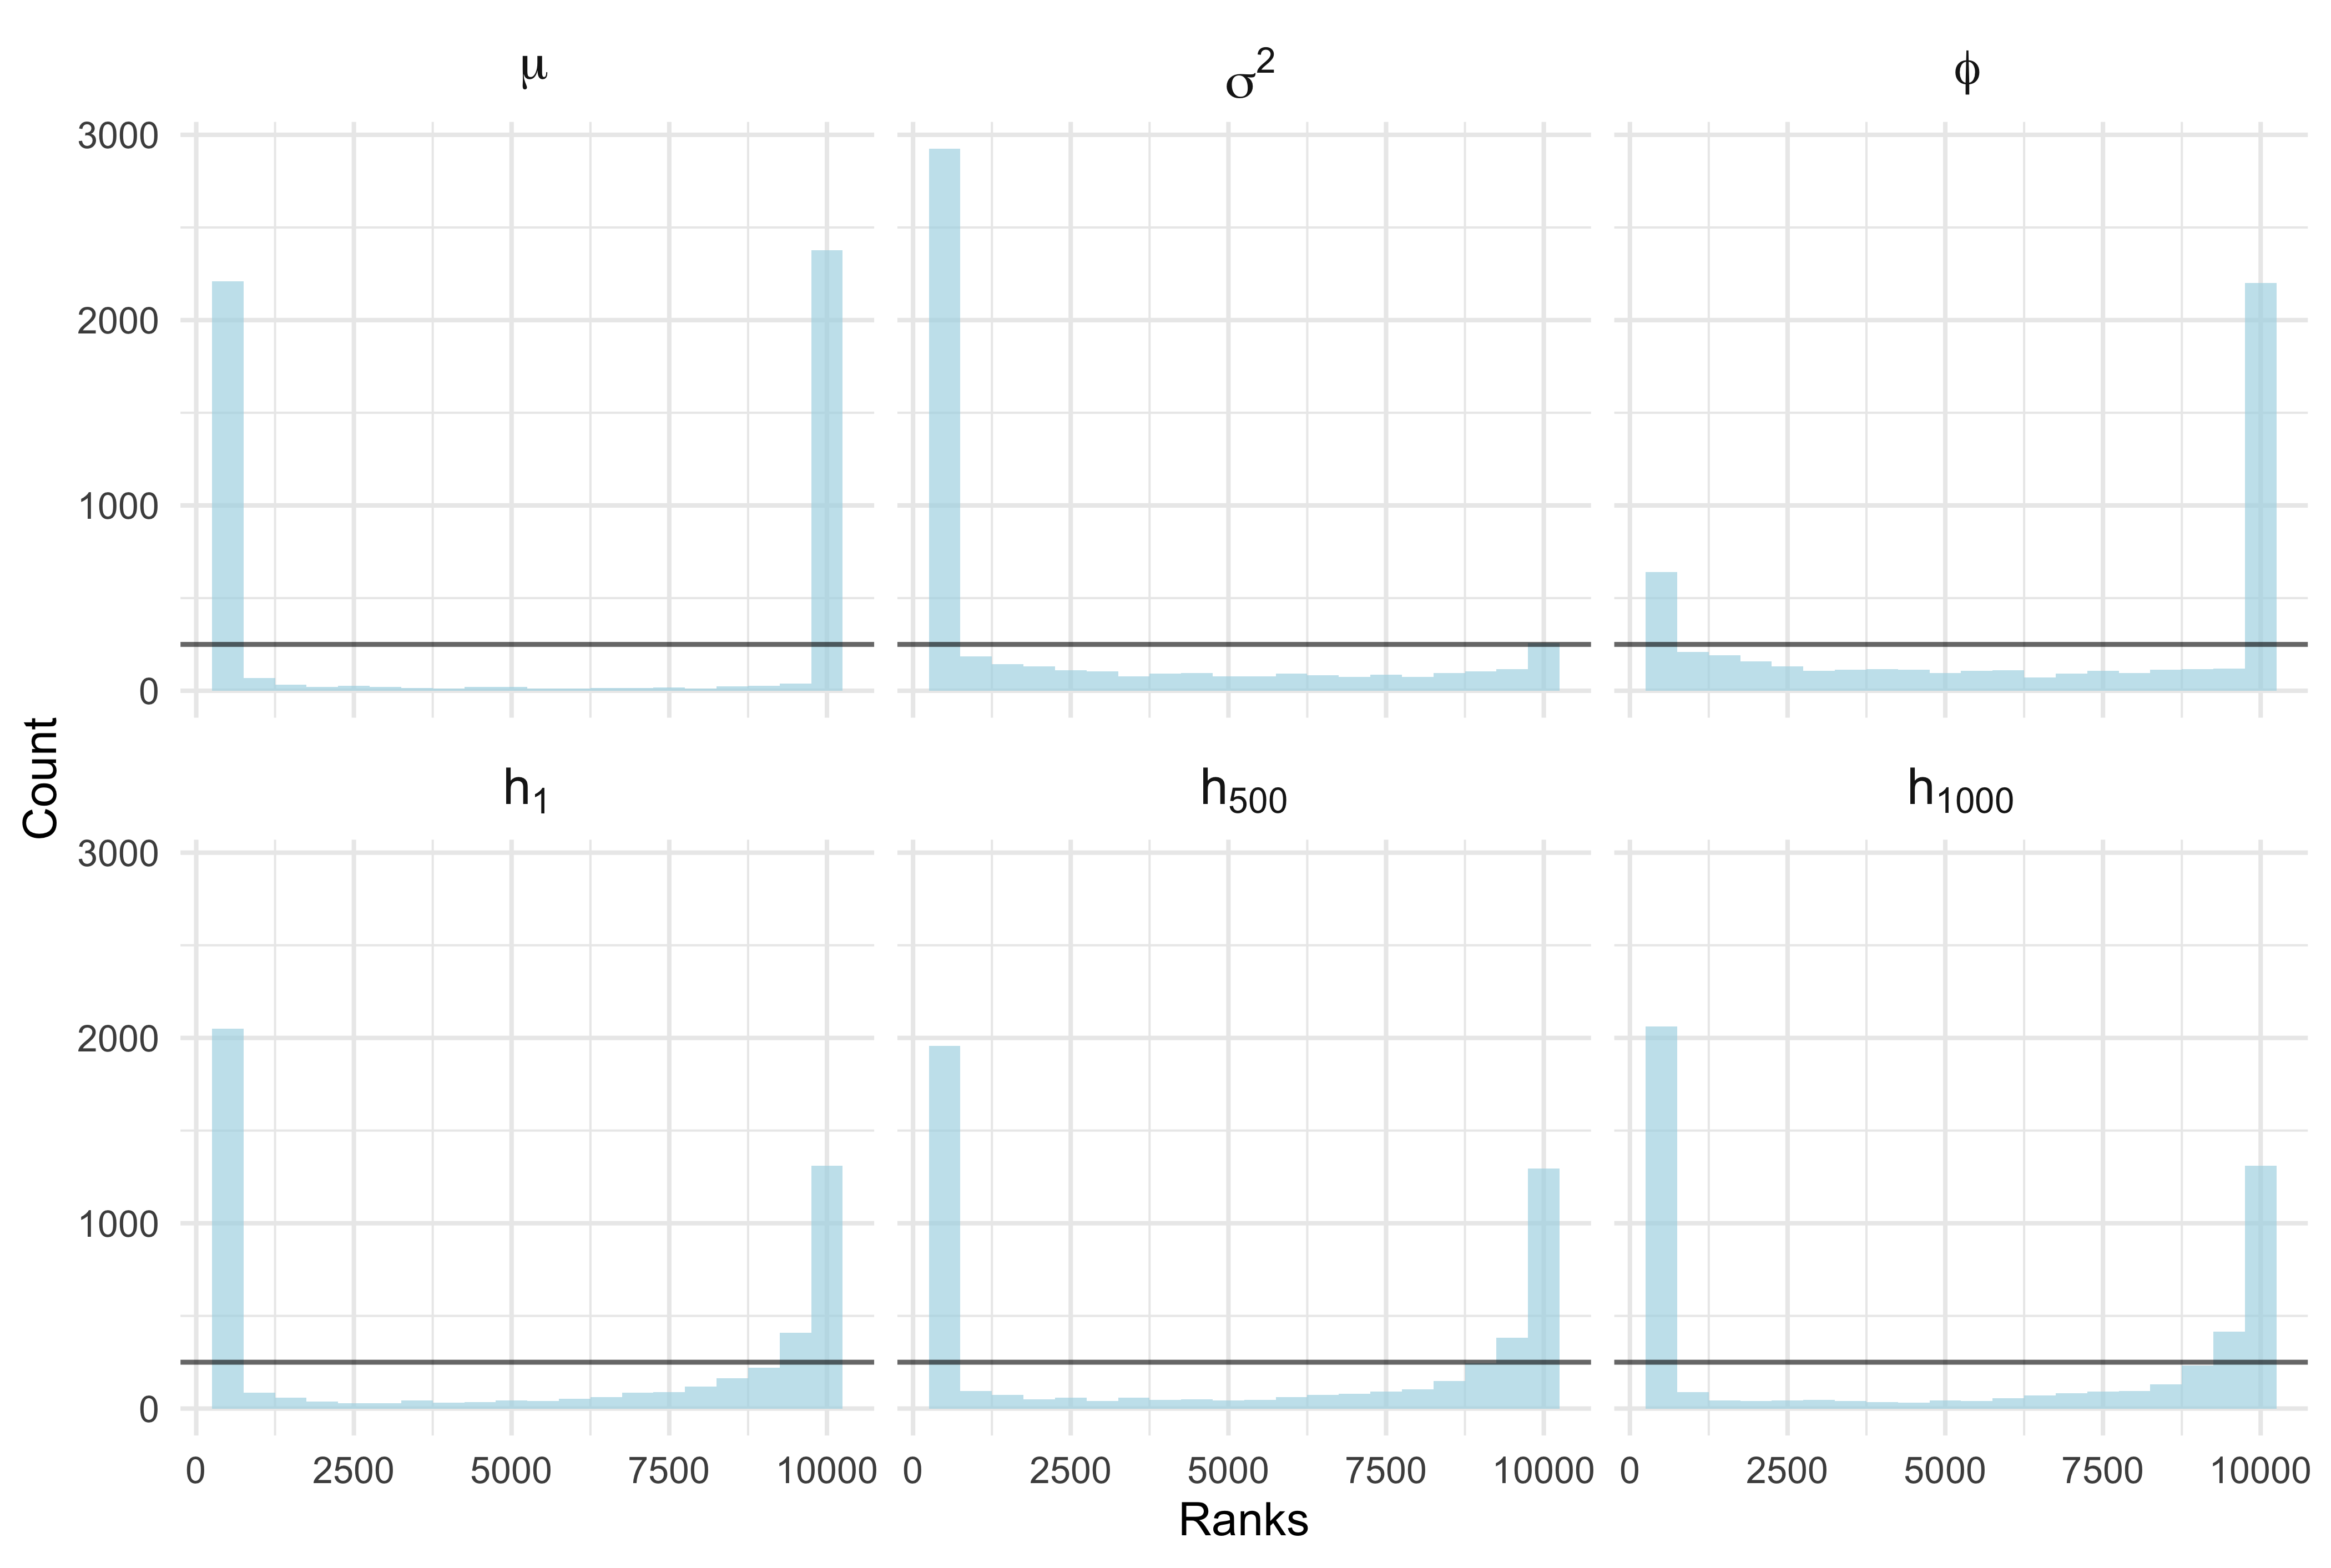
\includegraphics[scale=0.09]{results/ksc_ncp_5k.png}
        \caption{5000 SBC iterations for non centered Gaussian mixture approximation model. No improvement is observed in the distribution of rank statistics. The MCMC returns uncalibrated posterior estimates for this parametersation of the model.}
        \label{fig:ncpksc5k}
    \end{figure}

    The ESS estimates for this model indicate a high degree of autocorrelation and difficulty in generating independent samples from both parameterisations. The numerical results are summarised in Figure \ref{fig:kscess} and Table \ref{tab:kscess}. The estimate for $\mu$ in the reparameterised model exhibits a long right tail (longer than the 10,000 posterior draws suggesting the presence of negatively autocorrelated draws). There is some improvement in efficiency from the reparameterised model with higher ESS values across most of the static parameter quantiles. Overall, the KSC bespoke MCMC is inefficient at sampling the static parameters. 
    
    % The median ESS for $\mu$, $\phi$ and $\sigma^2$ are 559, 103, 39.5 respectively for 10,000 post burn in draws. Despite having 10 times the number of draws, the number of effectively independent samples is much smaller relative to HMC, suggesting that this bespoke sampling strategy is highly inefficient. 

    % - reparam has massive long tail for mu

    \begin{figure}[H]
        \centering
        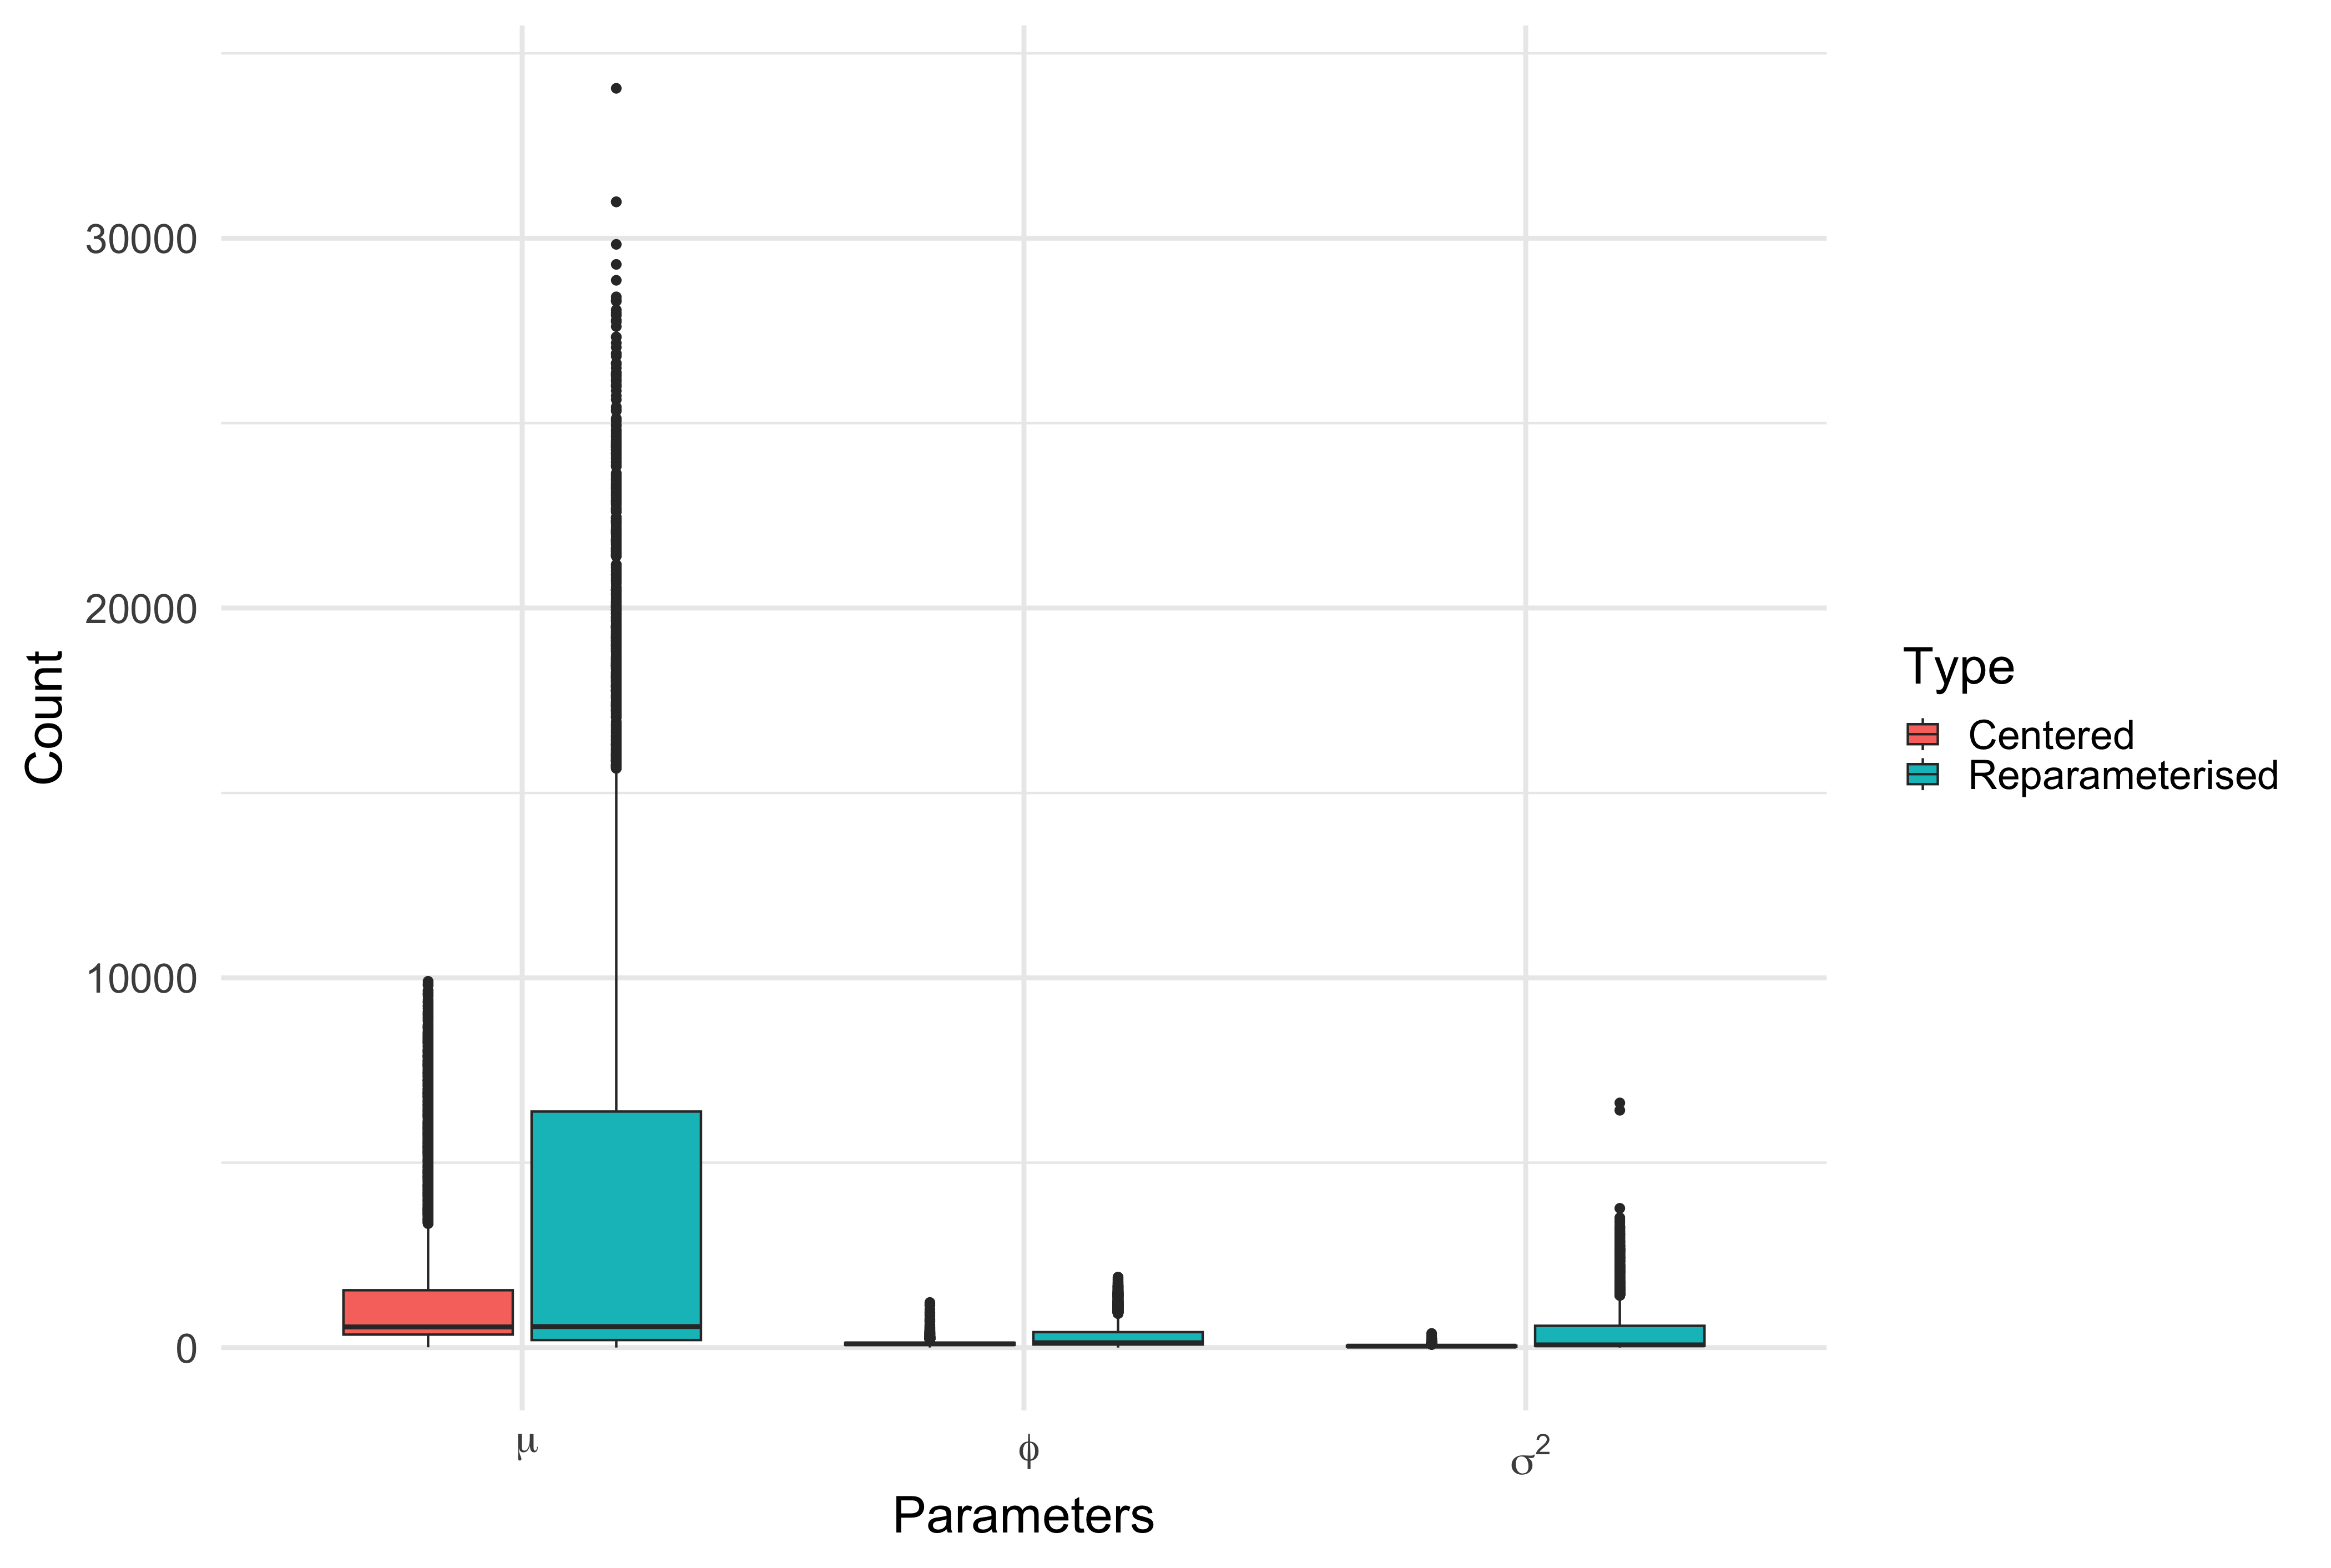
\includegraphics[scale=0.1]{results/ksc_ess.png}
        \caption{Effective sample sizes for static parameters after 5000 iterations of SBC and 1000 post burnin samples for the Gaussian Mixture model. The bespoke sampling strategy struggles to generate independent samples for all static parameters, suggesting a high degree of autocorrelation in the Markkov Chain.}
        \label{fig:kscess}
    \end{figure}

    \begin{table}[H]
        \centering
        \begin{tabular}{|c|c|c|c|c|c|c|c|} \hline 
        Parameter &  Type&Min& q25&  Median& Mean & q75&Max\\ \hline 
        $\mu$&  Centered&9.57 & 352. & 559. & 1482. & 1552. & 9907.\\
     $\mu$&  Reparam&1.99 & 205. & 569. & 4174. & 6384. & 34055.\\\hline 
     $\phi$&  Centered&2.47 & 74.0 & 103. & 112. & 130. & 1222.\\
     $\phi$&  Reparam&1.03 & 83.4 & 132. & 325. & 419. & 1907. \\ \hline 
     $\sigma^2$&  Centered&2.33 & 29.0 & 39.5 & 44.2 & 52.8 & 384. \\ 
     $\sigma^2$&  Reparam&1.25 & 47.4 & 73.4 & 399. & 591. & 6618. \\ \hline
        \end{tabular}
        \caption{KSC: ESS for centered and reparameterised stochastic volatility model.}
        \label{tab:kscess}
    \end{table}

    The results from the KSC algorithm indicates issues with calibration. The centered parameterastion appears to be more favourable for this sampling approach. Other ways of improving the sampling of this model using this MCMC strategy could be to use another parameterisation such as non centered in scale.

    There are a few potential reasons for the poor calibration results. It may be due to the ineffectiveness of the MCMC strategy to generate the correct posteriors. Additionally, it could be due to the approximation of the actual stochastic volatility model not producing accurate posterior estimates. Correcting potential approximation error of the model is explored in the next section.  

    \subsection{Correcting approximation error using importance weights}
    \citet{kim1998stochastic} correct for approximation error in their method by using importance weights. The reweighting procedure ensures that samples are drawn from the correct posterior density. This is applied to the calculation of the expected value of the stochastic volatility posterior density using samples drawn from the Gaussian mixture model. 

    Importance weights are defined as the ratio of the joint posterior from the stochastic volatility model and the posterior distribution of the approximate model. A weight is produced for each posterior sample generated by MCMC. These weights correct the samples from the approximate distribution by increasing or decreasing the contribution of that sample in the calculation of the expectation. 

    These weights can be applied in an additional sampling step using Metropolis Hastings or Importance Resampling (also known as sampling-importance resampling or SIR) to produce samples from the target posterior. However, the rank statistic can also be written as a function of the weighted expectation of the indicator random variable. This reweighting step is applied to the calculation of the rank statistics to see if the correction improves the calibration of the MCMC sampler.\footnote{Efficiency estimates of the reweighted posterior samples are omitted. It was unclear at the time of writing whether the ESS could be written as a function of the expectation or whether the ESS from resampled posterior samples using the importance weights are valid.}

    \subsubsection{Reweigthing rank statistics of the Gaussian Mixture Model}
    Let $v(\theta, h)$ be the log weights defined as the log difference between the posterior densities of the true model with log chi squared errors $log\: g(\theta, h | y^{\ast}_t)$ and the Gaussian mixture model $log\:  k(\theta, h_t | y^{\ast}_t)$.

    $$
    \begin{aligned}
        v(\theta, h) = log\: g(\theta, h | y^{\ast}_t) - log\:  k(\theta, h_t | y^{\ast}_t) = const + log\: g(y|h) - log\: k(y^{\ast} | h)
    \end{aligned}
    $$

    Take the exponential and normalise the weights for the $l^{th}$ posterior draw (note the constants cancel out):
    
    $$
    \begin{aligned}
    w^l = \frac{exp(v(\theta, h)_l)}{\sum_i exp(v(\theta, h)_i)}
    \end{aligned}
    $$

    This gives the normalised importance weight. The expectation for any function of the posterior samples can be written as a function of these weights. Let $S(\theta)$ be an indicator random variable that is a function of the posterior samples. The expectation can be written as:

    $$
    \begin{aligned}
    S(\theta) &= 1[\theta_l < \theta^{sim}] \\
    E[S(\theta) | y] &= \int s(\theta) g(\theta | y) d\theta\\ 
    &= \frac{\int s(\theta)\times exp(v(\theta, h)) * k(\theta, h_t | y^{\ast}_t)d\theta d h}{\int exp(v(\theta, h)) * k(\theta, h_t | y^{\ast}_t)d\theta d h} 
    \end{aligned}
    $$

    Therefore, the expectation of the reweighted posterior samples is given by:

    $$
    \begin{aligned}
    E[S(\hat{\theta}) | y^{\ast}] = \sum_l^L S(\hat{\theta}_l)w_l
    \end{aligned}
    $$

    The rank statistic can be rewritten as a function of the expectation and weights. This gives us the reweighted rank statistics.

    $$
    \begin{aligned}
    r = \sum_{l=1}^{L}1[\theta_{l} < \theta^{sim}] \approx  L\times E[S(\hat{\theta})] = L\times \sum_l^L S(\hat{\theta}_l)w_l
    \end{aligned}
    $$

    The results from applying this reweighting step to the rank statistics of the centered model are given on Figure \ref{fig:reweight1k}. There are no improvements in the distribution of rank statistics. Increasing the SBC iterations to 5000 as seen in Figure \ref{fig:reweight5k} also show no major improvements. The shape of both sets of histograms is consistent with the shape of the unweighted rank statistics. Overall the reweighting of the posterior samples from the approximate model does not improve the calibration results. The reweighted rank statistics for the reparameterised model also did not improve and can be found in Appendix D.

    \begin{figure}[H]
        \centering
        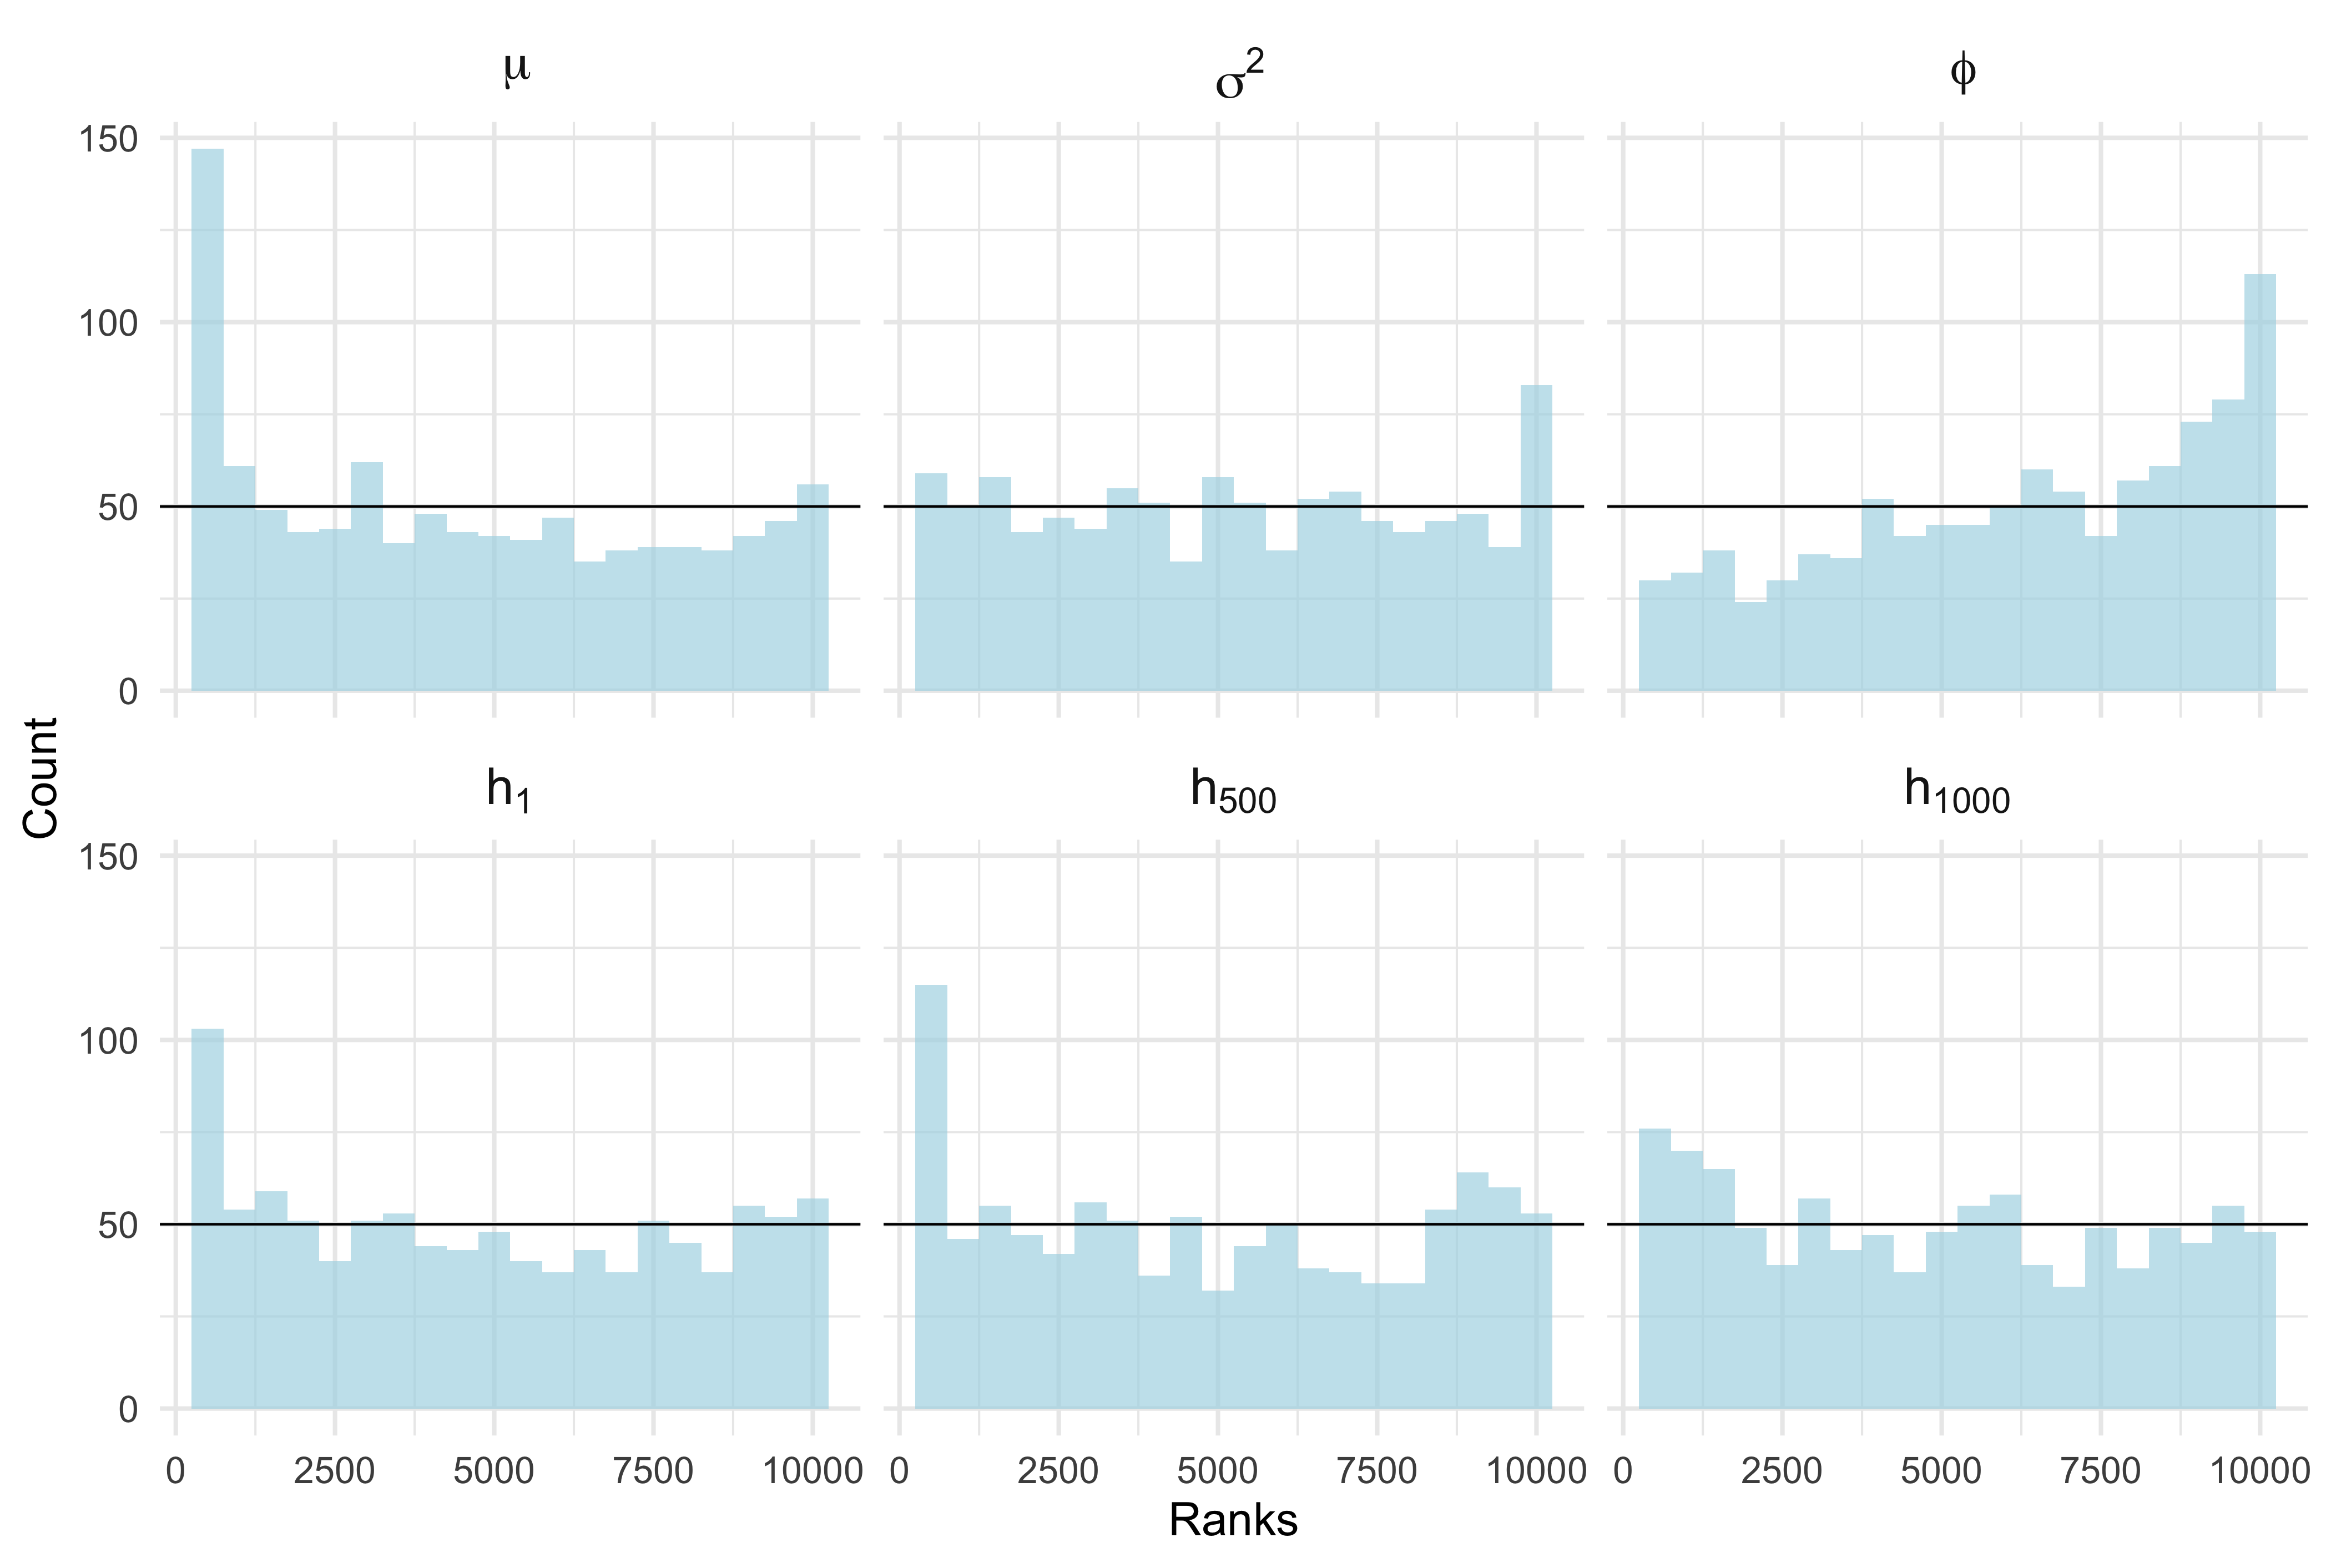
\includegraphics[scale=0.1]{results/weighted_ksc_cp_1k.png}
        \caption{1000 SBC iterations for reweighted rank statistics from the Gaussian mixture approximation model. The shape of the histogram is consistent with the unweighted rank statistics.}
        \label{fig:reweight1k}
    \end{figure}

    \begin{figure}[H]
        \centering
        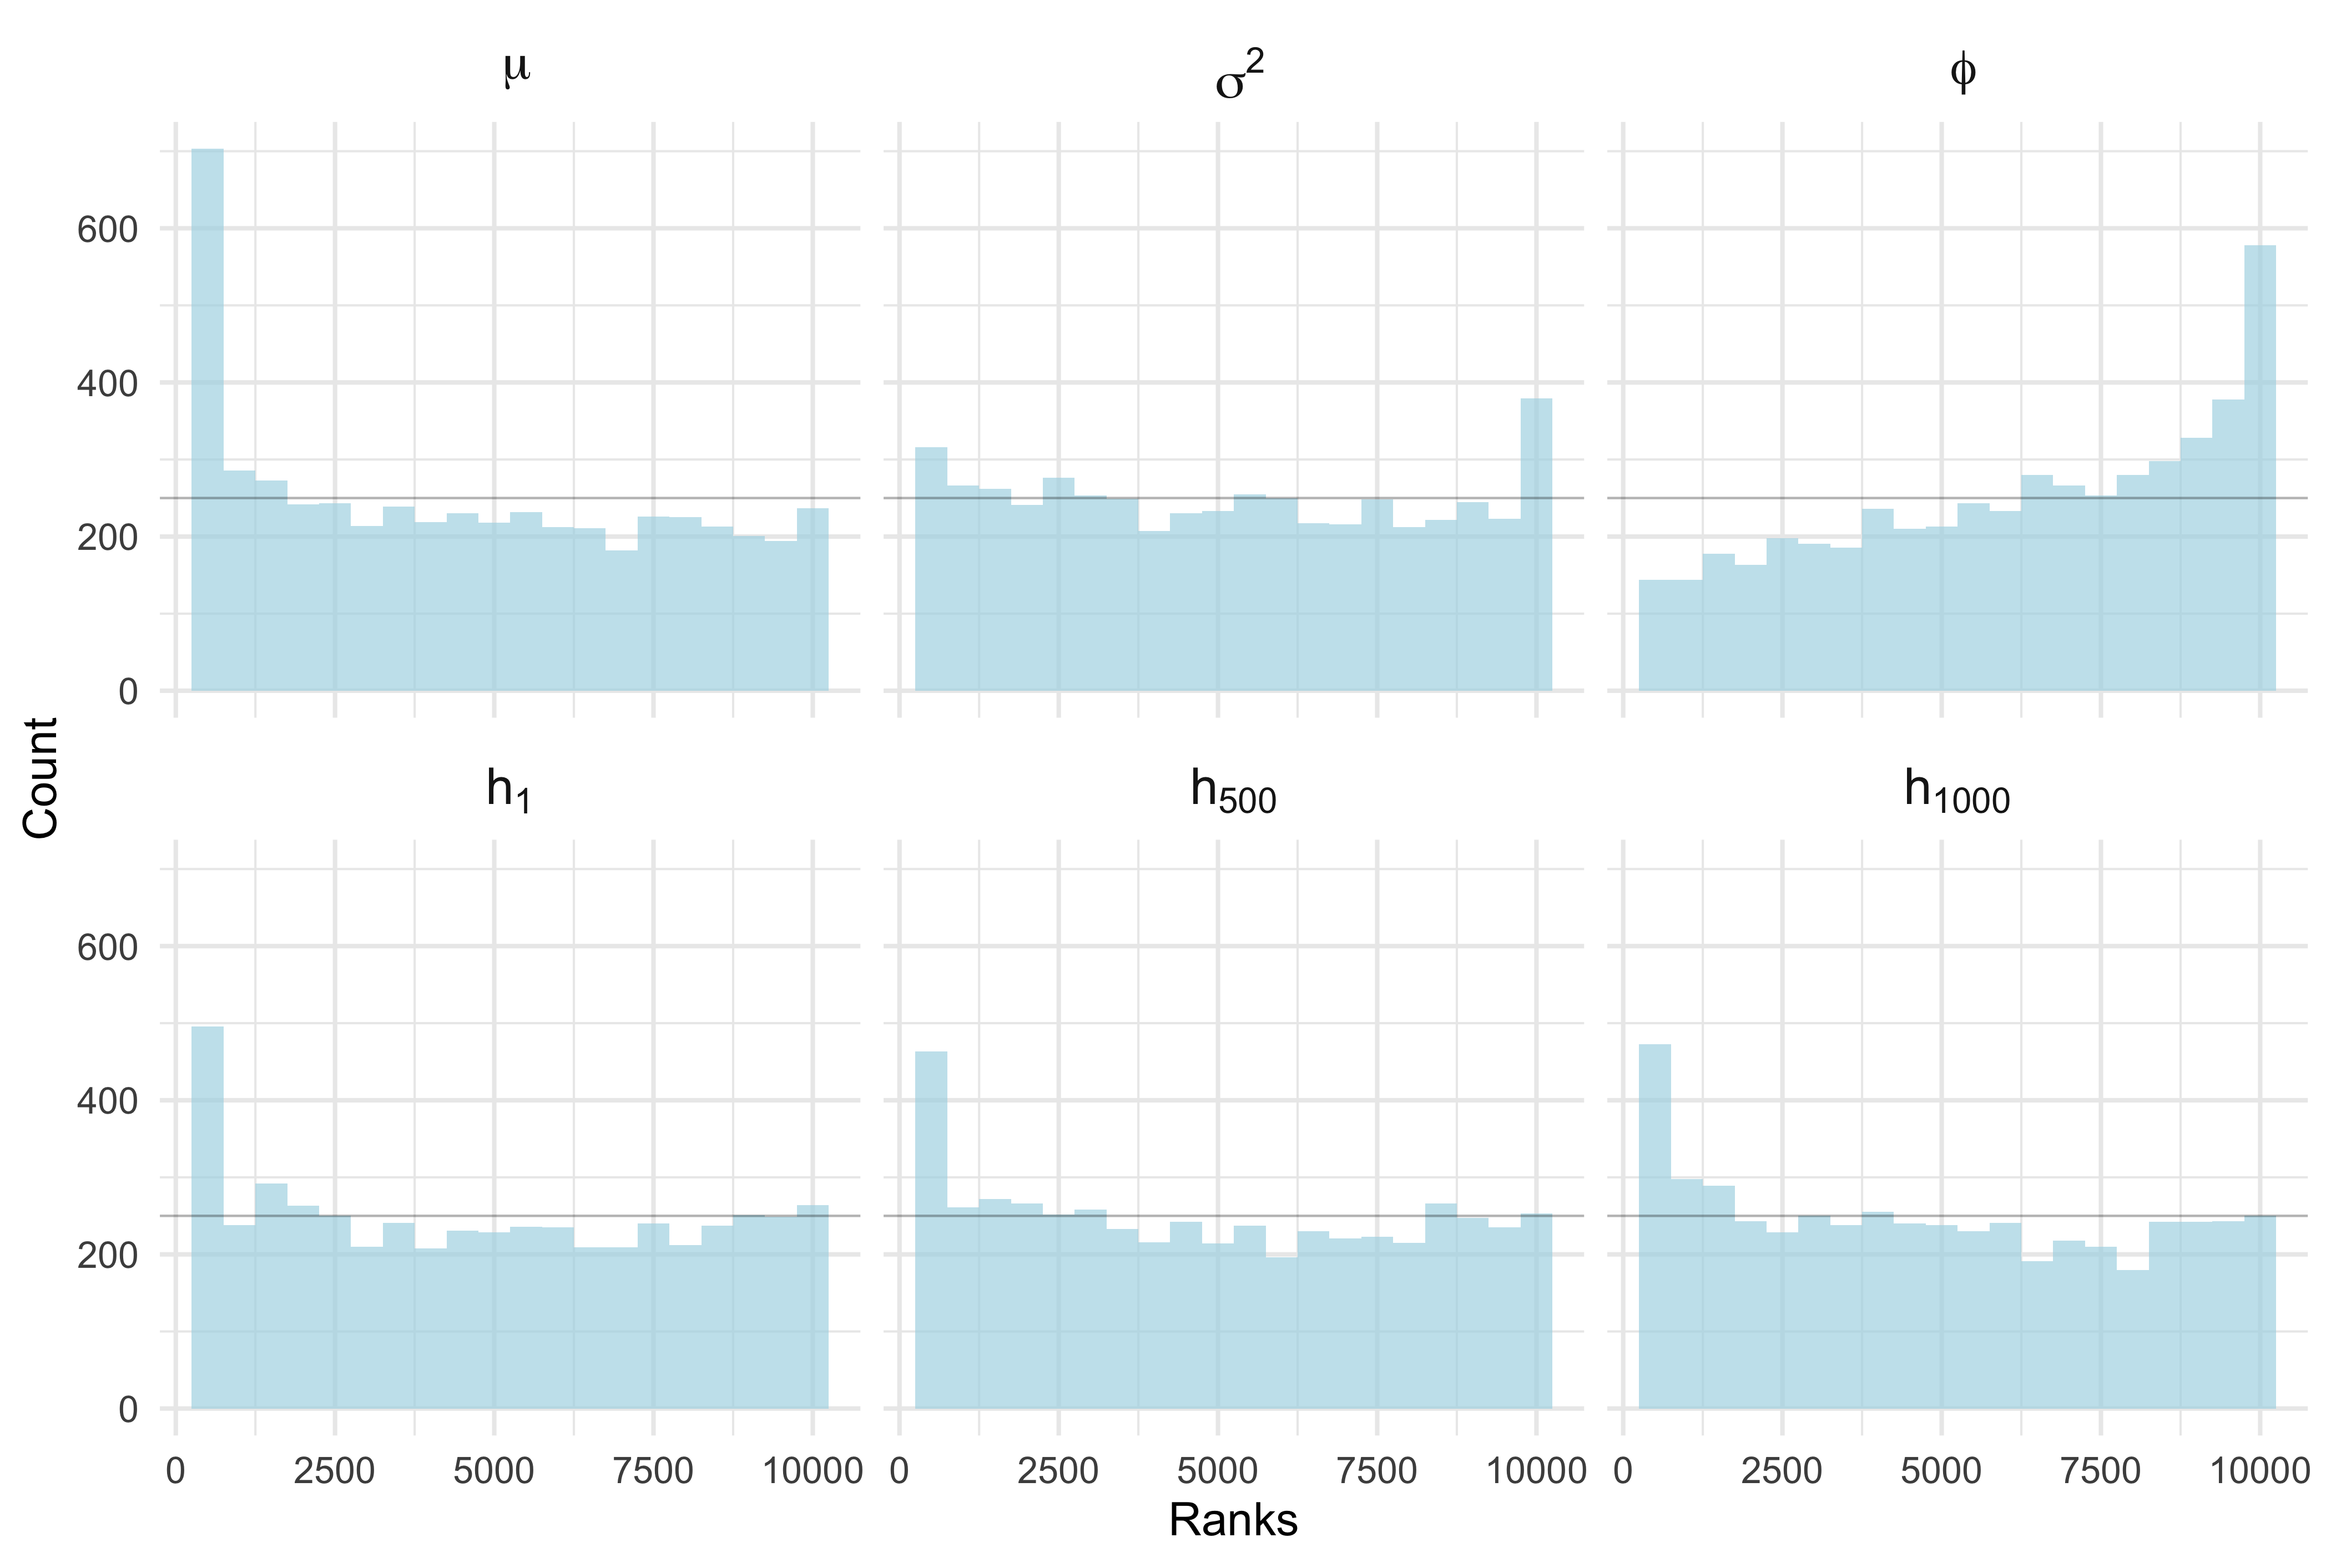
\includegraphics[scale=0.1]{results/weighted_ksc_cp_5k.png}
        \caption{5000 SBC iterations for reweighted rank statistics from the Gaussian mixture approximation model. No major improvements are observed to the uniformity of rank statistics.}
        \label{fig:reweight5k}
    \end{figure}

    \subsection{Evaluating SBC for state parameters}
    As discussed, it is not practical to inspect the histograms of all parameters and states in the stochastic volatility model. Instead, the chi squared statistic can is used to summarise the shape of the rank statistic distribution. This will be used to summarise the state variables only since the static parameters can be compared across simulations individually. 

    The state variable chi squared statistics for centered and reparamterised HMC, centered KSC and centered importance weighted KSC are reported as histograms in Figure \ref{fig:allchisq} (using results from 5000 SBC iterations). Reparameterised KSC is omitted as its poor SBC performance just adds noise to the results. A chi squared statistic of 0 implies the sample is exactly uniformly distributed. Any value away from 0 captures variation or deviations from uniformity. This provides a high level summary of the state variables - how close their rank statistics are to being uniformly distributed and their distance relative to the other algorithms and parameterisations. 
    
    The HMC results are relatively close to zero. Both KSC and the importance weighted ranks on the other hand are far from zero suggesting major deviations from uniformity. There is a large gap between the HMC and KSC chi squared statistics implying the distribution of state variable ranks are much less uniform for KSC relative to the HMC. Combined with the results in the previous section, there is a strong evidence that HMC outperforms KSC where it comes to calibration across all parmeters and latent state variables.

    \begin{figure}[H]
        \centering
        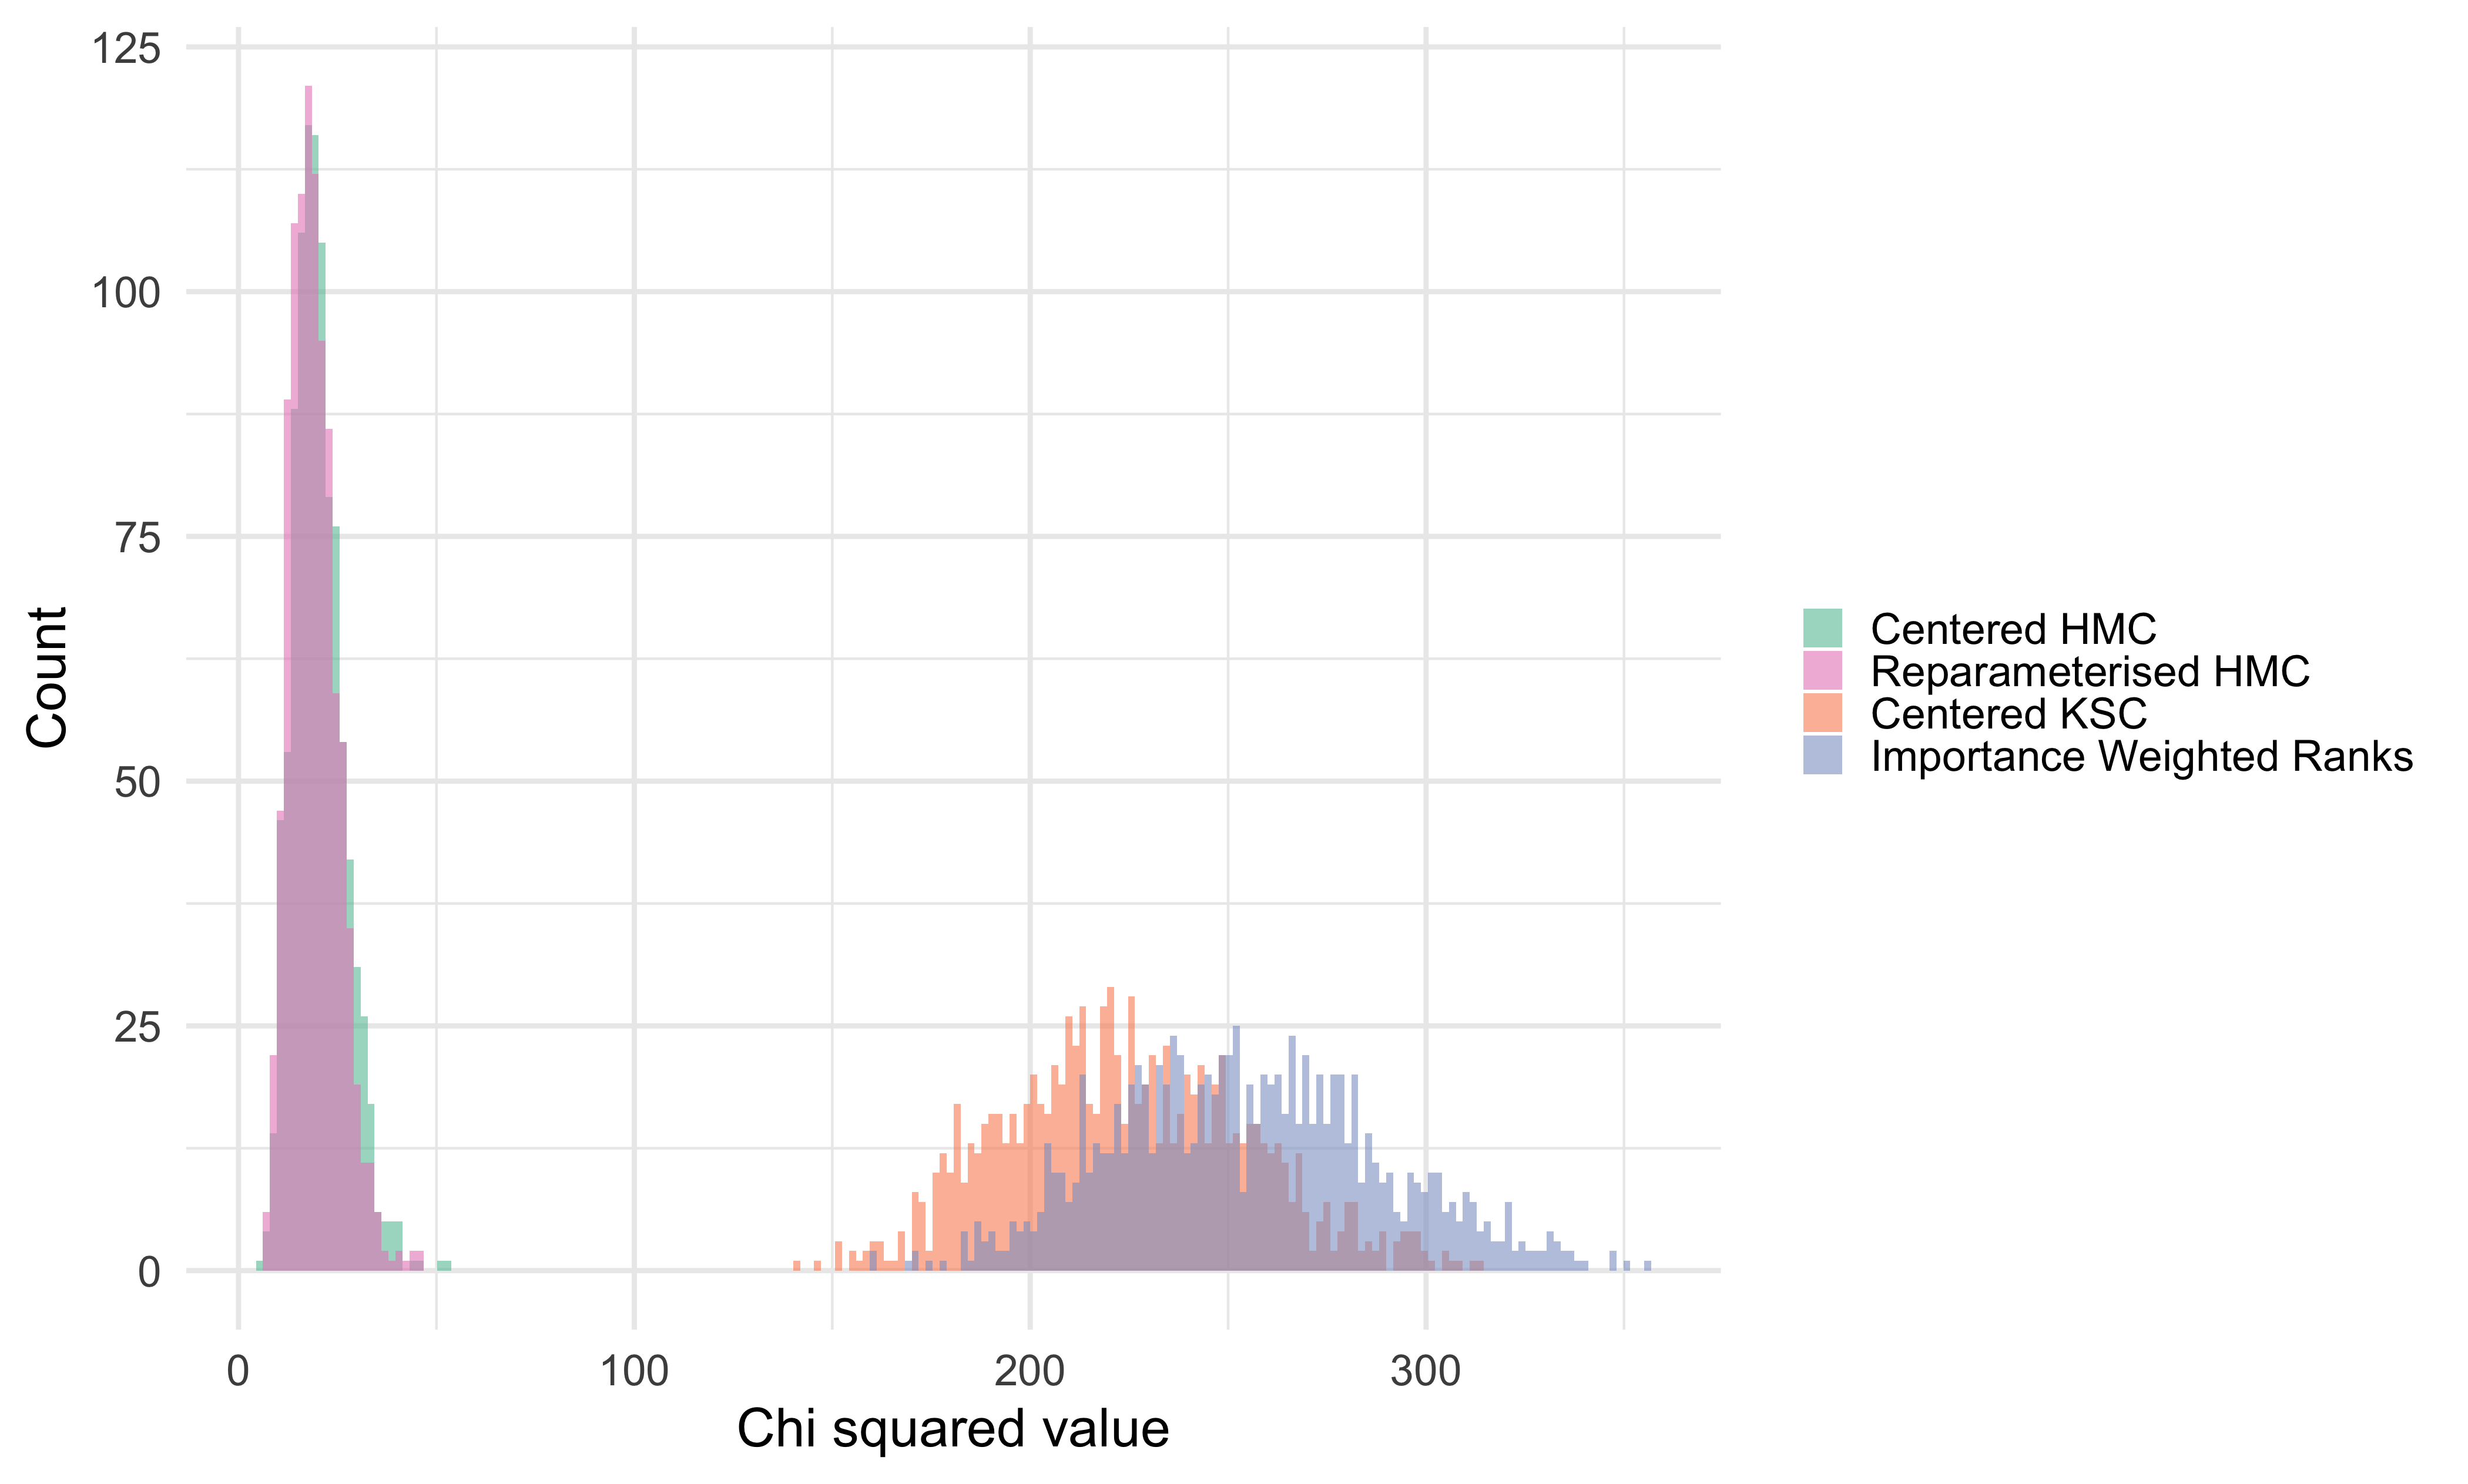
\includegraphics[scale=0.1]{results/dist_chisq_all.png}
        \caption{Distribution of chi squared statistics for latent state variables. Results from 5000 SBC iterations are used. Values closer to 0 are more consistent with a discrete uniform distribution. Both HMC simulations are much closer to zero than KSC. This suggests that the HMC algorithm overall produces more calibrated posterior estimates for the state variables}
        \label{fig:allchisq}
    \end{figure}

\section{Discussion}
Overall, Hamiltonian Monte Carlo applied on the reparameterised model performs best based on calibration and efficiency results. Centered parameterisation using HMC performed moderately well but struggled to produce calibrated posterior estimates for $\sigma^2$ and $\phi$ as well as generate independent samples for these parameters. Gaussian mixture approximation struggled to return calibrated posterior estimates and efficient samples for both parameteristions. However, the centered parameteristion results for the Gaussian mixture model may improve if we increased the length of the Markov chain. This is discussed later in the limitations section. 

These results demonstrate that the performance of a MCMC algorithm is sensitive to the paramterisation of the model in the context of calibration and efficiency. Furthermore, the paramterisation of a model is conditional on the choice of MCMC algorithm. Evaluating the effectiveness of a modelling strategy (i.e choice of model, paramterisation and sampler) on simulated data gives a lot of a priori information about how the model will perform before it is fit on real data. Performing SBC may help isolate confounding factors if any problems occur. 

The priors chosen for this study came directly from \citet{kim1998stochastic}. The SBC results for the Gaussian mixture may improve if the priors were more informative - although this is only conjecture. Whether or not to use tighter priors depends on the modelling context and the problem at hand. If a model is expected to handle data generated by the priors, then uncalibrated results from SBC raises questions about the suitability about the model choice, MCMC or parameterisation. 

Other parameterisaions of the stochastic volatility model are available as outlined in \citet{strickland2008parameterisation}, namely non centered in scale or both non centered in scale and location. The failure of non centered parameterisaion in location for the Gaussian mixture model could be due to a variety of reasons. This may be due to a particular software implementation when it comes to the Kalman Filter and Simulation Smoother (where a specific software package was applied) that was not designed to handle the non centered parameterisations. Or perhaps this particular parameterisation does not suit the sampling strategy applied by KSC and another approach (e.g. HMC) might be more successful. Lots of different design and implementation details could be explored further. Pinpointing the reason why this model parameterisation failed as well as exploring other configurations and MCMC algorithms in this context is left to future research.

It is worth noting that there are many ways of comparing MCMC approaches. Other features that may be of interest is the speed in which a MCMC can converge onto the target distribution and generate samples for inference. However, speed is diffiuclt to define and is subject to a variety of different factors such as hardware, operating system, and software versions. The purpose of this research is to compare algorithms based on calibration and efficiency. Additionally, this simulation study does not provide any advice on the appropriateness of the stochastic volatility model on real data. Whether the stochastic volatility model is appropriate for modelling a particular financial time series requires further study into the data generating process, domain expertise and a suite of other diagnostic checks. Examples of this are posterior predictive checking and out of sample predictive performance. Rather, the SBC approach gives insight into how well calibrated a sampling strategy is conditional on a known data generating process which is important in all applied contexts.  

% (other implementations exist as well but left for future research. lots of different design and implementation details could be explored. Let alone choice of algos.)

\section{Limitations}
A limitation to applying SBC in all modelling contexts is that it is computationally intensive. SBC requires fitting multiple models to get reliable estimates. In some cases, fitting just one model can take a long time, let alone multiple. Producing results for this research within a reasonable timeframe required use of a computer cluster. Computing infrastructure may limit the opportunity for SBC to be performed, although it is probably not necessary to do 5000 SBC iterations in other research contexts. The choice of SBC iterations for this research was arbitrary and was used to demonstrate that noisy estimates could be reduced by increasing the number of iterations for calibrated models. A more principled approach to picking the number of SBC iterations could be explored in other research.

Diagnostic tools for evaluating SBC results and models with many parameters is an area for improvement. As discussed, inspecting many histograms for highly parameterised models is unrealistic. Other summary statistics and visualisations can be applied for a high level comparison, such as the chi squared statistics applied in this research. Furthermore, it is not always straightforward to understand why any any one parameter may produce poor calibration results, for example, an arbitrary state parameter. SBC may tell us some information about the miscalibration based on the histogram shape (e.g. under or over dispersed relative to the prior distribution), but understanding why this occurs may not be immediately clear. Although, diagnosing sampling problems with complicated posterior geometries speaks more generally to the difficulty of understanding complex models in the first place as opposed to a limitation of SBC.

Lastly, it is unclear what constitutes a fair comparison between algorithms when comparing SBC results. In particular, the number of post burnin or warmup samples differed between algorithms (999 post burn-in for HMC, 9999 for the bespoke algorithm). An argument could be made that the poor results for the bespoke KSC algorithm may be due to the chain not converging onto the target distribution. Indeed, the authors of this approach extended their Markov chain to 750,000 posterior draws. A farier comparison may be to have roughly similar number of ESS for most of the estimated parameters, although this is difficult to get right with a large number of parameters and variables to estimate. Given how well Hamiltoninan Monte Carlo performed with the reparamterised model, any improvement to the Gaussian mixture model by increasing the length of the Markov chain would make calibration just as good, but not better due to the inefficiency of the sampler. 

\section{Conclusion}
This research evaluated and compared different MCMC algorithms for fitting stochastic volatility models. As our models and algorithms for estimating these models become more complicated, so does the need for principled ways of checking that they are returning correct posterior estimates. SBC provides a general simulation design to check whether a modelling strategy is producing calibrated results for generative models.

In the context of stochastic volatility, applying Hamiltonian Monte Carlo on a reparameterised stochastic volatility model provided the most calibrated and efficient estimates when compared with KSC's bespoke MCMC method. This also outperformed the KSC model using importance sampling weights to correct for approximation error. Other parameterisations of the stochastic volatility model can be considered to see if it improves sampling performance based on these diagnostics. 

This study only considered a handful of potential algorithms, sampling strategies and parameterisations for stochastic volatility. Future research could use the same SBC design to compare and evaluate more complicated volatility models and MCMC algorithms. Overall, SBC is a valuable tool in model development and is a key part of a statistical workflow. 
 
\newpage

\bibliography{references}

\newpage

\section{Appendix A: Mixture Gaussian weights}

\begin{table}[H]
    \centering
    \begin{tabular}{lccc} 
          $\omega$ &$Pr(\omega = i)$&  $m_i$&  $\nu^2_i$\\ 
          1&0.00730  &  -10.12999&  5.79596\\ 
          2&0.10556  &   -3.97281 &  2.61369\\ 
          3&0.00002 &  -8.56686 &   5.17950\\ 
          4&0.04395 &  2.77786  &   0.16735 \\ 
          5&0.34001&   0.61942    &  0.64009\\ 
          6&0.24566 &  1.79518    &  0.34023 \\ 
          7&0.25750 &  -1.08819    &  1.26261\\ 
    \end{tabular} 
\end{table}

\newpage

\section{Appendix B: Sampling from mixture of Gaussians}

\subsection*{Conjugate posterior distributions}

\textbf{Sampling} $\boldsymbol{\sigma_{\eta}^2}$

Inverse gamma conjugate posterior distribution:

$$
\sigma^2_{\eta} | y,h,\phi,\mu \sim IG \Bigl\{\frac{n+\sigma_r}{2}, \frac{0.05 + (h_1 - \mu)^2 (1 - \phi^2) + \sum_{t=1}^{n-1}((h_{t+1} - \mu) - \phi(h_t - \mu))^2}{2}\Bigr\}
$$

\textbf{Sampling}  $\boldsymbol{\mu}$

Gaussian conjugate posterior distribution:

$$
\mu | h,\phi,\sigma^2_{\eta}  \sim N(\hat{\mu}, \sigma^2_{\mu})
$$

Where

$$
\begin{aligned}
\hat{\mu} &= \sigma^2_{\mu} \Bigl\{\frac{(1-\phi^2)}{\sigma_{\eta}^2}h_1 +\frac{(1-\phi^2)}{\sigma_{\eta}^2} \sum_{t=1}^{n-1} (h_{t+1} - \phi h_t)\Bigr\} \\
\sigma^2_{\mu} &= \sigma^2_{\eta} \{(n-1)(1-\phi)^2 + (1-\phi^2)\}^{-1}
\end{aligned}
$$

\subsection*{Metropolis Hastings Step}
\textbf{Sampling}  $\boldsymbol{\phi}$

Metropolis Hastings accept/reject procedure:

1) Generate proposal $\phi^\ast$ from $N(\hat{\phi}, V_{\phi})$ where $\hat{\phi} = \frac{\sum_{t=1}^{n-1} (h_{t+1} - \mu)(h_t - \mu)}{\sum_{t=1}^{n-1} (h_t - \mu)^2}$ and $V_{\phi} = \sigma^2_{\eta} \{\sum_{t=1}^{n-1} (h_t - \mu)^2\}^{-1}$

2) Accept proposal as $\phi^{(i)}$ with probability $e^{\{g(\phi^\ast) - g(\phi^{(i-1)}\}}$ such that $g(\phi) = log (\pi (\phi)) - \frac {(h_t - \mu)^2 (1-\phi^2)}{2 \sigma_{\eta}^2} + \frac{1}{2} log (1-\phi^2)$

\subsection*{Sampling mixture density}

Rewrite mixture density with respect to a indicator variable $s_t$

$$
\begin{aligned}
&z_t | s_t = i \sim N(m_i - 1.2704, \nu^2) \\
&Pr(s_t = i) = q_i
\end{aligned}
$$

Sample $s_t$ from probability mass function: 

$$
\begin{aligned}
Pr(s_t = i | y_t^{\ast}, h_t) \propto q_i f_N(y_t^{\ast} | h_t + m_t - 1.2704, \nu^2)
\end{aligned}
$$

\newpage

\section{Appendix C: Hamiltonian Monte Carlo algorithm description}
Let $\theta$ be a target parameter and $\phi$ be the auxiliary momemtum variable. The Hamiltonian is defined as:

$$
\begin{aligned}
H(\theta, \phi) \equiv - log \: \pi(\theta, \phi)
\end{aligned}
$$

This can be broken down into kinetic energy $K(\theta, \phi)$, the density over the auxiliary momentum, and potential energy $V(\theta)$, the density of the target posterior distribution.

$$
\begin{aligned}
H(\theta, \phi) &= - log \: \pi(\phi | \theta) - log \: \pi(\theta) \\ 
&\equiv  K(\theta, \phi) + V(\theta)
\end{aligned}
$$

 Starting with an initial draw of $\theta$ (user defined or randomly generated), the HMC iteration or proposal is determined by 3 steps.

1) Randomly sample a momentum value

$$
\begin{aligned}
\phi\sim Multinormal(0, M)
\end{aligned}
$$

Where M is some diagnoal mass matrix (assuming independence between momentum variables).

2) Solve the set of Hamiltonian (differential) equations which generates a proposal $(\theta^{\ast}, \phi^{\ast})$

$$
\begin{aligned}
\frac{\partial \theta}{\partial t} &= \frac{\partial H}{\partial \phi} = \frac{\partial K}{\partial \phi} \\
\frac{\partial \phi}{\partial t} &= \frac{\partial H}{\partial \theta} = - \frac{\partial K}{\partial \theta} - \frac{\partial V}        {\partial \theta}
\end{aligned}
$$

Where $\frac{\partial V}{\partial \theta}$ is the gradient of the target posterior density. The solution to these differential equations is approximated using a Leapfrog integrator which gives a discrete approximate solution. The parameters which are tuned in this process are the number of steps $L$ and the size of the steps $\epsilon$. The Leapfrog algorithm performs a half step of $\phi$ and then a full step of the parameter $\theta$, and another half step of the momemtum variable $\phi$ and repeats this $L$ times. The final step is the proposal $(\theta^{\ast}, \phi^{\ast})$.

$$
\begin{aligned}
\phi &\leftarrow \phi - \frac{\epsilon}{2} \frac{\partial V}{\partial \theta} \\
\theta &\leftarrow \theta + \epsilon M^{-1} \phi \\
\phi &\leftarrow \phi - \frac{\epsilon}{2} \frac{\partial V}{\partial \theta}
\end{aligned}
$$

3) Metrpolis Hastings Accept/Reject
Let $(\theta^{t-1}, \phi^{t-1})$ be the values before the Leapfrog integrator.

$$
\begin{aligned}
r = \frac{\pi(\theta^{\ast} | y) \pi(\phi^{\ast})}{\pi(\theta^{t-1} | y) \pi(\phi^{t-1})}
\end{aligned}
$$

With sampled value

$$
\theta^t = \begin{cases}
    \theta^{\ast},& \text{with probability } min(r,1)\\
    \theta^{t-1}, & \text{otherwise}
\end{cases}
$$

\section{Appendix D: Importance weighted rank statistics for reparameterised model}

\begin{figure}[H]
    \centering
    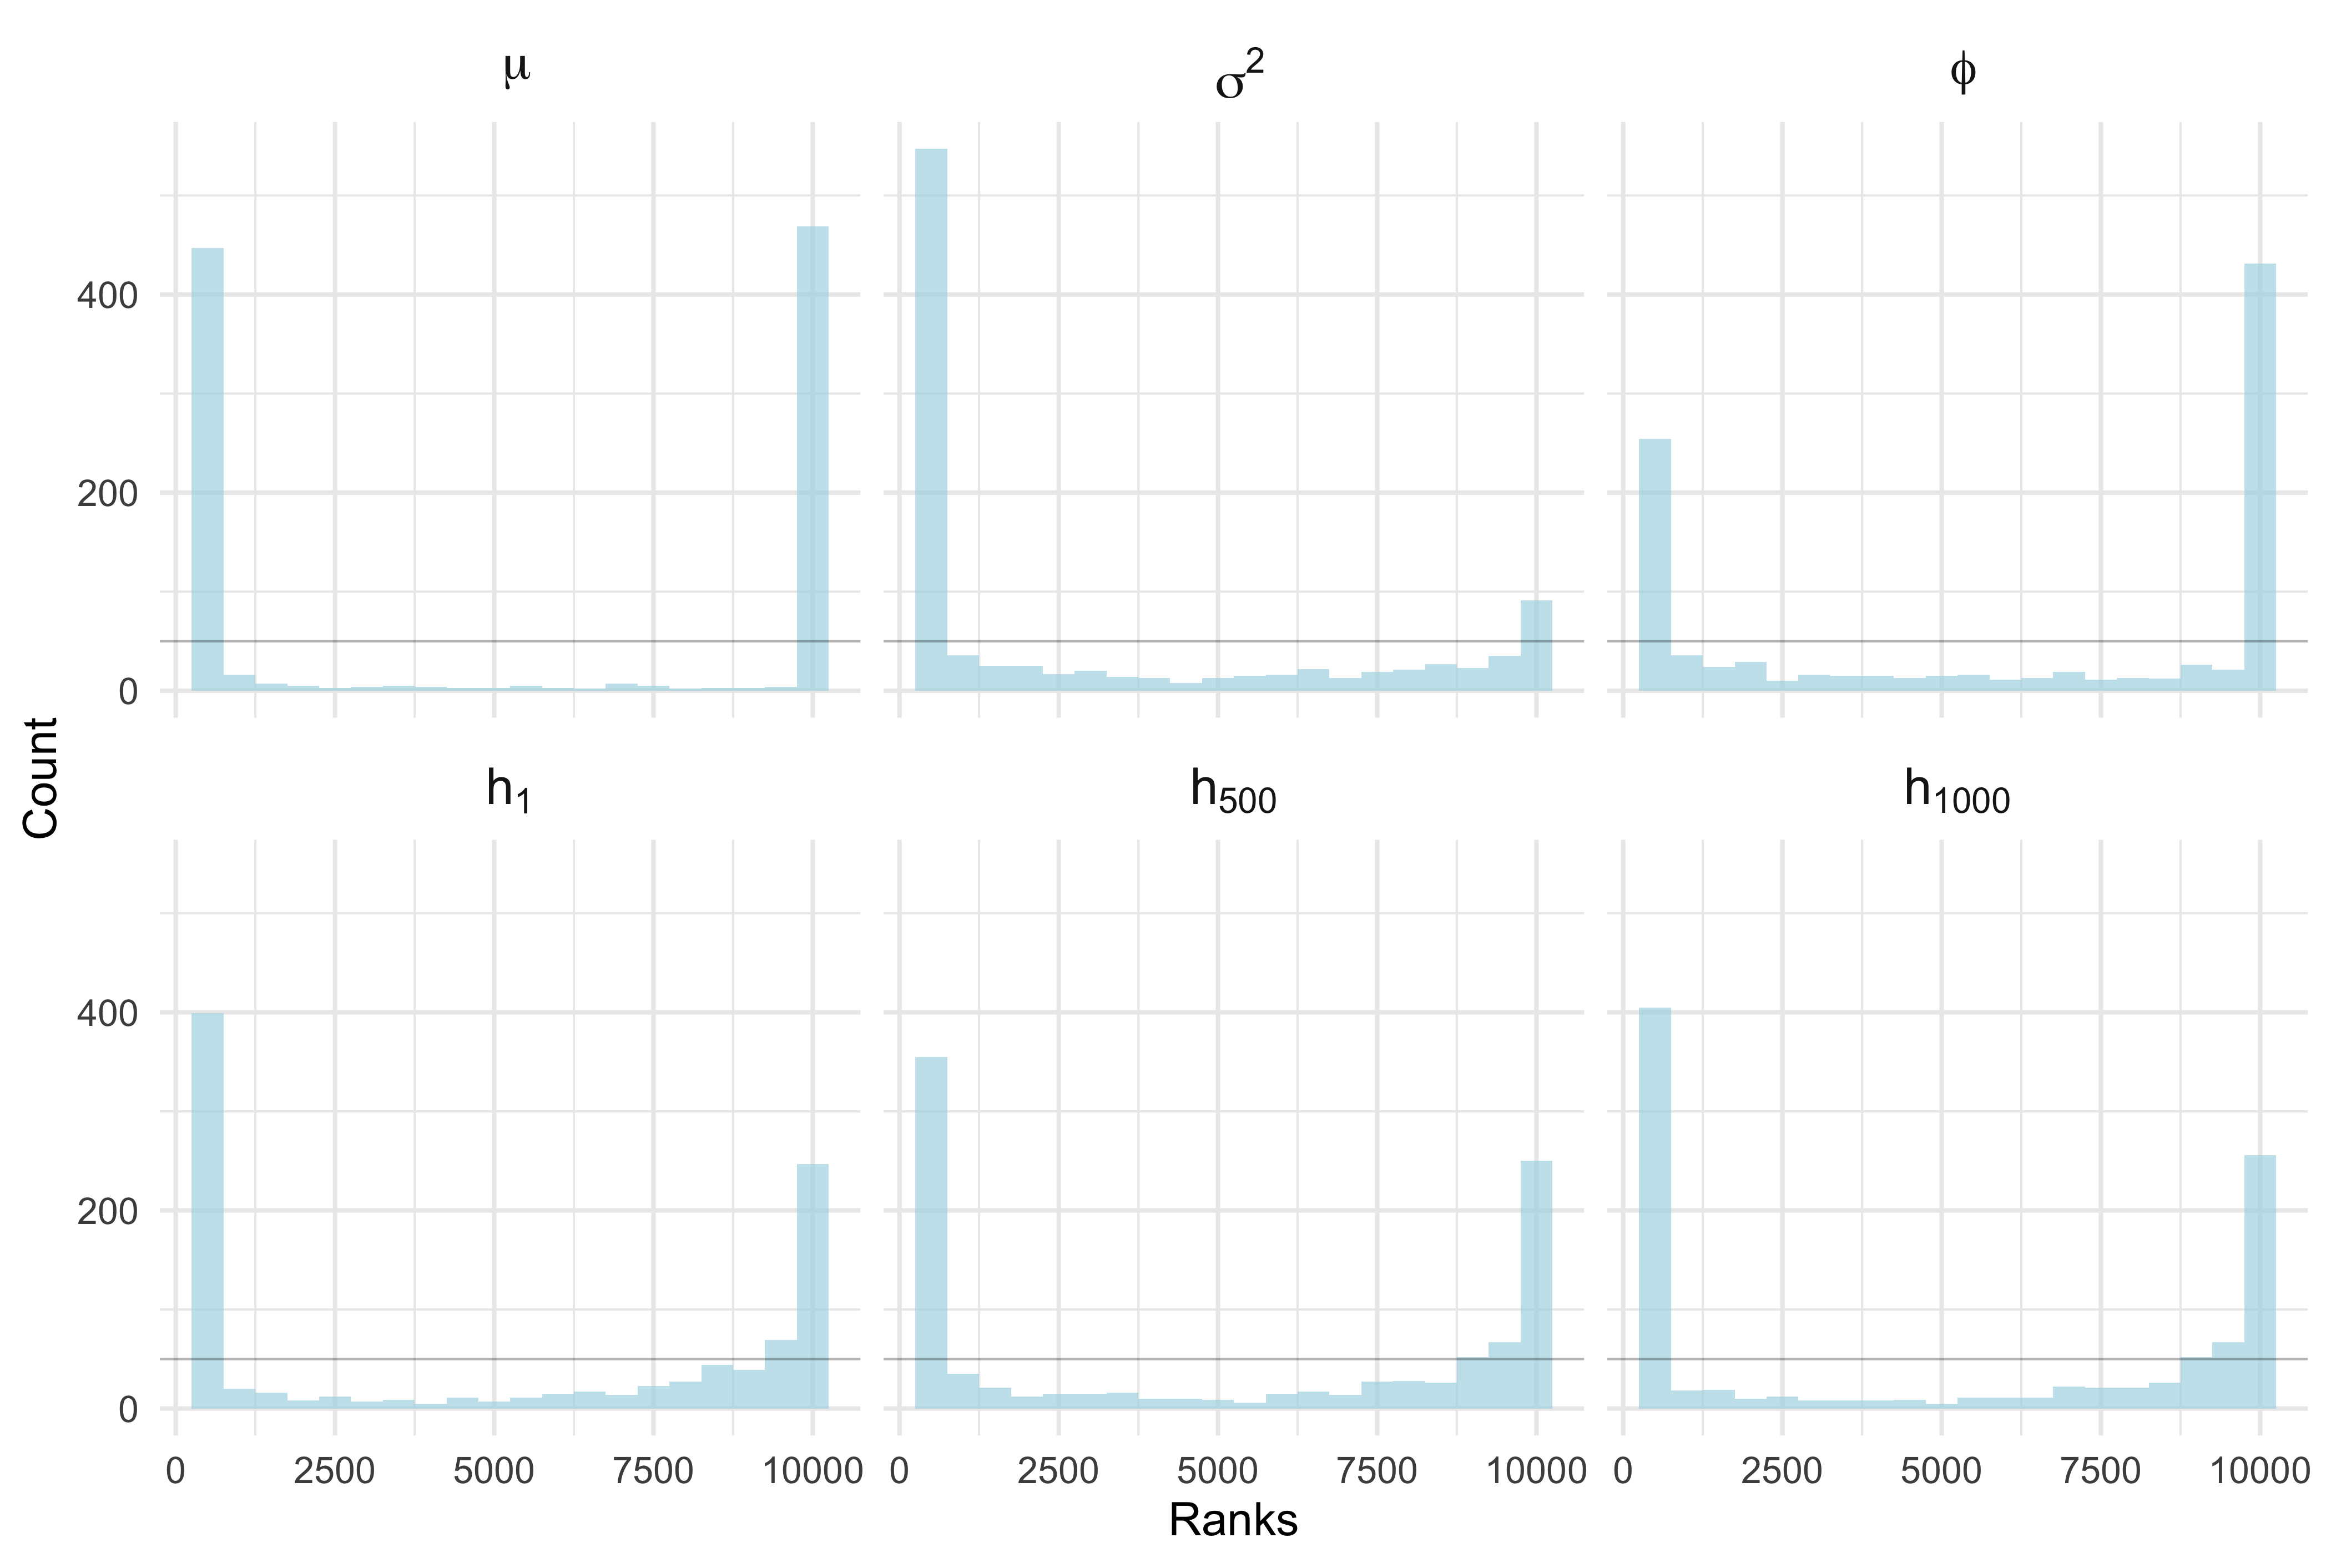
\includegraphics[scale=0.09]{results/weighted_ksc_ncp_1k.png}
    \caption{1000 SBC iterations for reweighted rank statistics from the reparameterised Gaussian mixture approximation model. The shape of the histogram is consistent with the unweighted rank statistics.}
    \label{fig:reweight1k}
\end{figure}

\begin{figure}[H]
    \centering
    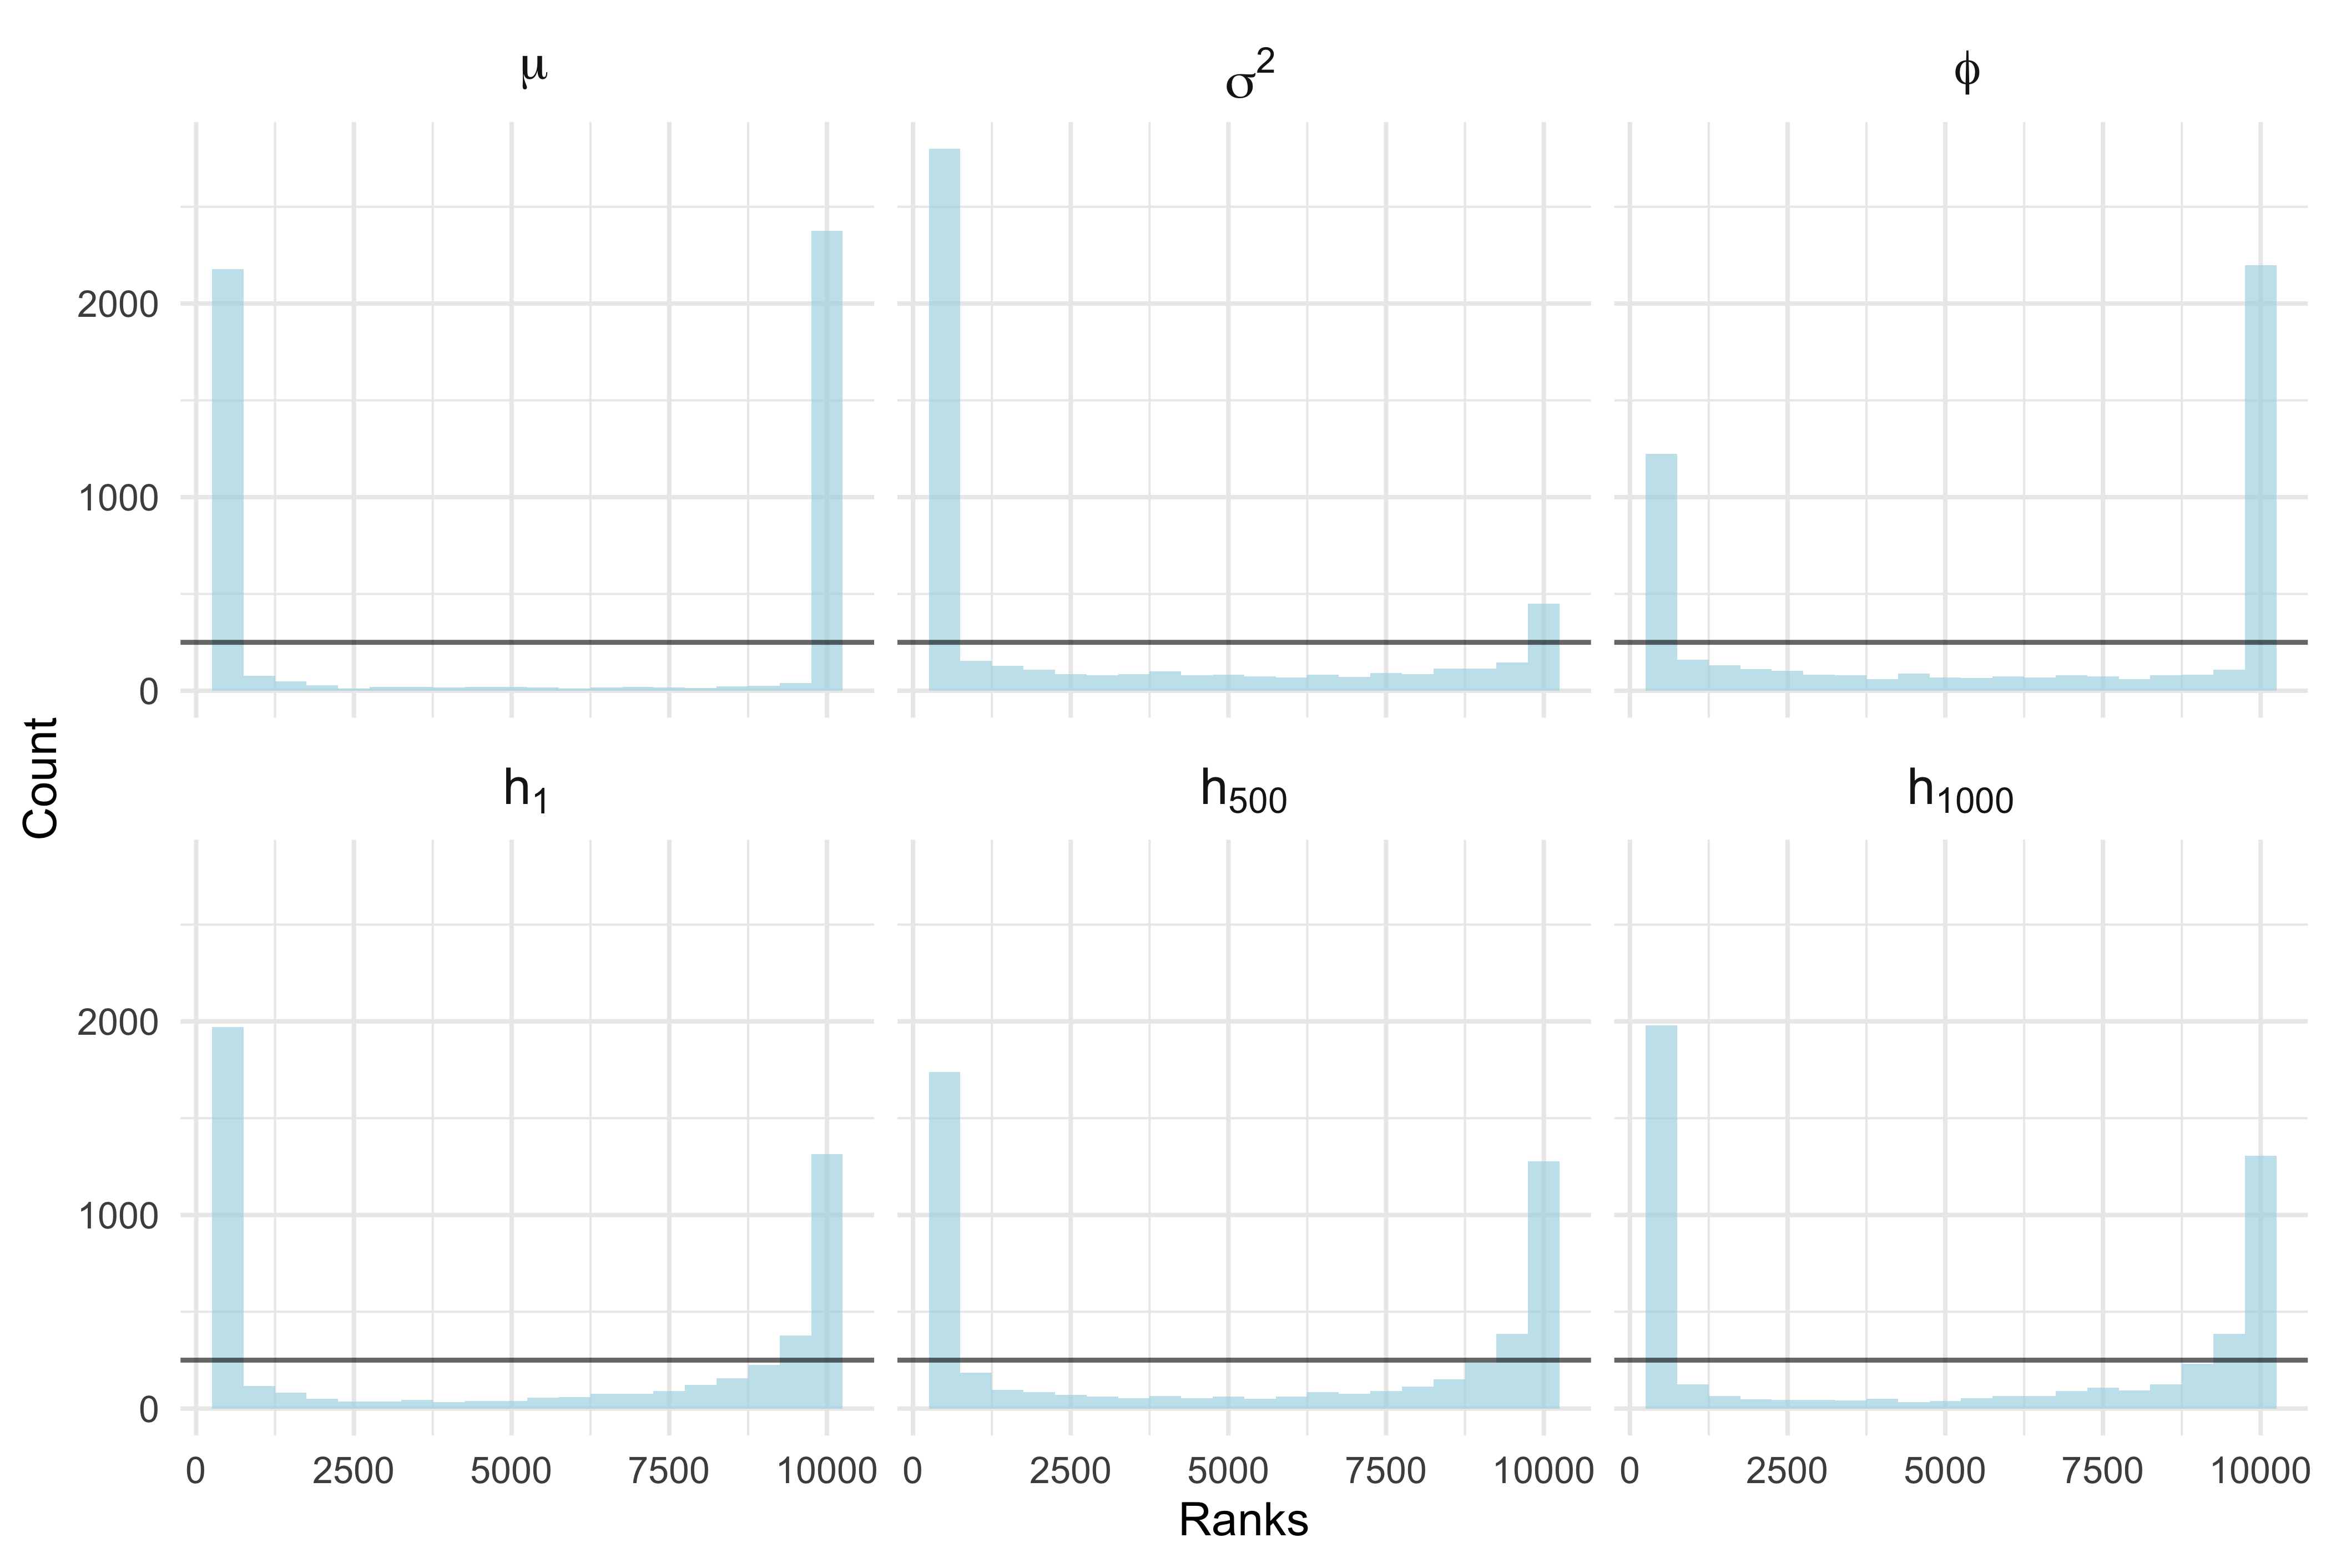
\includegraphics[scale=0.09]{results/weighted_ksc_ncp_5k.png}
    \caption{5000 SBC iterations for reweighted rank statistics from the reparameterised Gaussian mixture approximation model. No major improvements are observed to the uniformity of rank statistics.}
    \label{fig:reweight5k}
\end{figure}

\end{document}
